\chapter{The first search for \wwwlll}
\label{sec:www}
%this can have all of the details of the analysis

%1 paragraph (pg) on why this is important
%1 pg laying out the analysis design



%I'm assuming these are abbreviated here:
%MC - Monte Carlo
%LO - Leading-Order
%NLO - next-to-leading-order

%Introduction to WWW analysis
The first measurement of the $WWW$ production process
is sought by using a dataset containing 20.3 \ifb~of integrated luminosity
collected from the LHC at an energy of \energy~in 2012.
In addition to being the first study of this this particular process,
it is also the first study to search for a final state with more 
than two massive gauge bosons and one of the first studies
to be sensitive to QGCs predicted by the SM and by extension, aQGCs.
%assuming aQGCs will be defined earlier
The total \xsec for this process is expected
to be roughly $224$~femtobarns, as determined using 
\madgraph~\cite{MadGraph}. If measured, it 
would be one of the smallest \xsec measurements
within ATLAS. %with about 64\% coming from associated Higgs production.
For this search, the \www~process is studied in the 
so-called ``fully leptonic'' decay channel
where each $W$ boson decays leptonically (excluding $\tau$ lepton decays).
As can be seen in \fig\ref{fig:branching_fractions},
this decay channel occurs only about 1\% of the time,
while the rest of the time
at least one of the $W$ bosons decays hadronically.
%due to this jets problem
While the branching fraction is small,
this channel should have a smaller background than those decay 
channels that include hadronic $W$ decays.
As a result, the fully leptonic channel
is one of the most sensible channels
for obtaining sensitivity to this process.


The data is studied in a region where the signal is most prominent
with respect to the background.  This region is primarily characterized
by having three high \pt~leptons ($e$ or $\mu$), with additional
requirements determined using an optimization on the expected
measurement precision.
The signal is modeled purely using Monte Carlo (MC) simulation 
while the backgrounds are modeled using a combination of MC
simulation and data-driven techniques.
Prior to the measurement, each important background is 
studied in control regions
which are either orthogonal to the signal region selection
or where the signal is supressed.  This is to ensure that all
backgrounds are described accurately. The agreement of the data 
with the signal plus background prediction is determined using 
a ``cut-and-count'' approach where the total number of data 
events observed in the signal regions is compared to the expected number
of events from the model.
A fit to the data is performed using a profile likelihood
with the relative normalization of the signal as 
the parameter of interest and with statistical and systematic 
uncertainties treated as nuisance parameters.
%more detail? citations?
From this fit, the measured signal \xsec and uncertainty 
are extracted. The sensitivity to the signal is also evaluated
by measuring the p-value under the background only hypothesis.
In addition to measuring the SM \xsec, limits are set on 
the sensitivity to new physics in an effective field theory 
with additional aQGCs. %this aQGC stuff needs to be expanded upon greatly.



                                                                                


\begin{figure}
\centering
\includegraphics[scale=.8]{figures/branching_fractions.png}
\caption{Pie chart showing the different decay modes contributing 
to the total \xsec for the \www~process. 
The dotted areas indicate the portion of each decay 
mode which is due to the production of tau leptons.}
\label{fig:branching_fractions}
\end{figure}





\section{Data and Simulation Samples}
\subsection{Data}
\label{sec:subsection_data}


This analysis is based on the study of the full proton-proton collision
data from the LHC in 2012. The amount 
of data used in this analysis corresponds to 
an integrated luminosity of \lumi.
The uncertainty on the integrated luminosity is $1.9\%$ 
following the same methodology as in \cite{Aad:2013ucp}.
%from Van-der-Meer scans taken throughout 2012.
%read this citation.
The data are selected after requiring that at least one
of four single lepton triggers passed during data taking, 
specifically:
\begin{itemize}
\item[] Either at least one isolated electron with $\pt > 24 \GeV$
\item[] or at least one electron with $\pt > 60 \GeV$
\item[] or at least one isolated muon with $\pt > 24 \GeV$
\item[] or at least one muon with $\pt > 36 \GeV$
\end{itemize}
For the isolated lepton triggers, the isolation requirement is evaluated 
using the scalar sum of the \pt~of all tracks surrounding the lepton 
(excluding the lepton track itself) in a cone of $\Delta R < 0.2$
such the sum does not exceed 12\% (10\%) of the muon (electron)  \pt.


\subsection{Simulation samples}
%%Do I need to talk about Monte Carlo showering, 
%%hadronization and reconstruction?
%%A general discussion of Monte Carlo could go here

An important tool for the modeling of physics processes
at the LHC is Monte Carlo simulation (MC).
MC relies on random sampling to connect the matrix element formulations
derived from quantum mechanical perturbation theory into 
actual predictions for the results of proton-proton collisions
at the LHC.
The prediction of a single collision from the MC represents
one possible outcome of the proton-proton collision, with all of the 
products of the hard-scattering and their four-momenta.
This result can be passed through additional MC simulation to describe
hadronization and the soft products of the collision e.g. photon radiation.
Finally, these products are passed through a detailed 
simulation of the response of the 
ATLAS detector built in \geant~\cite{Agostinelli:2002hh}
so that the same reconstruction algorithms
can be applied as in the data.
This sampling is repeated many times to populate the 
distribution of possible
outcomes. Dedicated MC programs are provided by theorists for 
different processes to different orders in perturbation theory,
and then interfaced to different PDFs.
Details of the different processes simulated from MC and their
treatment are presented below.




\subsubsection{Signal Processes}
\label{sec:signal}


%%%
%If I'm going to include this, I better read up on it.
%%%
%The production \xsec without Higgs contribution has been calculated 
%to $\mathcal{O}(\alpha_s)$  corrections in Ref~\cite{Binoth:2008kt}.
%$\mathcal{O}(\alpha_s)$ corrections, Higgs boson exchange and spin 
%correlations of $W$ bosons lepton decay are also available
%~\cite{Campanario:2008yg}.  

The SM $WWW$ signal processes are implemented in the Monte
Carlo generator \vbfnlo~\cite{Arnold:2011wj,Arnold:2012xn},
which can generate partonic events at leading-order (LO) in QCD with
next-to-leading-order (NLO) cross-sections, 
and in \madgraph~\cite{MadGraph}, which can generate
partonic events at NLO  with NLO cross-sections. 
The partonic events are further processed 
by \pythiaeight~\cite{Sjostrand:2007gs} and \photos~\cite{Golonka:2005pn} 
to add effects of beam remnant interactions and initial and 
final state radiation. 
SM parameters must be provided to the MC generators as input. 
The most relevant input parameters are listed 
for the generators in \tab\ref{tab:signal_sm_parameters}.
The parameters are set in \pythiaeight~ using the ATLAS tune 
of AU2\cite{atlas:2011zja}.
The MC generators must also be provided an appropriate PDF.
The PDF used  in the LO \vbfnlo~generation is
the LO CTEQ6L1~\cite{Pumplin:2002vw} PDF set;
CT10 NLO~\cite{guzzi:2011sv}
is used in the NLO \vbfnlo~cross-section calculation.
The PDF used in the NLO \madgraph~generation 
and \xsec~calculation is CTEQ6L1 
but this is re-weighted to CT10 NLO using a k-factor.
Since the MC generators are computed to finite order in perturbation
theory, renormalization and factorization scales must be chosen.
The renormalization and factorization scales are dynamically
set to the $WWW$ invariant mass in the \vbfnlo~samples; they 
are set to a fixed scale equal to the $Z$ mass in \madgraph.
The \vbfnlo~samples are restricted to leptonic decays of the $W$~bosons
where each lepton has a \pt~of at least 5~\GeV. The \madgraph~
samples include all decays of the $W$~boson, with a requirement 
that jets have a a \pt~of at least 10~\GeV~ but with no requirement
on the \pt~of leptons.
The \vbfnlo~ and \madgraph~samples handle interference 
between $WH\rightarrow WWW(*)$ 
and on-shell $WWW$ production at LO, but \madgraph~is not
able to do this at NLO. As a result, the NLO \madgraph~samples
are split by on-shell \www~ and $WH\rightarrow WWW(*)$ production.
Both sets are further split by the \www~charge mode.
For each sample, the \xsecs are summarized in \tab\ref{tab:signal_xsec} 
in their full phase space and in a common fiducial phase space
defined in \sec\ref{sec:fiducial}.  
The fiducial \xsecs are observed to be nearly the same
between the two generators.
This serves as a good check of the understanding of the 
signal process. The \madgraph~\xsecs are used throughout the 
remainder of the analysis.

%Do I need to describe the k-factors?
%It would be nice to also add some distributions from Rivet comparing
%the two at truth level.


%Describe the pdf uncertainty calculation.
%what about renormalization and factorization scales




\begin{table}[ht]
\centering
\begin{tabular}{|l||c|c||}
\hline
 & \vbfnlo & \madgraph \\
\hline
\hline
Higgs mass, $m_H$ & 126.0~\GeV & \\ 
Top mass, $m_t$ & 172.4~\GeV  & \\
$Z$ mass, $m_Z$ & 91.1876~\GeV & 91.188~\GeV\\
$W$ mass, $m_W$ & 80.398~\GeV & \\
Fermi constant, $G_F$ & $1.16637\times 10^{-5}~\GeV^{-2}$ & \\
\hline
\end{tabular} 


\caption{List of the most relevant SM parameters used as input to the 
signal MC generation.}
\label{tab:signal_sm_parameters}
\end{table}


\begin{table}[ht]
\centering
\begin{tabular}{|cc||c|c|c|}
\hline
\multicolumn{2}{|c||} {Sample} &  \multicolumn{2}{c|}{Cross-section [fb]} \\
                              && Inclusive & Fiducial \\
\hline
\hline
%\multirow{3}{*}{\vbfnlo~LO} & $W^{+}W^{+}W^{-}\rightarrow l\nu l\nu l\nu$ & $3.56 \pm 0.005$ & \\
%                            & $W^{-}W^{+}W^{-}\rightarrow l\nu l\nu l\nu$ & $1.88\pm0.003$ & \\ 
%			    \cline{2-4} 
%                            & Sum & $5.44\pm0.006$ & \\ 
%\hline
\multirow{3}{*}{\vbfnlo~NLO} & $W^{+}W^{+}W^{-}\rightarrow l\nu l\nu l\nu$ & $4.95 \pm 0.007$ & $0.2050 \pm 0.0070$\\
                           & $W^{-}W^{+}W^{-}\rightarrow l\nu l\nu l\nu$ & $2.65\pm0.004$ & $0.0987 \pm 0.0037$\\ 
			    \cline{2-4} 
                           %& $WWW\rightarrow l\nu l\nu l\nu$ & $7.60\pm0.008$ & \\ 
                           & Sum & $7.60\pm0.008$ & $0.3037 \pm 0.0072$\\ 
\hline
%With PDF KFactor
\multirow{5}{*}{\madgraph~NLO} & $W^{+}W^{-}W^{+}\rightarrow \textrm{Anything}$ &$59.47\pm0.11$ & $0.0900 \pm 0.0048$\\
                        & $W^{-}W^{+}W^{-} \rightarrow \textrm{Anything}$& $28.069\pm0.076$ & $0.0476 \pm 0.0043$\\
                        & $W^{+}H\rightarrow W^{+}W^{+}W^{-}(*)\rightarrow\textrm{Anything}$ & $99.106\pm0.019$ & $0.1114 \pm 0.0029$\\
                        & $W^{-}H\rightarrow W^{-}W^{+}W^{-}(*) \rightarrow \textrm{Anything}$& $54.804\pm0.010$ & $0.0603 \pm 0.0015$\\
			\cline{2-4} 
                        & Sum & $241.47\pm0.13$ & $0.3092 \pm 0.0072$\\
%Without PDF KFactor
%\multirow{5}{*}{\madgraph~NLO} & $W^{+}W^{-}W^{+}\rightarrow \textrm{Anything}$ &$55.07\pm0.10$ & $0.0818 \pm 0.0044$\\
%                        & $W^{-}W^{+}W^{-} \rightarrow \textrm{Anything}$& $25.99\pm0.07$ & $0.0433 \pm 0.0039$\\
%                        & $W^{+}H\rightarrow W^{+}W^{+}W^{-}(*)\rightarrow\textrm{Anything}$ & $91.765\pm0.018$ & $0.1013 \pm 0.0026$\\
%                        & $W^{-}H\rightarrow W^{-}W^{+}W^{-}(*) \rightarrow \textrm{Anything}$& $50.7440\pm0.0094$ & $0.0548 \pm 0.0014$\\
%			\cline{2-4} 
%                        & Sum & $223.57\pm0.12$ & $0.2812 \pm 0.0066$\\
\hline
\end{tabular}

\caption{Inclusive and common fiducial cross-sections at NLO 
for \vbfnlo~and \madgraph~samples. 
The sum of the inclusive \xsecs are different
because of the different branching fractions in the two cases. 
The sum of the fiducial cross-sections, however, are expected to be similar because
they are computed for the same phase space, as described in \sec...}
\label{tab:signal_xsec}
\end{table}


%%%%
%soud I show the dependence on scales here?
%%%%
%The dependencies of the 
%$\xsecs on the choices of scales have been studied in the two
%references~\cite{Binoth:2008kt,Campanario:2008yg}. 

% The production at LO is a pure electroweak process. The
% NLO correction brings in $\alpha_s$ which actually makes the cross
% sections more sensitive to the choices of scales. 
%It has been pointed
%out that a jet veto should reduce the scale dependence. 

%The $W$ boson is short lived, so one must study its decay products.
%As already mentioned, the focus of this analysis is on the final state 


%need to also show the MadGraph parameters
%maybe rephrase so that I can discuss both in parallel
%get generation parameters from semi-leptonic note
%report both sets of cross-sections here
%include updated info on cross-sections and PDFs 

\begin{figure}[ht!]
\centering
\includegraphics[width=.35\columnwidth]{figures/pdf/MADppm_total_cteq6l1.png}
\includegraphics[width=.35\columnwidth]{figures/pdf/MADpmm_total_cteq6l1.png}
\includegraphics[width=.35\columnwidth]{figures/pdf/MADppm_fiducial_cteq6l1.png}
\includegraphics[width=.35\columnwidth]{figures/pdf/MADpmm_fiducial_cteq6l1.png}
\caption{The signal cross-sections for different PDFs along with their
uncertainties are shown on the {\sc MadGraph} $WWW$ signal samples
for the total $WWW$ phase space and branching fraction for
the $W^{+}W^{+}W^{-}$ (top left) and $W^{+}W^{-}W^{-}$ (top right)
charge modes
and in the fiducial region for $W^{+}W^{+}W^{-}$ (bottom left) 
and $W^{+}W^{-}W^{-}$ (bottom right).
The bands show the PDF uncertainty for CT10 NLO (solid yellow),
MSTW 2008 NLO (hashed blue), and NNPDF 3.0 NLO (hashed red). The
solid line shows the envelope of all uncertainty bands used as the final
PDF uncertainty estimate. The central value of CT10 NLO is taken as the
central value of the estimate.
The dashed-line shows the cross-section and 
statistical uncertainty for the CTEQ6L1
pdf sets used in the original generation step.}
\label{fig:signal_pdf_unc}
\end{figure}

\begin{table}[ht!]
\centering
\begin{tabular}{c|c|c}
\hline
 & \multicolumn{2}{c}{PDF Uncertainty}\\
 & $W^{+}W^{+}W^{-}$ & $W^{+}W^{-}W^{-}$ \\
\hline
\hline
Total & $+2.58\%~-2.51\%$ &  $+8.69\%~-3.47\%$ \\
Fiducial & $+3.64\%~-3.00\%$ & $+7.57\%~-3.08\%$ \\
\hline
\end{tabular}
\caption{Summary of PDF uncertainties estimated on NLO {\sc MadGraph} cross-sections
in both the fiducial and total phase space.}
\label{tab:pdfunc}
\end{table}

The uncertainty due to the choice of PDF is derived for the {\sc MadGraph} 
cross-sections following a modified version of the pdf4lhc
\cite{Botje:2011sn} recommendations.  The resulting 
uncertainty is shown separately for the two different charge modes
in both the fiducial and the inclusive phase
space in Table~\ref{tab:pdfunc}.
The uncertainty is determined by comparing three different PDFs:
CT10 NLO~\cite{Lai:2010vv}, MSTW2008 NLO~\cite{Martin:2009iq}, 
and NNPDF 3.0 NLO~\cite{Ball:2014uwa}. 
This comparison is presented in Figure~\ref{fig:signal_pdf_unc}.  
Symmetric 68\% CL uncertainties 
are determined for CT10 NLO and MSTW 2008 NLO using the 68\% CL 
set provided for MSTW directly and the 90\%CL set for CT10 after
scaling down by 
a factor of 1.645 in order to approximate a 68 \% CL uncertainty. 
The uncertainty of the NNPDF 3.0 NLO PDF set is 
determined by using the standard deviation of the distribution 
of 101 MC PDFs provided in the PDF set; the nominal value is taken
from the mean of the same PDFs.  
The CT10 NLO PDF central value is used as the nominal 
value of the final estimate.
The final PDF uncertainty on that estimate is
taken as the envelope of the uncertainty bands for all three PDF sets.  



The uncertainty on the factorization and renormalization scales are 
determined by varying each of them independently up or down by 
a factor of two. 
The effect of these variations on the cross-sections
as compared to the nominal
are shown separately for the two different charge 
modes in \tab~\ref{tab:scaleVariation}.
The symmetric uncertainty is then determined by taking the maximum 
variation for each charge mode, 
namely, 2.62\% for $W^+W^+W^-$ and 2.53\% for $W^-W^+W^-$. 

\begin{table}[ht!]
    \centering
\begin{tabular}{cc|ccc}
\hline
& \backslashbox{$\mu_F$}{$\mu_R$}     & $\frac{1}{2}M_{WWW}$ & $M_{WWW}$ &  $2M_{WWW}$ \\
\cline{2-5}
\multirow{3}{*}{\Wp\Wp\Wm} &$\frac{1}{2}M_{WWW}$ & 2.62\% & -0.14\% & -2.11\% \\
%\cline{2-5}
&$M_{WWW}$ & 2.13\% & 0 & -2.41\% \\
%\cline{2-5}
&$2M_{WWW}$ & 1.56\% & 0.24\% & -2.42\% \\
\hline
\hline
& \backslashbox{$\mu_F$}{$\mu_R$}     & $\frac{1}{2}M_{WWW}$ & $M_{WWW}$ &  $2M_{WWW}$ \\
\cline{2-5}
\multirow{3}{*}{\Wm\Wp\Wm} &$\frac{1}{2}M_{WWW}$ & 1.91\% & 1.38\% & -2.00\% \\
%\cline{2-5}
&$M_{WWW}$ & 1.61\% & 0 & -2.53\% \\
%\cline{2-5}
&$2M_{WWW}$ & 1.25\% & -1.05\% & -2.12\% \\
\hline
\end{tabular}
\caption{The relative variation of the NLO cross sections corresponding 
to different choices of factorization and renormalization 
scales for the \Wp\Wp\Wm and \Wm\Wp\Wm  processes. }
\label{tab:scaleVariation}
\end{table}

The signal cross-sections and uncertainties are thus determined to be 
\begin{equation}
\sigma^{\textrm{Total}}_{\textrm{Theory}}= 241.47\pm0.13 ~(\textrm{Stat.}) ~^{+10.33}_{-6.08} ~(\textrm{PDF}) ~\pm 6.3 ~(\textrm{Scale}) ~\textrm{fb} %uncertainty?
\end{equation}
for the inclusive \xsec and
\begin{equation}
\label{eq:fiducial_theory}
\sigma^{\textrm{Fiducial}}_{\textrm{Theory}}= 309.2\pm7.2 ~(\textrm{Stat.}) ~^{+15.05}_{-8.36} ~(\textrm{PDF}) ~\pm 8.0 ~(\textrm{Scale}) ~\textrm{ab} %uncertainty?
\end{equation}
for the fiducial cross-section.


%should i include this
%The analysis considers events with three leptons ($e$ or $\mu$) in the final state. The contributions from events in which $W$ bosons decay to $\tau$'s, and the $\tau$'s sequentially decay to $e$ or $\mu$ should be included and is expected to be 40\% of total yield of the 3-lepton final state.  


\subsubsection{aQGC signal}
blank
%
MC samples of the aQGC signal processes described in \sec\ref{sec:eft}
have been generated using \vbfnlo at NLO in QCD.  (but don't we use LO?)
The cross-sections for the aQGC signal depend on the values
of the couplings $f_{s,0}$ and $f_{s,1}$. MC samples have 
been generated for a grid of points in the $f_{s,0}$ vs $f_{s,1}$ space
and their cross-sections are shown in \fig\ref{fig:aqgc_total_xsec_ununitarized_3l}. %histogram of cross-sections

\begin{figure}[ht!]
\centering
\includegraphics[width=.8\textwidth]{figures/aQGC/total_xsec/www_3l_aqgc_total_ununitarized_noratio.png}
\caption{Total cross-section for non-unitarized aQGC signal samples as a function of $f_{s,0}$ vs $f_{s,1}$.
The total SM cross-section is shown at $f_{s,0}=f_{s,1}=0$ for comparison.}
\label{fig:aqgc_total_xsec_ununitarized_3l}
\end{figure}

The issues of unitarity violation \sec\ref{sec:eft} are taken
into account using a form factor like in \eqn\eqref{eq:form_factor}.
The choices of the exponent, $n$, and form factor scale, $\Lambda$, 
are somewhat ad-hoc. Furthermore, a complete study of the unitarity
behavior of this process has never been performed, so there are not
currently detailed prescriptions on what to choose. 
However, based on discussions with the authors of \vbfnlo, who
are at the moment trying to perform these studies, an exponent
of $n=1$ is expected to be sufficient to achieve unitarity 
for this process.  As for the choice of $\Lambda$, we have
chosen to look at a few different values, which cover a wide
range but which should follow a smooth interpolation. 
This has the advantage of providing information about the
sensitivity to the form factor that can be interpreted 
by theorists as they see fit. Dedicated MC samples
are generated with the unitarization applied for values
of $\Lambda =$ 500~\GeV, 1000~\GeV, 2000~\GeV, and 3000~\GeV.
The cross-sections for each of these unitarization cases
are shown in \fig\ref{fig:aqgc_total_xsec_unitarized_3l}.

\begin{figure}[ht!]
\centering
\includegraphics[width=.45\textwidth]{figures/aQGC/total_xsec/www_3l_aqgc_total_3TeV_noratio.png}
\includegraphics[width=.45\textwidth]{figures/aQGC/total_xsec/www_3l_aqgc_total_2TeV_noratio.png}
\includegraphics[width=.45\textwidth]{figures/aQGC/total_xsec/www_3l_aqgc_total_1TeV_noratio.png}
\includegraphics[width=.45\textwidth]{figures/aQGC/total_xsec/www_3l_aqgc_total_p5TeV_noratio.png}
\caption{Total cross-section for unitarized aQGC signal samples as a function of $f_{s,0}$ vs $f_{s,1}$.
Four different values of the unitarization scale, $\Lambda$, are chosen: 3~\TeV~(Top Left),
2~\TeV~(Top Right), 1~\TeV~(Bottom Left), and 0.5~\TeV~(Bottom Right).
The total SM cross-section is shown at $f_{s,0}=f_{s,1}=0$ for comparison.}
\label{fig:aqgc_total_xsec_unitarized_3l}
\end{figure}
























\newpage
\subsubsection{Background samples}
\label{sec:www_bg_samples}

There are other processes produced in proton-proton collisions at the LHC
which can mimic the signal processes. These are referred to as background processes.
In many cases, the background processes are either
more abundant than or of a similar abundance to
the signal. As a result, they must be well understood if there is any hope
of distinguishing between the two. The background processes to the signal
fall into two general categories: irreducible and reducible. 
The irreducible backgrounds are those that have the exact same final
state as the signal. Thus, they 
are characterized by having either exactly three prompt leptons, meaning they
come directly from the hard scattering process.
The reducible backgrounds are those which do not have the exact same
final state as the signal, but can mimic the signal in some circumstances.
For our signal, this includes backgrounds with four or more prompt leptons,
where only three leptons are measured;
two prompt leptons and an isolated photon, which can mimic an electron,
referred to as the photon backgrounds;
or two prompt leptons and a jet that mimics a lepton, referred to as
the fake backgrounds.
We treat similarly those backgrounds with three or more prompt leptons,
hereby referred to as the prompt background.
The prompt and photon backgrounds 
are estimated primarily using MC simulation while the fake background
is estimated using the data itself. 
This will be described in more detail in \sec\ref{sec:bg_fake}.
For now, we will focus only on the processes estimated using MC simulation.

Of the prompt backgrounds,
the $WZ$ process is the most important contribution since it has a 
large cross-section (compared to the signal)
and results in a final state with exactly three leptons. Another important 
prompt background is the $ZZ$ process,
which has a similar cross-section to the $WZ$ process, but is typically 
selected when 
four leptons are produced but one escapes detection.
Thus, this process is suppressed by the 
efficiency for not measuring the presence of a lepton. 
These are collectively referred to as the di-boson processes, sometimes
indicated as $VV$ where $V = W$ or $Z$\footnote{The $WW$ process is also considered
but can only produce at most two prompt leptons, making it negligible.}. 
The di-boson processes are produced using the 
\powheg~\cite{Alioli:2008gx,Nason:2004rx,Frixione:2007vw,Alioli:2010xd} generator
with the CT10 NLO PDF set and 
hadronized through \pythiaeight~using the AU2 tune, same as the signal.
Other prompt backgrounds 
include tri-boson processes like $ZWW$ and $ZZZ$ 
(referred to collectively as $VVV$)
and \ttV~production. Tri-boson processes
have cross-sections of a similar size to the signal but are suppressed 
for a similar reason
as the $ZZ$, since these can produce either four or six lepton final 
states. 
The \ttV~production process occurs when a vector
boson is produced in association with a \tt~pair. 
Since the top quark almost always decays
into a $W$-boson and a $b$-quark, \ttV~production also results in 
three vector bosons which decay into a three or four lepton
final state.
The $VVV$ and \ttV~processes were generated using \madgraph~with the 
CTEQ6L1 PDF set and hadronized
using \pythiasix~\cite{PYTHIA} with the AUET2B~\cite{atlas:2011zja} 
tune.

The photon backgrounds occur entirely from the di-boson process $Z\gamma$
where the $Z$ boson decays to two leptons and the photon mimics an electron.
A photon is measured
by observing an energy deposit in the electromagnetic calorimeter 
without any associated track in the inner detector.
A photon can mimic an electron
if it converts into an electron-positron
pair while still inside the inner detector. This leaves a track 
in the inner detector plus an energy deposit in the 
calorimeter, which is the tell-tale sign of an electron.
The $Z\gamma$ samples were generated with the \sherpa~\cite{sherpa} generator 
and the CT10 PDF set.  %hadronization? CT10 NLO? Or LO?
In addition to this process, the $W\gamma$ process behaves similarly 
but only has one prompt lepton in addition to the photon, so it is negligible.
Still, we generate it by using
the \alpgen~\cite{ALPGEN} generator with the CTEQ6L1 PDF set
and hadronize it using \jimmy~\cite{Jimmy} with the AUET2C~\cite{atlas:2011zja} 
tune.

Some of the di-boson and tri-boson processes just discussed can also be produced
through loop induced processes or double parton scattering (DPS).
The $WW$ and $ZZ$
loop induced processes are generated using the gg2ZZ~\cite{Binoth:2008pr} 
and gg2WW~\cite{Binoth:2006mf} generators with the CT10 PDF set and
hadronized using JIMMY with the AU2 tunes.
The DPS
processes are generated using \pythiaeight~with the AU2 
tunes and the CTEQ6L1 PDF set. 

The fake background is nominally estimated using the data
as described in \sec\ref{sec:bg_fake}. Some of the contributions
to this background, however, can be simulated using MC 
for cross-checks of 
the estimate from data. The main contributions
to the fake background
are the single boson processes ($V+$jets) and \tt~production.
The probability for a jet to mimic a lepton is actually quite small
and thus difficult to capture with adequate statistics using MC. 
However, these processes also have very large cross-sections.
Combining the two means that in fact the occurence of a jet mimicking
a lepton is not rare and thus non-negligible. 
The single boson $Z+$jets processes are generated using \sherpa~with the CT10
PDF set; the $W+$jets processes are generated using \alpgen~with
the CTEQ6L1 PDF set and hadronized using \jimmy~with the AUET2C tunes.
For the $Z+$jets samples, special care must be taken to remove any overlap 
between with the $Z\gamma$ simulated samples described earlier.
The \tt~processes are generated using the \mcatnlo~\cite{MCatNLO}
generator with the CT10 PDF set and hadronized in JIMMY.  %what is the tune?
Finally, the fake background also has contributions from single top production,
though it is less important. Single top production is simulated separately 
for three different production mechanisms, differing in their initial
and final states, known as
s-channel ($qb\to q't$), t-channel ($q'\overline{q}\to \overline{b}t$), 
and $Wt$-channel ($bg \to Wt$). The s-channel 
and $Wt$-channel are generated using \mcatnlo~with the CT10 PDF set and 
hadronized through \jimmy~; the t-channel is generated using 
\madgraph~with the CTEQ6L1 PDF set and hadronized 
using \pythiasix~with the AUET2B tunes.






\section{Physics Object Definition and Selection}
\label{sec:object_selection}
We attempt to identify and measure the particles coming from
the proton-proton collisions of the LHC by using the ATLAS detector.
The most interesting physics objects
for this analysis are the electrons and muons
that come from the $WWW$ decay. We also pay attention to 
the presence of hadronic activity and neutrinos, however, since these can
help discriminate the signal from the backgrounds.
Each type of particle has a unique signature in the detector
that allows us to identify the particle and reconstruct 
its properties, such as its charge and four-momentum. 
This reconstruction process does not guarantee
100\% accuracy either in identifying the particle or measuring its 
properties. As such, the reconstruction process results in reconstructed
``physics objects'' that may or may not map accurately 
to the underlying particle or physics it is trying to describe. That 
being said, this mapping is usually very successful due to the high quality
of the detector and the design of the reconstruction algorithms used.
To maximize the success of reconstruction we look at physics
objects selected only where the reconstruction is well understood.
The selections used for the physics objects of interest are described below.

%define primary vertex here
%define isolation here? or elsewhere?
%do i need to talk about object energy corrections?
%do I need to say anything about the electron tight++ or muon tight id?

Muon objects are identified by the presence of tracks in both 
the ID and the MS that are shown 
to match using an extrapolation process through the gap between the
two sub-detectors. To ensure that the track in the inner detector
indeed comes from a muon, strict requirements are placed
on the number of hits in the different sub-components of the inner detector.
%probably don't want to identify the MCP hit reqs, but I could...
The track is extrapolated back to the primary vertex and is required
to point within the boundaries of the MS and ID
within $|\eta|<2.5$.
The muon \pt~ at the primary vertex is chosen to be limited to $\pt > 10$~GeV
where there is adequate momentum resolution. We are not interested in 
muons coming from jets or other hadronic activity, therefore we
ask that they be isolated. The isolation of the muon is evaluated
in two ways: using tracks and using calorimeter deposits.
The isolation determined using tracks is calculated by adding
up the scalar sum of the \pt~ of all of the tracks (excluding
the muon track) in a cone of $\Delta R< 0.2$ from the muon track.
We ask that the isolation from tracks be less than 4\% of the muon \pt.
The isolation determined using calorimeter deposits is calculated in
a similar way except that calorimeter deposits are used instead of tracks.
We then ask that the isolation from calorimeter deposits 
be less than 7\% of the muon \pt~when $\pt < 20$~GeV and 
less than 10\% of the muon \pt~otherwise. Additional requirements
are placed upon the track extrapolation to ensure that it comes from
the primary vertex.


The signature for electron objects are that they have a track in the inner
detector that points to an energy deposit in the EM calorimeter.
The electron at the primary vertex is expected to have $\pt>10$~GeV, similar
to the muon objects. The direction of the electron energy 
deposits are also asked to fall within $|\eta| < 2.47$ and outside the 
transition region between the EM calorimeter barrel and endcap, $1.37 < |\eta| < 1.52$.
The electron objects are required to be isolated and have additional
requirements on the track extrapolation, similar to the muon objects.  
%what about further quality requirements?


Jet objects are associated with energy deposits in multiple 
neighboring cells of the EM and hadronic calorimeter systems.
Jet objects are reconstructed by grouping these cells
as topological clusters~\cite{Lampl:1099735}
using the anti-$k_t$ algorithm~\cite{Cacciari:2008gp} with $\Delta R < 0.4$.
The reconstructed jet objects are required to have 
$\pt>25$~GeV and $|\eta|<4.5$ so that
they are within the boundaries of the calorimeter systems.
The reconstructed jets are furthermore selected to suppress 
contamination from pileup events. This selection is performed by 
requiring that the majority of the
scalar sum of the \pt~of the tracks associated with the 
jet are also matched to the primary vertex. This is referred to
as the ``Jet Vertex Fraction''~\cite{Miller:1206864, ATLAS-CONF-2013-083}
and is only used for jets having $\pt < 50$~GeV and $|\eta|<2.4$, where
the algorithm is shown to perform well. Jets without any associated
tracks are always kept. 
%what about jet calibration?

It is also possible to identify jets that come from heavy flavor
decays, namely through the decays of $b$-hadron. We refer
to these as $b$-jets. A $b$-jet can frequently be identified 
because of the relatively long lifetime of the $b$ quark, which can 
result in a decay vertex that is displaced far enough
from the original primary vertex to be detected.
This can be taken advantage of to ``tag'' jets as likely coming from
$b$ quarks. A multivariate $b$-tagging algorithm~\cite{ATLAS-CONF-2014-004}
is used with a working point determined to be 85\% efficient at
identifying $b$-jets. %what about the mis-tag rate?
Often, $b$-jets are associated with physics processes other than the signal
and are helpful in identifying background processes.
As a result, we choose to veto events where 
$b$-jets are present when looking in the signal regions.


The presence of neutrinos is inferred by a momentum
imbalance in the transverse plane, referred to as the missing
transverse energy or $\MET$. The $\MET$ is calculated by 
adding up all of 
the energy deposits from calorimeters cells within $|\eta| < 4.9$
and then calibrating them based on the the reconstructed
physics object they are associated with.
If the association is ambiguous then they are chosen based on the following
preference (from most preferred to least): electrons, photons, 
hadronically decaying $\tau$-leptons, jets, and muons.
If the calorimeter deposit is not associated with any physics object
they are still considered using their own calibration.
The sum is modified to take into account the momentum of muons,
which typically leave minimum ionizing energy deposits
in the calorimeter without being completely stopped.



It is possible that the reconstructed electrons, muons, and jets
may overlap with each other inside the detector.  This can occur
because because of the same physics object being reconstructed as different
objects in the ATLAS detector.  We handle these occurrences using the following
scheme in order of precedence:
\begin{enumerate}
	\item Electron-Muon Overlap: If $|\Delta R(e,\mu)| < 0.1$, 
	then keep the muon and throw away the electron.
	\item Electron-Jet Overlap: If $|\Delta R(e,j)| < 0.2$, 
	then keep the electron and throw away the jet.
	\item Muon-Jet Overlap: If $|\Delta R(\mu,j)| < 0.2$, 
	then keep the muon and throw away the jet.
\end{enumerate}
The direction is taken from the calorimeter information for electrons,
from the combined track information for muons, and from the anti-$k_{\mathrm{T}}$
algorithm for jets.
No momentum smearing or calibration corrections
are applied to the reconstructed object directions. 
Using this scheme means that a precedence is set when 
reconstructed objects overlap such that $\mu > e > j$ where ``$>$'' should
be interpreted to mean ``is kept instead of''. 

The motivation for this scheme
is as follows. Muons will frequently radiate photons which then can pair-produce
to electrons.  If the energy of one of the pair-produced electrons is 
large enough then this can be reconstructed as well and will likely be collimated
with the muon.  Since the electron comes from the muon radiation and
since the reverse process with an electron having pair-produced muons
is heavily suppressed, the muon is kept preferentially.  The reconstruction
of overlapping electrons and jets
would rely on much of the same calorimeter energy deposits.  But the electron
reconstruction also relies on matching with a well defined inner detector
track.  It is thus assumed that if an electron overlaps with a reconstructed
jet that this is more likely to be the signature of a high energy electron.
Finally, if a muon overlaps with a jet, the muon could come from a heavy flavor 
decay. If this occurs, we choose to keep the event and consider only the muon.



\section{Event Selection}
\label{sec:event_selection}

%rewrite?
The expected number of signal events in the data is expected
to be very small compared to the background. %give a number
Fortunately, the three lepton signature of the signal allows us to
quickly throw out many events which do not look like the signal.
Still, this signature is not so unique that the background
is small enough to reveal the signal. 
Thus, we must devise a clever way to discriminate 
between the signal and these backgrounds. We select
events in two stages: first we start
by selecting events which have the general signature of the signal, 
this is referred to as the pre-selection stage; we then 
use more stringent cuts to discriminate between the signal and backgrounds, 
referred to as our signal region selection.
The signal region selection is determined by performing an 
optimization procedure starting from the pre-selection stage 
that minimizes the uncertainty
on the final measurement.  This is described in \sec\ref{sec:signal_yield}.
The signal region selection is further divided into different
categories that are each used in the final measurement
and which allows us to specially treat the different backgrounds
in each category.  
The selections used are described in more detail below.




\subsection{Pre-selection}
\label{sec:preselection}

The pre-selection is a broad selection which throws
away backgrounds that do not at all resemble the signal process.
It is mainly characterized by requiring the presence of exactly three leptons
(electron or muon) following the requirements listed in 
\sec\ref{sec:object_selection}, each with a $\pt$ of at least $20~\GeV$.
In addition, the events are required to be of good quality. This means
that the events were collected under good conditions during data taking,
both from the LHC operation and ATLAS detector operation. For instance,
during the 2012 data collection, the LAr component of the EM calorimeter
was known to occasionally produce artificial bursts of noise. These instances
were tracked and events where this occurred were thrown away. The event is 
also required to have a primary vertex with at least three associated tracks.
Finally, the event is required to pass the single lepton trigger
requirements listed in \sec\ref{sec:subsection_data} where 
at least one of the three leptons selected must have caused the trigger to fire.



\subsection{Signal Region Selection}
\label{sec:signal_regions}
The signal regions used in this analysis are separated based on the number of 
Same-Flavor Opposite-Sign (SFOS) lepton pairs selected in the event.  That is to say,
the number of lepton pair combinations in the event 
which could feasibly come from the leptonic decay of a $Z$-boson.
This results in three separate signal regions listed 
below with the lepton charge combinations
that fall in each category:
\begin{itemize}
\item \textbf{0 SFOS}: $e^{\pm}e^{\pm}\mu^{\mp}$, 
$\mu^{\pm}\mu^{\pm}e^{\mp}$ ($e^{\pm}e^{\pm}\mu^{\pm}$, 
$\mu^{\pm}\mu^{\pm}e^{\pm}$, $e^{\pm}e^{\pm}e^{\pm}$, $\mu^{\pm}\mu^{\pm}\mu^{\pm}$)
\item \textbf{1 SFOS}: $e^{\pm}e^{\mp}\mu^{\pm}$, 
$e^{\pm}e^{\mp}\mu^{\mp}$, $\mu^{\pm}\mu^{\mp}e^{\pm}$, $\mu^{\pm}\mu^{\mp}e^{\mp}$
\item \textbf{2 SFOS}: $e^{\pm}e^{\pm}e^{\mp}$, $\mu^{\pm}\mu^{\pm}\mu^{\mp}$
\end{itemize}
Note that in the 2 SFOS region, one lepton is allowed to belong to both 
pair combinations.
Those combinations listed in parentheses are not allowed for the signal based on charge conservation (neglecting charge mis-identification).  
The amount of the $W^{\pm}W^{\mp}W^{\pm}$ signal
which falls into each category is purely combinatoric.  
From the above list one can thus see that there are twice as many ways 
for the signal combinations (again neglecting those in parentheses)
to fall in the 1 SFOS regions as 
there to fall in either the 0 SFOS or 2 SFOS regions. 
Absent possible differences in signal efficiencies based on the leptons in each 
signal region, one should expect branching 
fractions of 25\%, 50\% and 25\% for the 0, 1, and 2 SFOS signal regions, respectively.


\begin{table}[ht!]
\centering
\begin{small}
\begin{tabular}{|c||c||c||c|}
\hline
&  0 SFOS  	& 1 SFOS		  & 2 SFOS  \\
\hline 
\hline 
\multirow{2}{*}{Pre-selection} & \multicolumn{3}{c|}{Exactly 3 leptons with $P_{T} > 20$~GeV}\\
                               & \multicolumn{3}{c|}{where at least one is trigger matched.  (See Section~\ref{sec:preselection}) }\\
%\hline
%Lepton $P_{T}$ 	&       \multicolumn{3}{c|}{$P_{T} > 20$~GeV}   	  \\
\hline 
b-tagged Jet Veto	& \multicolumn{3}{c|}{$N_{b-jet} = 0$ (85 \% b-tagging efficiency)} \\
\hline 
Same-Flavor Mass &	$m_{\textrm{SF}} > 20$~GeV	& \multicolumn{2}{c|}{} \\
\hline 
Z-Veto                &  $|m_{ee}-m_Z|$ & $m_{\textrm{SFOS}} < m_{Z}-35\GeV$ & $|m_{\textrm{SFOS}}-m_Z|$ \\
($m_Z = 91.1876\GeV$  &  $>15\GeV$                                         & OR   &  $>20\GeV$\\
                      & 					  & $m_{\textrm{SFOS}}>m_{Z}+20\GeV$	   &  \\
%Z-Veto                &  \multirow{3}{*}{$|m_{ee}-m_Z| > 15$~GeV} & $m_{\textrm{SFOS}} < m_{Z}-35\GeV$ & \multirow{3}{*}{$|m_{\textrm{SFOS}}-m_Z| > 20$~GeV} \\
%($m_Z = 91.1876\GeV$  &                                           & OR                                     &  \\
%                      & 					  & $m_{\textrm{SFOS}}>m_{Z}+20\GeV$	   &  \\
\hline 
Missing $E_{T}$		& 		& $E_{T}^{Miss} > 45$~GeV & $E_{T}^{Miss} > 55$~GeV \\
\hline 
Lepton-Missing $E_{T}$ Angle 	& 	\multicolumn{3}{c|}{$|\phi(3l)-\phi(E_{T}^{Miss})| > 2.5$} \\
\hline 
Inclusive Jet veto	& \multicolumn{3}{c|}{$N_{jet} \leq 1$} \\
\hline 
\end{tabular}

\end{small}
\caption{Optimized signal selection split by number of Same-Flavor 
Opposite-Sign (SFOS) lepton pairs.}
\label{tab:signal_selection}
\end{table}

Each signal region has a unique selection determined by an optmizization
procedure that minimizes the uncertainty on the expected SM measurement. 
This optimization procedure is described in detail in \sec\ref{sec:signal_yield}.
The final selection determined from the optimization
is presented in \tab\ref{tab:signal_selection}.






%other metrics like what?


%I would like to show some plots demonstrating the effect of the optimization
%One way is that I could just show all of the different points evaluated
%with their uncertainty and signal like I have shown before. 
%It might be nice to as well overlay some isoforms for different
%constant selections which could give a nice idea of the effect of diff. selections.
%But perhaps there are even better ways to visualize the effect of a 
%multi-dimensional optimization function


%It should be said that a more algorithmic way of choosing the type 
%of quantities to consider could improve this selection. Deep learning...





%this description probably belongs in an earlier section
The magnitude and direction
of the missing $E_{T}$ may be interpreted as coming from the 
vector sum of the neutrinos.  By arguments of 
symmetry, one could then compare the azimuthal direction 
of the missing $E_{T}$ to the azimuthal direction of the vector
sum of the three charged leptons. When doing so, one finds that 
in the transverse plane, 
the direction of the three charged leptons
tends to be back-to-back with the direction of the 
three neutrinos (missing $E_{T}$). The
backgrounds also show this behavior, but it is less pronounced than 
it is for the signal.  As a result, 
there is some discriminating power when cutting on the difference 
in the two angles: 
$|\Delta\phi(3l,\MET)| = |\phi(3l)-\phi(\MET)|$. 
The behavior of this quantity for signal and
background is similar in all three signal regions so based on the 
optimization it was chosen to apply the cut
$|\Delta\phi(3l,\MET)| > 2.5$ everywhere.  
We also considered taking the difference in angle between
the missing $E_{T}$ and individual leptons (e.g. the highest $\pt$ lepton) 
but this was shown to be not nearly as effective.  

Finally, the distribution of the invariant mass
from same-flavor lepton pairs (regardless of sign) 
was considered in the 0 SFOS 
region to remove any low-mass contamination from processes like from QCD.  
This was shown to offer some
modest discriminating power and a threshold of $m_{SF} > 20$~GeV 
was chosen only for the 0 SFOS region.

\subsection{Fiducial Region Selection}
\label{sec:fiducial}

A fiducial phase space or fiducial region is the 
region the analysis is sensitive to, defined 
using purely truth information (generator information before
being passed through ATLAS reconstruction).
We define our fiducial region
based on the optimized signal selection (defined at the reconstruction level)
but using only truth information. For instance, the reconstructed
lepton \pt~ requirement of 
$\pt^{\textrm{Reco}} > 20~\GeV$
is taken into account in the fiducial region selection
by requiring 
$\pt^{\textrm{Truth}} > 20~\GeV$.
By applying this for all cuts in the reconstruction selection
shown earlier in \tab\ref{tab:signal_selection},
one may compare the predicted signal yields after reconstruction
using this selection to the one in the fiducial region selection
using just truth information. Any differences are then attributed solely
to effects from reconstruction. 
The fiducial selections are determined at truth level 
using Rivet~\cite{Buckley:2010ar}, which allows for 
comparisons between different generators.


\begin{table}[ht!]
\centering
\begin{small}
\begin{tabular}{|c||c||c||c|}
\hline
&  0 SFOS  	& 1 SFOS		  & 2 SFOS  \\
\hline 
\hline 
Tau Veto & \multicolumn{3}{c|}{$N_{\tau} < 1$} \\
\hline 
Fiducial Leptons & \multicolumn{3}{c|}{Exactly 3 leptons with $p_{T} > 20~\mathrm{GeV}$ and $|\eta|<2.5$} \\
\hline 
Lepton Overlap Removal & \multicolumn{3}{c|}{$\Delta R(\ell \ell) > 0.1$}\\
\hline 
Same-Flavor Mass &	$m_{\textrm{SF}} > 20$~GeV	& \multicolumn{2}{c|}{} \\
\hline 
Z-Veto                &  $|m_{ee}-m_Z|$ & $m_{\textrm{SFOS}} < m_{Z}-35\GeV$ & $|m_{\textrm{SFOS}}-m_Z|$ \\
($m_Z = 91.1876\GeV$)  &  $>15\GeV$                                         & OR   &  $>20\GeV$\\
                      & 					  & $m_{\textrm{SFOS}}>m_{Z}+20\GeV$	   &  \\
\hline 
Missing $E_{T}$		& 		& $\MET > 45$~GeV & $\MET > 55$~GeV \\
\hline 
Lepton-Missing $E_{T}$ Angle 	& 	\multicolumn{3}{c|}{$|\phi(3l)-\phi(E_{T}^{Miss})| > 2.5$} \\
\hline 
Inclusive Jet veto	& \multicolumn{3}{c|}{$\njet \leq 1$ with fiducial jets of $p_{T} > 25~\mathrm{GeV}$ and $|\eta| < 4.5$ } \\
\hline 
\end{tabular}

\end{small}
\caption{Fiducial regions based on optimized selection.}
\label{tab:fiducial_selection}
\end{table}

The chosen fiducial region selection 
is listed in \tab\ref{tab:fiducial_selection}.
Only prompt leptons (those not originating from hadron decays) are used for 
lepton selections, and these leptons are dressed with prompt photons 
within a cone with $\Delta R = 0.1$. Generator-level jets are 
reconstructed by running the anti-kt algorithm with radius 
parameter $\Delta R = 0.4$ on all final-state particles 
after the parton showering and hadronization with the exception of prompt 
leptons, prompt photons, and neutrinos. The \MET~variable is calculated 
using all generator-level neutrinos. 
As can be seen, the selection 
in \tab\ref{tab:fiducial_selection} looks very similar to that in 
\tab\ref{tab:signal_selection} except for the object definitions
using truth information and that 
events are removed if $\tau$ leptons are present from the $W$ decays.  
Thus, the fiducial selection
does not include the branching fraction to $W\rightarrow\tau\nu$ decay, 
even though there will be some contamination from this process in the final 
reconstruction level selection. 



The fiducial cross-sections are evaluated in both 
the \vbfnlo~and \madgraph~samples mentioned in Section~\ref{sec:signal}.
The predicted fiducial cross-sections at each stage of the selection
are listed for both generators in \tab\ref{}.
The fiducial cross-sections and their
statistical uncertainties 
are summarized in each channel for both generators 
after the entire fiducial selection
in \tab\ref{tab:fiducial_cross_sections}.
They are seen to be in good agreement between both generators.


The derived fiducial cross-sections using the two generators are 
shown in Table~\ref{tab:fiducial_cross_sections}.  The cross-sections are observed
to be in good agreement between the two generators. The MadGraph NLO
fiducial cross-sections are used in the final measurement.
The PDF and scale uncertainties on the fiducial cross-sections
are determined after summing over all three signal regions 
as described earlier in \sec\ref{sec:signal}.
% it would probably be a good idea to include the fiducial cut-flows as well.





\begin{table}[ht!]
\centering
\begin{footnotesize}
\begin{tabular}{|c||c|c|}
\hline
        & \multicolumn{2}{|c|}{Fiducial Cross-section [ab]} \\
Channel & MadGraph & VBFNLO \\
\hline\hline
0 SFOS &  $114.7 \pm 4.3$     & $126.9 \pm 1.0$      \\
1 SFOS &  $126.6 \pm 4.3$     & $126.1 \pm 1.0$       \\
2 SFOS &  $50.2 \pm 2.7$     & $50.62 \pm .66$       \\
\hline
\end{tabular}

\end{footnotesize}
\caption{Fiducial cross-sections derived in each signal region for the two 
generators. Production modes are summed together to get one fiducial 
cross-section per channel per generator. The cross-sections are seen to 
be in good agreement between the two generators.}
\label{tab:fiducial_cross_sections}
\end{table}

%These have trouble with using the slashbox package
%
%include diagram

High energy electrons\footnote{Throughout this section we use 
electrons to collectively refer to both electrons and positrons
unless otherwise specified.} produced from the 
hard scatter of the proton-proton
collisions of the LHC
will frequently radiate photons in the presence of the ATLAS
detector material. Furthermore, it is also common %how common?
for high energy photons to decay into an electron-positron pair.
These two processes are shown as Feynman diagrams 
separately in \fig\ref{}.
Chaining these two processes together will cause 
an electron (positron) to radiate a photon which then produces an
electron-positron pair, resulting in a three body final state with
two electrons (positrons) and a positron (electron).
Often, the energy difference between the products in the final state will
be large, such that the most of the energy is carried away in only one
product.  It is thus possible that majority of the energy of the initial
electron (positron) is carried away in the positron (electron), which
has an opposite charge.  If the energy imbalance is large enough,
the other two final state electrons (positrons) may not have enough
energy to be reconstructed. As a result, the initial electron
(positron) will instead be measured as a positron (electron), and the 
charge of initial state electron (positron) will have effectively 
been mis-identified. 


%need to do some research on bethe-bloche.
The probability of this to occur is non-negligible in the presence of the material 
from the ATLAS detector. This is due to bremstraahlung...
Look in 'experimental foundations' and in 'particle detection'


While muons are also technically also capable of such a phenomenon, the 
energies required are too large, according to bethe-bloche.
Indeed, we observe that the rate of charge mis-identification for muons
is vanishingly small and so we neglect it. %or should I just say that it should be?

The strong dependence upon the ATLAS material means that care must be
taken when describing this process. In particular, the material 
description in MC, while sophisticated, is not perfect. Thus, the use of MC
for determining the rate of electron charge mis-identification is inherently
flawed. Instead, it would be better to use the data itself to determine
a model for these rates. 
Thus, we extract the rates of electron charge 
mis-identificatoin using the data and only use the rates determined
in MC as a cross-check.

The background due to electron charge mis-identification is most important 
for this analysis
in the 0 SFOS signal region, described in \sec\ref{sec:signal_regions},
where it is one of the only mechanisms by which the $WZ$ and $ZZ$ 
processes enter this region\footnote{The $WZ$ and $ZZ$ processes
can also enter in the 0 SFOS region if the $Z$ bosons
decay to $\tau$ leptons which then subsequently decay into 
either electrons or muons with the proper charge and flavor combination.}.
Without electron charge mis-identification, these events would fall
equally in the 1 and 2 SFOS regions.
As will be seen shortly, the overall rate of electron charge mis-identification
is quite small (calculate???). 
Furthermore, it will be seen that the total background in the 0 SFOS region is 
a good deal smaller than the the 1 and 2 SFOS regions. Thus, the
migration of events from the 1 and 2 SFOS regions to the 0 SFOS 
region, resulting from electron charge mis-identification, has
a larger relative impact on the background in the 0 SFOS 
region\footnote{There is also a migration from the 0 SFOS to the 1 and 2 SFOS 
regions, but the relative number of 0 SFOS events to 1 and 2 SFOS
events before electron mis-identification is so small as to make this
effect completely negligible.}.
As a result, we focus only on modelling the background due to electron
charge mis-identification in the 0 SFOS region and assume that an 
out of the box estimate of this background from MC is adequate for the 
1 and 2 SFOS regions.


The electron charge mis-identification background is determined
for the 0 SFOS signal region by first extracting the electron charge
mis-identification rates using the data as a model
described below. The extracted
rates are compared to an alternative method using only MC. 
The difference between the two is used as a systematic on the
rates. The rates are then used to reweight the $WZ$ and $ZZ$ MC samples
on an event-by-event basis 
according to the probability that electron charge mis-identification
could cause the event to migrate into the 0 SFOS region. In this way, 
the full statistics of the MC samples can be utilitized to get a model of
the behvaior of these processes in the 0 SFOS region, while also taking 
into account a more accurate material description. Other backgrounds
due to electron charge mis-identification are assumed to be negligible.
More details on the methods used to extract the rates and the re-weighting
method are provided below.




\subsubsection{Charge Mis-identification Rate Extraction}

The rate of electron charge mis-identification is defined as 
the probability that an electron has it's charge mis-identified.
These rates depend highly on the kinematics of the individual electrons.
In particular, the sensitivity to material dependence described above 
means that the rate depends on where in the detector the electrons
pass through. In general, the material density of the ATLAS
detector increases for high \eta~(i.e. as the electron gets closer to the
beam pipe), as seen in \sec\ref{sec:atlas_id}. The rate also increases as a function of the electron energy, 
or \pt. These are the two most important kinematic variables for determining
the rate\footnote{The material also varies as a function of the azimuthal angle,
$\phi$, in the detector. However, this is a sub-dominant effect. Furthermore,
increasing the dimensionality further significantly harms the statistical 
power of the method. Thus it is ignored.}, and 
so the rate extraction is binned as a function of both with nine $\eta$ 
bins ranging from 0 to 2.5 and six \pt~bins ranging from 15 to 120 \GeV~plus
an additional overflow bin for $\pt>120\GeV$.



The rates are studied in a region with two electrons passing the object
selection from \sec\ref{sec:www_object_selection} and that have
a di-lepton mass within 10~\GeV of the \z mass. No requirements are placed
on their charge. Two different methods
are used: one using purely MC and one using the data.
The method using MC takes $\z\rightarrow ee$ MC simulation 
and relies on being able to determine the charge of each electron from the 
\z decay by looking 
directly from at hard scattering process as provided by the generator.
This is called ``truth'' information, at which point the processes of radiation
and pair-production have not occured. It then compares
these truth electrons to the reconstructed electrons 
measured after all processes, including those of radiation and pair-production,
have been simulated and have been reconstructed
in the detector. The truth electrons and reconstructed electrons
are matched by asking that they are nearby eachother in $\eta$ and $\phi$.
The charge of the matched truth and reconstruction electrons 
are then compared and it is recorded whether or not the charges agree
in the appropriate $\pt$ and $\eta$ bin. Once all MC events
have been recorded, the rate per bin may be determined simply 
by taking the ratio of the number of electrons where the truth and reconstructed
electron charge disagreed per bin to the total number of electrons per bin. 

The nominal method for extracting the electron charge mis-identification
rates is instead one that uses the data exclusively. 
We attempt to subtract backgrounds to the $Z\rightarrow ee$
process using a method described later.
It uses the same selection as in the MC method, with the events
categorized based on whether the electrons from the \z
decay are of the same-sign or of opposite-sign.
However, in this case
there is no truth information to tell which electron's charge
has been mis-identified. Instead, we assume that those events in
the same-sign cateogry are due purely to charge mis-identification
and attempt to extract the rates by minimizing a likelihood.
Refer to the rate for an electron in a 
particular $\pt$ and $\eta$ bin $i$ as $\varepsilon_i$.
Also, refer to the total number of events observed in data with one electron
in bin $i$ and the other in bin $j$ as $N_{i,j}$.
Given the rates, the expected number of same-sign events
should be approximately $N_{i,j}(\varepsilon_i + \varepsilon_j)$,
where we have ignored the probability for both electrons to have their
charges flipped since it should be small. We do
not know the rates \emph{a priori}, but they should follow 
a Poisson likelihood given the observed total number of events,
$N_{i,j}$, and the the observed number of same sign events,
$N_{i,j}^{\textrm{SS}}$, with the following form:
\begin{equation}
\curlyl( \varepsilon_i,\varepsilon_j | N_{i,j}^{\textrm{SS}},N_{i,j})
=
\frac{(N_{i,j}(\varepsilon_i+\varepsilon_j))^{N^{\textrm{SS}}_{i,j}} e^{-N_{i,j}(\varepsilon_i+\varepsilon_j)}}{N^{\textrm{SS}}_{i,j}!}
\end{equation}
From this, we may construct a log likelihood which can be minimized
as a function of $\varepsilon_i$ and $\varepsilon_j$:
\begin{equation}
-\ln \curlyl( \varepsilon_i,\varepsilon_j | N_{i,j}^{\textrm{SS}},N_{i,j}) = 
N_{i,j}(\varepsilon_i+\varepsilon_j)
- N^{\textrm{SS}}_{i,j} \ln(N_{i,j}(\varepsilon_i+\varepsilon_j))
\end{equation}
where the terms that are not dependent on $\varepsilon_i$
and $\varepsilon_j$ have been dropped.
Thus, given the data, the values of $\varepsilon_i$ and $\varepsilon_j$
at the minimum value of the log likelihood are taken as the estimate
of the rates.

\begin{figure}[htp]
\centering
\includegraphics[width=0.45\columnwidth]{figures/ChargeMisID/Nov5_2015_TruthRates_Plot.eps}
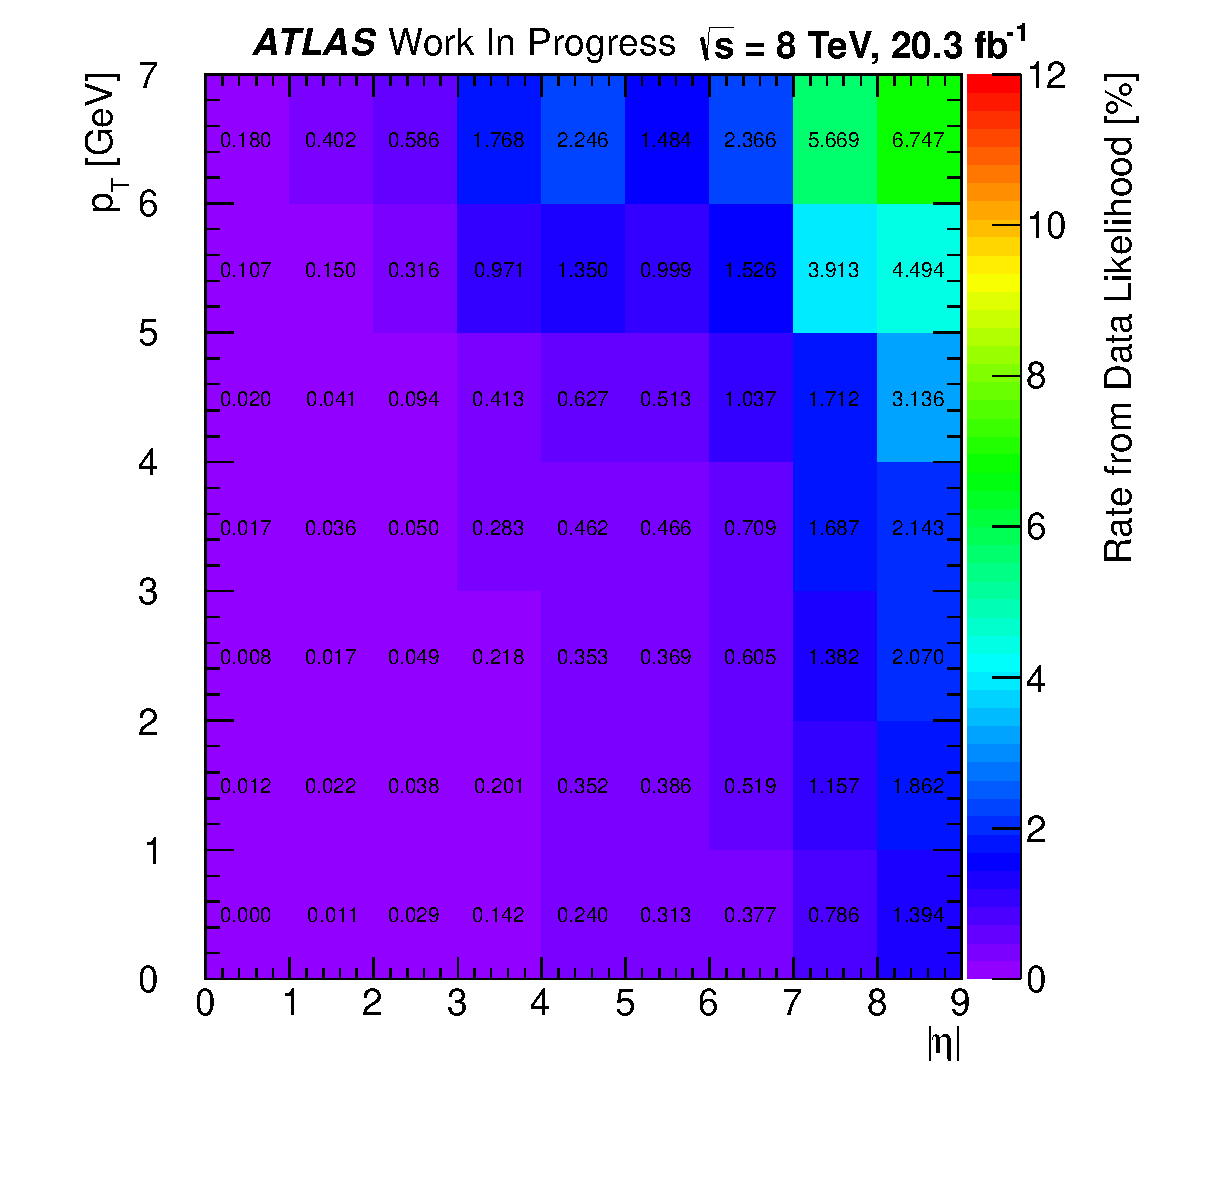
\includegraphics[width=0.45\columnwidth]{figures/ChargeMisID/Nov5_2015_DataRates_Plot.eps}
\caption{Electron charge mis-identification rates as a function of
the electron \pt and $\eta$ extracted using the MC
truth method (left) and the likelihood method in data (right). }
\label{fig:chargemisid_rates_contour}
\end{figure}

The rates for the two different methods are 
shown in \fig\ref{fig:chargemisid_rates_contour}.
For low values of \pt and $\eta$, the rate is small enough to be negligible. 
The rate increases gradually along both dimensions, reaching as much as
6.7\% in the region $\pt > 120\GeV$ and $2.4 < |\eta| < 2.5$ as measured
in the data, which corresponds to the highest bin in both dimensions. 
The rates measured using MC truth information are systematically higher
than those measured in data, almost by a factor of two. The MC simulation
tends to overestimate the amount of material (figure?) actually in the
detector, which could explain this difference....
%figure 4.45 in jinst?
%or maybe https://atlas.web.cern.ch/Atlas/GROUPS/PHYSICS/PAPERS/PERF-2013-05/
%or https://atlas.web.cern.ch/Atlas/GROUPS/PHYSICS/PAPERS/PERF-2013-03/
%might it be that the material description was improved in a later version of the MC?
%mc12b is known to have a maybe 20-30% lower rate of photon conversions overall
%according to Jake, I guess because of the material description.
%could the imporved simulation referred to in one of the papers above
%be for something that was included after mc12b? probably
%ruiqi used this sample for the MC generation:
%mc12 8TeV.147806.Powheg Pythia8 AU2CT10 Zee.merge.NTUP COMMON.e1169 s1469 s1470 r3542 r3549 p1562
%this twiki
%https://twiki.cern.ch/twiki/bin/view/Atlas/MC12cWiki?rev=3
%claims that improvements to the geometry came in mc12c
%However, these improvements claim that the improved geometry
%describes more material at high eta. It seems like this would only 
%make the disagreement between the mc and data rates, assuming
%that more material really does cause more conversion
%the paper claims the difference is in part to an incomplete
%description of SCT cooling pipes.
%the most discrepant region is between eta of 1.4 and 1.6, where the 
%difference would be consistent if material were removed.
%but this then would seem to suggest that the differences show up mostly
%in eta bin 3, which they do not. Instead it grows starting
%for eta > 2.0




%note: the material description shouldn't be affecting our zgamma
%estimate since it requires a b-layer hit so these are converting early

Some additional alternatives to these two methods are also performed
in order to better assess the performance of the mehtods
and to determine systematic uncertainties.
One alternative is to perform the same likelihood extraction
as in the data, but using only reconstructed MC. This produces
similar rates to the truth MC method, suggesting that the differences
seen between the data likelihood method and the truth MC method
are not due to the method itself. 

Another method is to extract the rates from the data with the 
likelihood method but without performing the background
subtraction mentioned earlier. In the original method, 
the background subtraction is performed by... 
...with a template fit like in \fig\ref{fig:chargemisid_fitexample}.

\begin{figure}[htp]
\centering
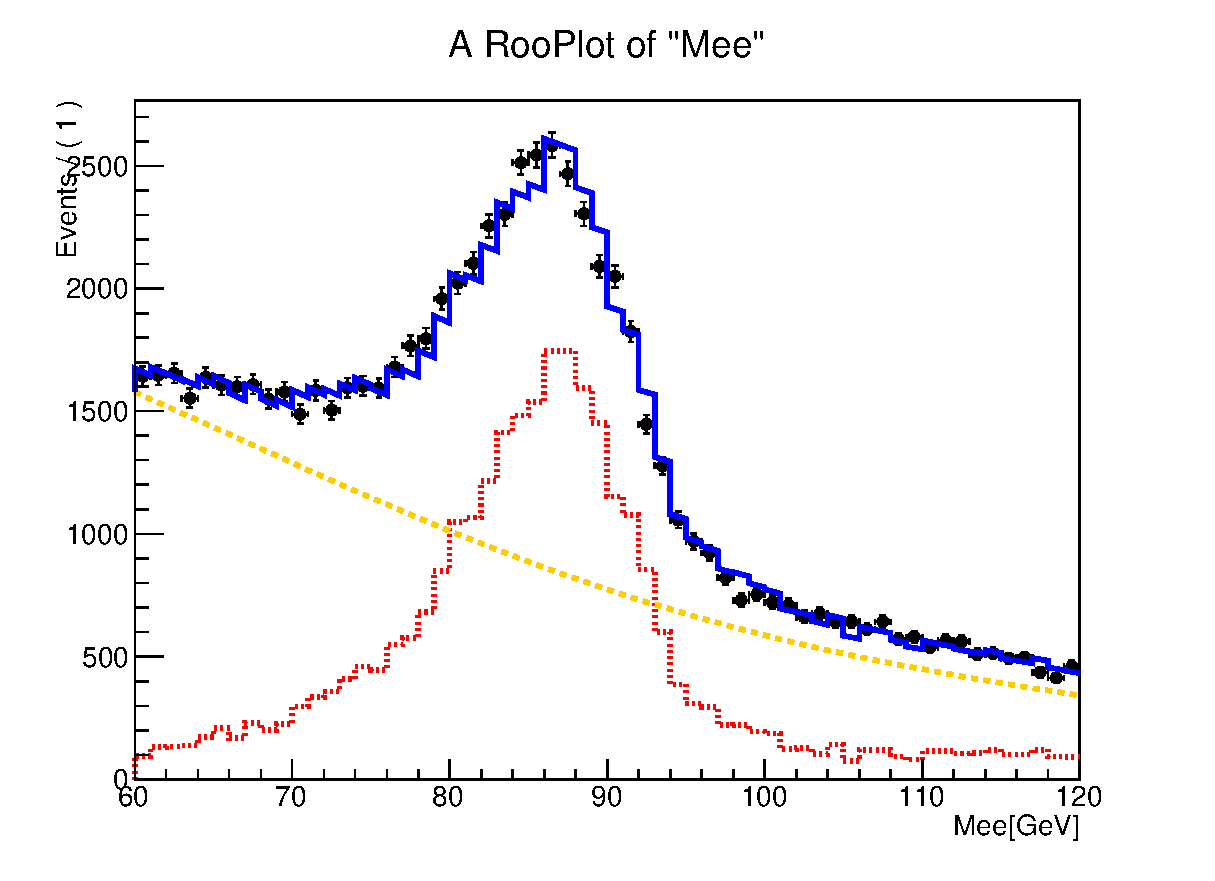
\includegraphics[width=0.6\textwidth]{figures/ChargeMisID/Tot_Polynomial_0_2.eps}
\caption{Plot of the di-lepton invariant mass 
in the region where one electron has $0 < |\eta_1| < 0.8$
and the other has $1.15 < |\eta_2|<1.6$. The data (black points)
are shown in a region where the electron isolation cuts are removed
and the electron quality requirements are loosened.
A template from $Z\rightarrow ee$ MC (red line) and a polynomial
curve (orange line) are used to fit the data. The sum of the fit
(blue line) is seen to fit the data well.}
\label{fig:chargemisid_fitexample}
\end{figure} 


The different methods of rate estimation are compared to extract
a final systematic. In \fig\ref{fig:ChargeMisID_truthRate_finalFig},
the two-dimensional rates are unfolded into one-dimension
with the bins numbered counting from low values of $\eta$ and \pt~to
high values. The nominal rate is the one shown as black points
using a likelihood fit in data with background subtraction. The vertical
bars on the black points show the statistical uncertainty on this method.
The solid black line shows the same method but without background subtraction.
These methods follow eachother quite closely, uniformly differing by 
5-6\% throughout.  The blue curve shows the rates evaluated
using the MC truth method. As was already mentioned, these tend
to be larger than the rates in data by about a factor of two. Finally, 
the red curve shows the rates evaluated using the same likelihood method
applied to the data, but using only reconstructed MC. This is seen to follow
closely the MC truth method closely, except in a few bins where the statistics
are low. The relative difference between the MC truth and MC likelihood methods
is transported to the nominal estimate in data and used as another systematic.
The difference between the methods using data and those using MC is not
used as a systematic since such a difference is expected.
The systematic uncertainties are combined in quadrature with the statistical
uncertainty on the nominal estimate to arrive at a final uncertainty on the
rates, shown as a hashed band.


\begin{figure}[htp]
\centering
\includegraphics[width=0.9\textwidth]{figures/ChargeMisID/Validation_ChargeMisIDRates_PTvsEta_FinalRateWithSys.png}
\caption{Summary of electron charge mis-identification rates using
the likelihood method in data with background subraction (black points) 
and without background subtraction (black line), the MC truth 
method (blue line), and the likelihood method in MC (red).
Systematic uncertainties are extracted as described in the text and are shown
in the gray hashed band pointing from bottom left to top right. 
The systematic uncertainties are combined with the statistical uncertainties
on the black points to arrive at a total uncertainty on the rates, shown 
in the hashed band pointing from bottom right to top left.}
\label{fig:ChargeMisID_truthRate_finalFig}
\end{figure}




\subsubsection{Di-boson MC Reweighting}


The electron charge mis-identification  rates are primarily important for the determination of the $WZ$ and $ZZ$ background contamination in the 0 SFOS region,
as mentioned already.
Once derived, the rates are applied to $WZ$ and $ZZ$ MC samples based on 
whether or not a charge flip could cause the event to appear in the 0 SFOS region.  
In particular, the following di-boson decays are considered:
\begin{itemize}
\item $WZ\rightarrow e^{\pm}\nu~ e^{+}e^{-}$
\item $WZ\rightarrow \mu^{\pm}\nu~ e^{+}e^{-}$
\item $WZ\rightarrow \tau^{\pm}\nu~ e^{+}e^{-}$
\item $ZZ\rightarrow e^{+}e^{-}~e^{+}e^{-}$
\item $ZZ\rightarrow \mu^{+}\mu^{-}~ e^{+}e^{-}$
\end{itemize}
No other decay channels are considered.  These all share in common that they 
have at least one electron-positron pair.  
Except for the $WZ\rightarrow \tau^{\pm}\nu~e^{+}e^{-}$ decay channel, 
decay channels with tau leptons are not considered
because they are suppressed by the tau branching fraction and are 
considered to be negligible.

The charge mis-identification rates are then applied to these channels on an 
event-by-event basis as follows.
For each event that is processed, its decay channel is identified 
at truth level. Each reconstructed lepton
is examined  and assigned a rate, or a probability to charge flip, 
based on its reconstructed $\pt$ and $\eta$ values.
The probability for a charge flip to occur in an event is then approximately 
the sum of rates for the individual electrons:
\begin{equation}
p(\textrm{Charge Mis-Identification in Event}) \approx \sum_{i \in \textrm{Electrons}}  \textrm{Rate}(\pt^i,\eta^i) 
\end{equation}
Higher order terms where multiple electrons are charge mis-identified is 
small and considered to be negligible.
We are only concerned with the probability that a charge flip results in the 
event falling into the 0 SFOS region. 
Consider a step function, $\Theta(e)$, defined for an individual event:
\[
\Theta(e) = 
\begin{cases}
\hfill 1 \hfill & \text{if flipping charge of $e$ classifies event as 0 SFOS} \\
\hfill 0 \hfill & \text{if flipping charge of $e$ does NOT classify event as 0 SFOS}\\
\end{cases}
\]
Then the probability that a charge mis-identification occurs and results in 
the event falling in the 0 SFOS region is:
\begin{equation}
p(\textrm{Event is classified as 0 SFOS}) \approx \sum_{i \in \textrm{Electrons}}  \textrm{Rate}(\pt^i,\eta^i)\Theta(i) 
\end{equation}
Again, we ignore the case where multiple electrons have their charge 
mis-identified.  This probability is then used as an event by event weight. 


Once the weight has been determined, we then artificially flip the charge of 
one of the electrons/positrons in the event.
If there is only one electron in the event that will lead the event 
to fall in the 0 SFOS region, its charge is flipped
and one proceeds to the next event.  However, if there are multiple electrons 
in the event, there is an ambiguity that must be resolved
about which electron's charge should be flipped. One must then be careful in 
this case to not introduce any bias.
We decided to choose a procedure where we pick a single electron from the 
event at random based on the charge flip rates
of the individual electrons. Thus, for an individual electron in an 
event, the probability that it is chosen to have its charge
flipped is:
\begin{equation}
p(\textrm{$e$ has been charge flipped}) = \textrm{Rate}(\pt^e,\eta^e)\Theta(e)~/\sum_{i \in \textrm{Electrons}} \textrm{Rate}(\pt^i,\eta^i)\Theta(i)
\end{equation}

Consider an example where the event under consideration comes from the 
decay $WZ\rightarrow e^{+}\nu e^{+}e^{-}$. Assume all three charged leptons 
pass reconstruction and are selected then label 
them as: $e^{+}_1~e^{+}_2e^{-}_3$. In this case,
the only way that this event could be classified as 0 SFOS when 
flipping the charge of only one electron/positron is to flip the 
charge of the electron.
Thus, $\Theta(e^{+}_1)=\Theta(e^{+}_2)=0$ and $\Theta(e^{-}_3)=1$.  The event 
weight will then be equal to the rate of charge mis-identification 
for  $e^{-}_3$ and it will have it's charge flipped to be positive.

Now consider an example of an event with 
the decay of $ZZ\rightarrow \mu^{+}\mu^{-}~ e^{+}e^{-}$.
If all four leptons are reconstructed and selected, the event will not 
be considered at all in the three lepton selection of this analysis, so 
consider the case where the $\mu^{+}$ is not selected leaving three leptons 
labeled as: $\mu^{-}_1 e^{+}_2 e^{-}_3$.  The probability for the muon to 
charge flip is negligible which leaves the electron and the positron. Flipping 
the charge of either one at a time will result in the event being 
classified as 0 SFOS.  Thus, in
this case $\Theta(\mu^{-}_1)=0$ and $\Theta(e^{+}_2)=\Theta(e^{-}_3)=1$. The 
event weight will then be the sum of the rates for $e^{+}_2$ and $e^{-}_3$.
The probability that the electron has its charge flipped is then 
$\frac{\textrm{Rate}(e^{-}_3) }{ \textrm{Rate}(e^{+}_2)+ \textrm{Rate}(e^{-}_3)}$ 
and similarly for the positron.

\subsubsection{Validation}
This procedure has been validated on the $WZ$ and $ZZ$ samples by comparing 
the predictions taken directly from MC to the predictions reweighted in the 
0 SFOS signal region using the procedure just described. This is done in 
Figure~\ref{fig:ChargeMisID_Validation_WZ} for the $WZ$ samples and on 
Figure~\ref{fig:ChargeMisID_Validation_ZZ} for the $ZZ$ samples. It can be seen 
the agreement in the shape looks good for all the distributions. An offset 
between the two distributions is observed. This difference is covered partially by 
the systematic uncertainties of the method.  Any remaining difference could 
be expected from the difference in rates observed at high $\eta$ and 
high $E_{T}$ as seen in Fig.~\ref{fig:ChargeMisID_truthRate_finalFig} and 
serves as justification for using the data-driven method.

There is no special treamtent of the charge mis-identification contribution to 
other background contributions in the 0 SFOS region or to any contributions to the 
1 and 2 SFOS signal regions, including diboson processes, as the effect is 
expected to be very small.  Any charge mis-identification events are thus 
taken directly from MC in this case.


 \begin{figure}[htp]
 \centering
 \includegraphics[width=0.4\textwidth]{figures/ChargeMisID/Validation_ChargeMisIDRates_WZ_PTLepton.png}
 \includegraphics[width=0.4\textwidth]{figures/ChargeMisID/Validation_ChargeMisIDRates_WZ_EtaLepton.png}
 \includegraphics[width=0.4\textwidth]{figures/ChargeMisID/Validation_ChargeMisIDRates_WZ_DeltaPhi.png}
 \includegraphics[width=0.4\textwidth]{figures/ChargeMisID/Validation_ChargeMisIDRates_WZ_MET.png}
 \includegraphics[width=0.4\textwidth]{figures/ChargeMisID/Validation_ChargeMisIDRates_WZ_Mee.png}
 \includegraphics[width=0.4\textwidth]{figures/ChargeMisID/Validation_ChargeMisIDRates_WZ_JetMultiplicity.png}

 \caption{Validation of the charge mis-ID rates comparing 
 MC $WZ\rightarrow \ell ee$ ($\ell=e,\mu$) samples reweighted with the 
 charge misID rates measured in the MC $Z\to{}ee$ 
 sample to the original MC predictions. Distribution of 
 lepton $p_{T}$, $\eta$, $\Delta \phi(3l,E_{T}^{Miss})$,\met{}, Same-sign 
 di-electron invariant mass, and jet multiplicity.}
 \label{fig:ChargeMisID_Validation_WZ}
 \end{figure}
 
 
 \begin{figure}[htp]
 \centering
 \includegraphics[width=0.4\textwidth]{figures/ChargeMisID/Validation_ChargeMisIDRates_ZZ_PTLepton.png}
 \includegraphics[width=0.4\textwidth]{figures/ChargeMisID/Validation_ChargeMisIDRates_ZZ_EtaLepton.png}
 \includegraphics[width=0.4\textwidth]{figures/ChargeMisID/Validation_ChargeMisIDRates_ZZ_DeltaPhi.png}
 \includegraphics[width=0.4\textwidth]{figures/ChargeMisID/Validation_ChargeMisIDRates_ZZ_MET.png}
 \includegraphics[width=0.4\textwidth]{figures/ChargeMisID/Validation_ChargeMisIDRates_ZZ_Mee.png}
 \includegraphics[width=0.4\textwidth]{figures/ChargeMisID/Validation_ChargeMisIDRates_ZZ_JetMultiplicity.png}

 \caption{Validation of the charge mis-ID rates comparing 
 MC $ZZ\rightarrow \ell \ell ee$ ($\ell=e,\mu$) samples reweighted with the 
 charge misID rates measured in the MC $Z\to{}ee$ 
 sample to the original MC predictions. Distribution of 
 lepton $p_{T}$, $\eta$, $\Delta \phi(3l,E_{T}^{Miss})$,\met{}, Same-sign 
 di-electron invariant mass, and jet multiplicity.}
 \label{fig:ChargeMisID_Validation_ZZ}
 \end{figure}



  
%\input{www_estimate_charge_misid}
\subsection{Fake lepton background}
\label{sec:bg_fake}

This background consists of the events with at least one non-prompt lepton denoting the hadrons misidentified as leptons and leptons originating from heavy-flavour decays, such as $b-$meson decays. We refer to these non-prompt leptons as ``fake'' leptons and subsequently refer to prompt leptons as ``real'' leptons. It is estimated using a generalised matrix method \cite{Arguin:1558979,Gillam:2014xua} which is a fully data-driven technique. All leptons are firstly classified as ``loose'' or ``tight'' according to their identification and/or isolation quality. The loose leptons must pass all lepton preselection requirements and fail any of the signal selection criteria defined in Tables \ref{tab:eledef} and \ref{tab:muondef}. Once the efficiencies for real and fake preselected leptons to satisfy the tight lepton selections are measured, the number of events with fake lepton background can be predicted. This measurement is done as a function of $\pt$. %and/or \pt\ bin.


\tabcolsep=0.11cm
\begin{table}[ph!]
\begin{center}
\small{
    \begin{tabular}{lc}
%      \hline
%      Cut            & Value/description \\
      \hline
      \hline
      \multicolumn{2}{c}{\textbf{Preselected electron}}\\
      \hline
      Algorithm      & Central Electrons (author is 1 or 3)\\
      \hline
      Acceptance     & $\pt > 10\,\GeV, |\eta| < 2.47$ excluding crack region \\
      \hline
      Quality & \texttt{Medium++} \\
%      \hline
%      Further cuts & not touching dead OTX region\\
      \hline
      Impact parameter & $|d_0/\sigma(d_0)| < 3.0$\\ 
      & $|z_0 \cdot sin(\theta)|<$ 0.5 mm \\
      \hline
      $e$-$e$ isolation             & $\Delta{}R(e,e)>0.2$ \\
      \hline
      $e$-$\mu$ isolation      & $\Delta{}R(e,\mu)>0.2$ \\
      \hline
      \multicolumn{2}{c}{\textbf{Signal electron}}\\
      \hline
      Quality & \texttt{Tight++} \\
%      \hline
%      Track   & with match \\
      \hline
      Track isolation   & \pt cone20/\pt $<0.04$\\
      \hline
      Calorimeter isolation & \ET cone20/\ET$<0.10$\\% for \pt$>20$\GeV\\
      					  % & \ET cone20/\ET$<0.07$ for \pt$<20$\GeV\\
     \hline
     \hline
\end{tabular}
}
\end{center}
\caption{Summary of the electron selection criteria used for the global matrix method. The signal requirements defined in Section~\ref{sec:Object_selection} are applied on top of the lepton preselection.}
\label{tab:eledef}
\end{table}

\tabcolsep=0.11cm
\begin{table}[ph!]
  \begin{center}%\renewcommand\arraystretch{1.2}
  \small{
    \begin{tabular}{lc}
%      \hline
 %     Cut            & Value/description \\
      \hline
      \hline
      \multicolumn{2}{c}{\textbf{Preselected muon}}\\
      \hline
      Algorithm      & STACO combined \\
      \hline
      Acceptance     & $\pt > 10\,\GeV, |\eta| < 2.5$ \\
      \hline
      Quality        & Tight    \\
      \hline
      Inner detector track quality & MCP ID Hits selection\\
      \hline
            Impact parameter & $|d_0/\sigma(d_0)| < 3.0$\\ 
      & $|z_0 \cdot sin(\theta)|<$ 0.5 mm \\
      \hline
      $\mu$-$\mu$ isolation             & $\Delta{}R(\mu,\mu)>0.2$ \\
      \hline
      \multicolumn{2}{c}{\textbf{Signal muon}}\\
      \hline
      Track isolation   & \pt cone20/\pt $<3.0$\\
      \hline
      Calorimeter isolation & \ET cone20/\ET $<0.10$\\% for \pt$>20$\GeV\\
      						%& \ET cone20/\ET $<0.07$ for \pt$<20$\GeV\\
      \hline
      \hline
    \end{tabular}
    }
  \end{center}
   \caption{Summary of the muon selection criteria used for the global matrix method. The signal requirements defined in Section~\ref{sec:Object_selection} are applied on top of the lepton preselection.} 
    \label{tab:muondef}
\end{table}

\subsubsection{Generalized matrix element method}

The advantage of the matrix method used in this analysis is that an arbitrary number of preselected leptons can be present in the event. In case of single lepton events, the equation relating the number of events with real ($n_R$) and fake ($n_F$) lepton in $\pt$ bin $i$ to the expected number of events with the lepton reconstructed as tight ($n_T$) or loose ($n_L$) can be written as following:
\begin{align*}
  \begin{pmatrix} n_T \\ n_L \end{pmatrix} 
  &= 
  \begin{pmatrix}
  \varepsilon_i & \zeta_i \\ 1-\varepsilon_i & 1-\zeta_i
  \end{pmatrix} 
  \begin{pmatrix} n_R \\ n_F \end{pmatrix}
\end{align*}
where $\varepsilon_i$ and $\zeta_i$ are the real and fake efficiencies measured in $\pt$ bin $i$. Given the measurements of $n_T$ and $n_L$, the expected real and fake contributions can be calculated from the inverted relation:
\begin{align*}
  \begin{pmatrix} n_R \\ n_F \end{pmatrix} 
  &= 
  \frac{1}{\varepsilon_i-\zeta_i}
  \begin{pmatrix}
  1-\zeta_i & -\zeta_i \\ \varepsilon_i-1 & \varepsilon_i	
  \end{pmatrix} 
  \begin{pmatrix} n_T \\ n_L \end{pmatrix}
\end{align*}
%Take an event selection requiring exactly one baseline lepton, which we additionally require to pass tight quality requirements. We have measured nT and nL, and want n'T the expected number of tight leptons that are fake.
%The procedure to obtain an estimate for the fake lepton contribution passing the tight requirements $n'_T$ in single lepton events is:
The procedure to obtain an estimate for the number of fake leptons passing the tight requirements $n'_T$ is:
\begin{align*}
  \begin{pmatrix} n'_T \\ n'_L \end{pmatrix} 
  &= 
  \begin{pmatrix}
  \varepsilon_i & \zeta_i \\ 1-\varepsilon_i & 1-\zeta_i
  \end{pmatrix} 
  \begin{pmatrix} 0 \\ n_F \end{pmatrix}
  =  
  \begin{pmatrix}
  \varepsilon_i & \zeta_i \\ 1-\varepsilon_i & 1-\zeta_i
  \end{pmatrix} 
  \begin{pmatrix}0&0\\0&1\end{pmatrix} 
  \begin{pmatrix} n_R \\ n_F \end{pmatrix}\\
  &=
  \begin{pmatrix}
  \varepsilon_i & \zeta_i \\ 1-\varepsilon_i & 1-\zeta_i
  \end{pmatrix} 
  \begin{pmatrix}0&0\\0&1\end{pmatrix} 
  \frac{1}{\varepsilon_i-\zeta_i}
  \begin{pmatrix}
  1-\zeta_i & -\zeta_i \\ \varepsilon_i-1 & \varepsilon_i	
  \end{pmatrix} 
  \begin{pmatrix} n_T \\ n_L \end{pmatrix}
\end{align*}
This is typically calculated as a weight $w_i$ for each event where the lepton in \pt\ bin $i$ is either tight ($n_T=1$ and $n_L=0$) or loose ($n_T=0$ and $n_L=1$).

For compactness, it is useful to introduce the following notation where summation convention is implied over repeated indices:
\begin{align*}
  r = \begin{pmatrix} n_R \\ n_F \end{pmatrix} , \quad
  t = \begin{pmatrix} n_T \\ n_L \end{pmatrix} , \quad
  \phi  = 
  \begin{pmatrix}
    \varepsilon_i & \zeta_i \\
    1-\varepsilon_i & 1-\zeta_i
  \end{pmatrix} 
  \quad\Rightarrow
  \quad
  t_\beta = {\phi}_\beta^{\ \alpha} r_\alpha
\end{align*}
where $\alpha$ takes values corresponding to $R$ or $F$, and similarly $\beta$ for $T$ or $L$. The expected number of tight leptons that are fake is then:
\begin{align*}
  t'_\nu = {\phi}_\nu^{\ \mu} \omega_\mu^{\ \beta} {{\phi}^{-1}}_\beta^{\ \alpha} t_\alpha
\end{align*}
where $\omega$ represents the selection of only the expected fake component. 

In case of an event with $N$ preselected leptons, the formula can be written in this compacted notation as following:
\begin{align*}
  t'_{\nu_1\cdots\nu_N} = \phi_{\nu_1}^{\ \mu_1}\cdots\phi_{\nu_N}^{\ \mu_N}\ \omega_{\mu_1\cdots\mu_N}^{\ \beta_1\cdots\beta_N}\ {\phi^{-1}}_{\beta_1}^{\ \alpha_1}\cdots{\phi^{-1}}_{\beta_N}^{\ \alpha_N} t_{\alpha_1\cdots\alpha_N}.
\end{align*}
Each $\phi$ is computed with the efficiencies $\varepsilon$ and $\zeta$ appropriate for the lepton index. The ``real/fake configuration selector'' $\omega$ picks out the sets of indices ${\beta_i}$ corresponding to components one wish to count as fake background. In general, it looks like:
\begin{align*}
  \omega_{\mu_1\cdots\mu_N}^{\ \beta_1\cdots\beta_N} = \delta_{\mu_1}^{\ \beta_1}\cdots\delta_{\mu_N}^{\ \beta_N} \ f(\beta_1,\,\ldots,\,\beta_N)
  % \omega_{\mu_1\cdots\mu_N}^{\ \beta_1\cdots\beta_N} = \delta_{\mu_1}^{\ \beta_1}\cdots\delta_{\mu_N}^{\ \beta_N} \ f(\beta_1,\,\ldots,\,\beta_N,\nu_1,\,\ldots,\,\nu_N)
\end{align*}
where $\delta_i^j$ is the Kronecker delta and $f$ is a function of the indices taking values 1 (for a fake combination) and 0 (for a real combination).
%where the function $f$ takes values 0 or 1 to pick out the sets of indices ${\beta_i}$ that correspond to components we wish to count as fake background. In general it will depend on the output tight/loose configuration being computed, and we choose it such that the number of real leptons (out of the $N$ in the event) in the intermediate configuration $\{\beta\}$ is less than the number of tight leptons in the output configuration $\{\nu\}$.

This method assigns a set of weights for each event with $N$ leptons and a measured tight/loose combination -- one for each output tight/loose configuration separately. Therefore, for each of these matrix method output combinations, different leptons will be defining the event and passing through the signal selections. It is important to stress that the correlations between each configuration must be taken into account.
%
%For each event with $N$ leptons and a measured tight/loose combination $\{\alpha\}$, this method hence gives a weight for each output tight/loose combination $\{\nu\}$. Since, for each of these combinations, different leptons will be defining the event, each combination is propagated through the final channel selection and trigger matching procedure separately, with the leptons being treated as tight or loose according to the output of the matrix method. Variables such as invariant mass of $Z$ boson are also computed using the appropriate leptons.
%
%For example, if one measures an event with three pre-selected leptons,
%$e^+e^-\mu^+$, with configuration TLL, then the matrix method will produce
%the following
%\begin{align*}
%  \textrm{\textbf{Input}} \qquad\qquad & \qquad\qquad\textrm{\textbf{Output}} \\
%  e^+e^-\mu^+, TLL \longrightarrow& \left\{
%  \begin{array}{ll}
%    LLL & w_{LLL} \quad e^+_Le^-_L\mu^+_L \quad \textrm{Fails cuts} \\
%    \cdots & \cdots \\
%    TTL & w_{TTL} \quad e^+_Te^-_T\mu^+_L \quad \textrm{Fails cuts} \\
%    TLT & w_{TLT} \quad e^+_Te^-_L\mu^+_T \quad \textrm{Fails cuts} \\
%    LTT & w_{LTT} \quad e^+_Le^-_T\mu^+_T \quad \textrm{Fails cuts} \\
%    TTT & w_{TTT} \quad e^+_Te^-_T\mu^+_T \quad \textrm{Exactly 3 leptons with 1SFOS}
%  \end{array}
%  \right.
%\end{align*}
%Of the possible combinations, only one passes the signal selection cuts,
%presuming trigger matching, $b$-jet veto and other requirements are also satisfied.

For example, if one measures an event with four preselected leptons,
$e^+e^-e^+\mu^+$, with configuration TTLL, then the matrix method will produce
the following:
\begin{align*}
  \textrm{\textbf{Input}} \qquad\qquad & \qquad\qquad\textrm{\textbf{Output}} \\
  e^+e^-e^+\mu^+, TTLL \longrightarrow& \left\{
  \begin{array}{ll}
    LLLL & w_{LLLL} \quad e^+_Le^-_Le^+_L\mu^+_L \quad \textrm{Fails cuts} \\
    \cdots & \cdots \\
    TTTL & w_{TTTL} \quad e^+_Te^-_Te^+_T\mu^+_L \quad \textrm{Exactly 3 leptons with 2SFOS} \\
    TTLT & w_{TTLT} \quad e^+_Te^-_Te^+_L\mu^+_T \quad \textrm{Exactly 3 leptons with 1SFOS} \\
    TLTT & w_{TLTT} \quad e^+_Te^-_Le^+_T\mu^+_T \quad \textrm{Exactly 3 leptons with 0SFOS} \\
    LTTT & w_{LTTT} \quad e^+_Le^-_Te^+_T\mu^+_T \quad \textrm{Exactly 3 leptons with 1SFOS} \\
    TTTT & w_{TTTT} \quad e^+_Te^-_Te^+_T\mu^+_T \quad \textrm{Fails cuts}
  \end{array}
  \right.
\end{align*}
If one presumes that trigger matching and other requirements are satisfied, only four of all possible combinations pass the event pre-selection cuts. In addition, each of these ``subevents'' falls into specific channel according to the number of same flavour opposite sign (SFOS) pairs.

To propagate uncertainties on the efficiencies, the derivatives of $t'_{\nu_1\cdots\nu_N}$ with respect to $\varepsilon_i$ and $\zeta_i$ for each lepton $i$ need to be calculated. This can be evaluated exactly and efficiently at runtime. Correlations between the real efficiencies $\varepsilon$ measured in different  $\pt$ bins are neglected since the uncertainty on the measurement is small. Correlations between the fake efficiencies $\zeta$ binned in \pt\ are preserved by propagating the systematic variation for each bin separately. Finally, there is a statistical correlation between two output configurations from one input event falling into one signal region which need to be taken into account. Using the previous example, the variance of each subevent in 1SFOS treated as separately is $w^2_{TTLT}$ and $w^2_{LTTT}$. However, it should be in fact $(w_{TTLT} +w_{TTLT})^2$. %for a signal region 1SFOS

\subsubsection{Real lepton efficiency}

The efficiencies for real preselected leptons to pass the tight requirements are measured in data as a function of the lepton $\pt$. The measurement is performed in data samples enriched with real leptons from $Z\rightarrow l^+l^-$ decay with a standard tag-and-probe method. The tag passes all signal lepton selections and is trigger matched, while the requirement imposed to the probe is to satisfy only the lepton preselection cuts. Their invariant mass has to be within $Z$-mass window: $m_{ll}\in[80, 100]$~\GeV{}. If both leptons satisfy the tag requirements, they are alternatively considered as the tag in order to avoid any bias introduced by its selection. The invariant mass for two opposite sign same-flavour leptons is illustrated in Fig. \ref{fig:realEff_CRs}.

The $\pt$ distributions for both the number of probes passing the signal requirements, $n^{\mathrm{Tight}}$, and the total number of probes, $n$, are shown separately in the electron and muon control regions used to derive the rates in Figure~\ref{fig:realEff_CRsPt}.
The efficiency, $\varepsilon_i$, is calculated in each $\pt$ bin, $i$, by taking the ratio of $n_{i}^{\mathrm{Tight}}$ over $n_i$. That is,
\begin{align*}
%\varepsilon_i=\frac{n_T^{\mathrm{probe}}}{n^{\mathrm{probe}}}
\varepsilon_i=\frac{n_{i}^{\mathrm{Tight}}}{n_{i}}
\end{align*}
The final binning of the efficiency is chosen to be coarse enough
to have good statistics in the ratio while also preserving shape information as a function
of $\pt$. 
The final efficiencies determined using both data and MC 
can be seen in Fig. \ref{fig:realEff}.

Two sources of systematic uncertainties are taken into account. Firstly, the measurement may be affected by the selection of $20$~\GeV\ $Z$-mass window. It has been thus varied by $5$~\GeV\ and the final effect has been proved to be negligible. Secondly, the measurement is done in Drell-Yan data without any  specific treatment of the other background. Therefore, the difference between the efficiencies measured in data and MC is taken as a systematic.  A summary of the rates measured in
data and MC used to compute the systematic uncertainties are shown for electrons
in Table~\ref{table:realEff_El} and for Muons in Table~\ref{table:realEff_Mu}.

\begin{figure}[h!]
\centering
\subfigure{
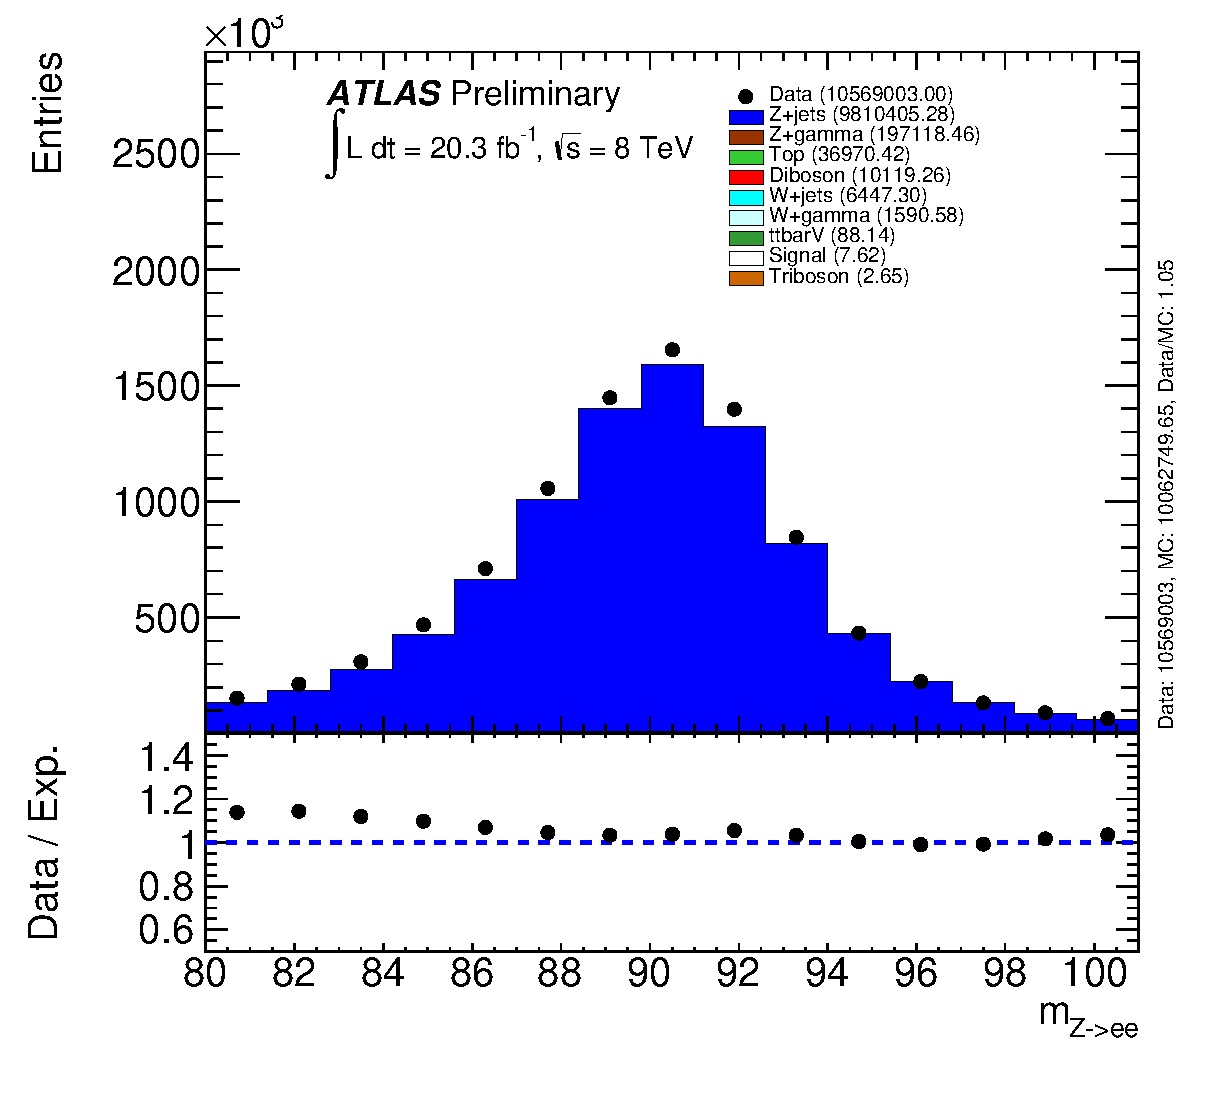
\includegraphics[width=0.4\columnwidth]{figures/fakes_bkg/CRs/hPtElectronZBosonloosecut_total_new.eps}
}
\centering
\subfigure{
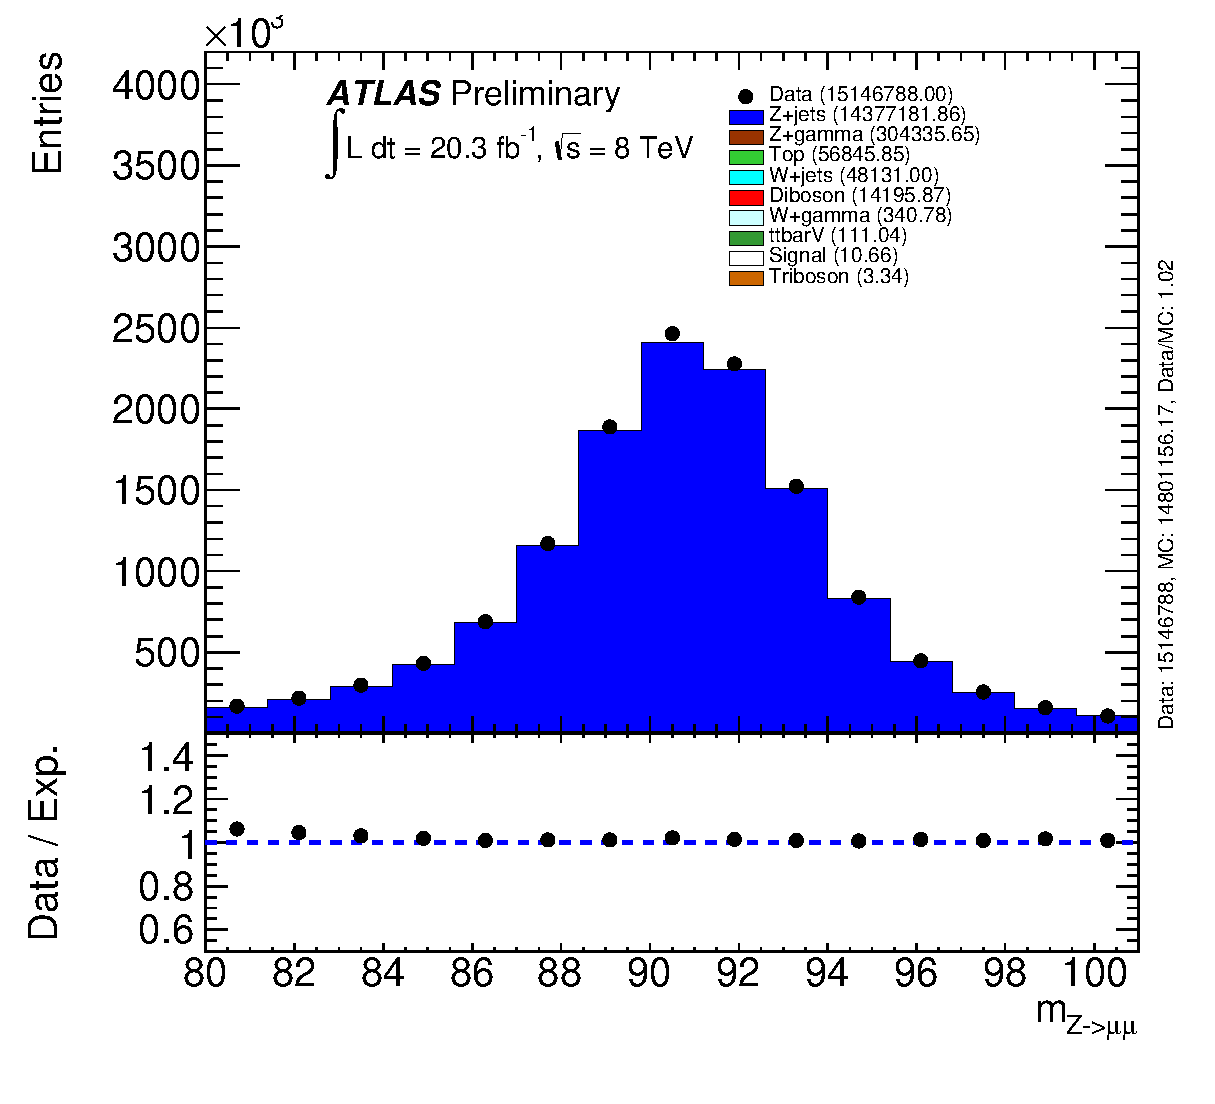
\includegraphics[width=0.4\columnwidth]{figures/fakes_bkg/CRs/hPtMuonZBosonloosecut_total_new.eps}
}
\vspace{-10mm}\caption{Invariant mass distribution of two opposite charge and same flavor di-lepton invariant mass electrons (left) and muons (right).}
\label{fig:realEff_CRs}
\end{figure}


\begin{figure}[h!]
\centering
\includegraphics[width=0.4\columnwidth]{figures/fakes_bkg/CRs/RealTP/ProbeTightElectronPt_histratio.png}
\includegraphics[width=0.4\columnwidth]{figures/fakes_bkg/CRs/RealTP/ProbeTightMuonPt_histratio.png}
\includegraphics[width=0.4\columnwidth]{figures/fakes_bkg/CRs/RealTP/ProbeElectronPt_histratio.png}
\includegraphics[width=0.4\columnwidth]{figures/fakes_bkg/CRs/RealTP/ProbeMuonPt_histratio.png}
\caption{Probe lepton \pt\ distributions in SFOS tag and probe control regions used to derive real rates.  Electron (left) and muon (right) are shown
when the probe lepton is either tight (top) or no additional selection (besides the preselection) is required (bottom)}
\label{fig:realEff_CRsPt}
\end{figure}


\begin{figure}[h!]
\centering
\includegraphics[width=0.45\columnwidth]{figures/fakes_bkg/Efficiencies/ElectronRealRates.png}
\includegraphics[width=0.45\columnwidth]{figures/fakes_bkg/Efficiencies/MuonRealRates.png}
\caption{Real lepton efficiency as a fucntion of \pt\ and measured in data (red) and MC (blue) for electrons (left) and muons (right).}
\label{fig:realEff}
\end{figure}

\clearpage

%\tabcolsep=0.11cm
\begin{table}[h!]
\centering
\begin{tabular}{|l||c|c||c|c||c|}
\hline
&\multicolumn{2}{c||}{Data}&\multicolumn{2}{c||}{MC}&\multicolumn{1}{c|}{}\\ & $\varepsilon_r$ & $\sigma_{stat}$ & $\varepsilon_r$ & $\sigma_{stat}$ & $\sigma_{sys}$\\ 
\hline\hline
%$p_{T}\in[10,15]$ GeV &  $0.6285$ &  $0.0034$ &  $0.6420$ &  $0.0036$ &  $0.0135$\\ 
%$p_{T}\in[15,20]$ GeV &  $0.6960$ &  $0.0024$ &  $0.7056$ &  $0.0025$ &  $0.0096$\\ 
$p_{T}\in[20,30]$ GeV &  $0.8105$ &  $0.0011$ &  $0.8134$ &  $0.0013$ &  $0.0028$\\ 
$p_{T}\in[30,50]$ GeV &  $0.8732$ &  $0.0005$ &  $0.8794$ &  $0.0006$ &  $0.0062$\\ 
$p_{T} > 50$ GeV &  $0.9097$ &  $0.0012$ &  $0.9150$ &  $0.0012$ &  $0.0053$\\ 
\hline
\end{tabular}

\caption{Measured real efficiencies for electrons including statistical and systematic absolute uncertainties. 
Systematic is calculated by taking the difference
between the efficiencies measured in data and MC.  The efficiency measured in data is used as the nominal central value.
} 
\label{table:realEff_El}
\end{table} 

%\tabcolsep=0.11cm
\begin{table}[h!]
\centering
\begin{tabular}{|l||c|c||c|c||c|}
\hline
&\multicolumn{2}{c||}{Data}&\multicolumn{2}{c||}{MC}&\multicolumn{1}{c|}{}\\ & $\varepsilon_r$ & $\sigma_{stat}$ & $\varepsilon_r$ & $\sigma_{stat}$ & $\sigma_{sys}$\\ 
\hline\hline
%$p_{T}\in[10,15]$ GeV &  $0.8684$ &  $0.0033$ &  $0.8763$ &  $0.0036$ &  $0.0079$\\ 
%$p_{T}\in[15,20]$ GeV &  $0.8906$ &  $0.0024$ &  $0.8956$ &  $0.0025$ &  $0.0050$\\ 
$p_{T}\in[20,30]$ GeV &  $0.9217$ &  $0.0010$ &  $0.9291$ &  $0.0012$ &  $0.0074$\\ 
$p_{T}\in[30,50]$ GeV &  $0.9700$ &  $0.0004$ &  $0.9737$ &  $0.0006$ &  $0.0038$\\ 
$p_{T} > 50$ GeV &  $0.9862$ &  $0.0011$ &  $0.9878$ &  $0.0011$ &  $0.0017$\\ 
\hline
\end{tabular}

\caption{Measured real efficiencies for muons including statistical and systematic absolute uncertainties.
Systematic is calculated by taking the difference
between the efficiencies measured in data and MC.  The efficiency measured in data is used as the nominal central value.
} 
\label{table:realEff_Mu}
\end{table} 


\clearpage

\subsubsection{Fake lepton efficiency}

The fake efficiency represents the probability that a fake lepton satisfying the preselected criteria passes also the signal requirements. 
The measurement, performed separately for each $\pt$ bin, $i$, is performed in fake-enriched samples by looking at the number of probe leptons in data 
passing preselection, $n_i$, and comparing to the number which only pass also the tight
selection, $n^{Tight}_i$. Contamination from real leptons, $n^{\mathrm{Real}}_i$ and $n^{\mathrm{Tight}, \mathrm{Real}}_i$, 
and from photon converted leptons, $n^{\mathrm{PC}}_i$ and $n^{\mathrm{Tight},\mathrm{PC}}_i$, 
is corrected using MC by subtracting from the totals.  The rate is then determined as follows:
%\begin{align*}
\begin{equation}
\zeta_i=\frac{n^{\mathrm{Tight}}_i-n^{\mathrm{Tight},\mathrm{Real}}_i-n^{\mathrm{Tight},\mathrm{PC}}_i} {n_i -n^{\mathrm{Real}}_i -n^{\mathrm{PC}}_i }
\label{eq:fakerate}
\end{equation}
%\end{align*}
Since the rates depend on the fake lepton origin, the derivation is done separately for electrons and muons.     

The classification of leptons in MC as being either real or from photon conversion is performed on an event-by-event basis at truth level using the MCTruthClassifier tool~\cite{MCtruthclassifier:twiki}.  
Since this is a dilepton control region, the majority of events with a real lepton
tag and a probe lepton due to photon conversion comes from the $W\gamma$ process where the photon converted lepton is an electron.
As expected, the number of probe muons coming from photon conversion are observed to be negligible.

Efficiencies are measured from a data set enriched with one tight lepton that passes the signal lepton selections with \pt$>40$~\GeV\ and 
one fake candidate satisfying only the preselection criteria defined in tables~\ref{tab:eledef} and~\ref{tab:muondef}. Events with additional loose or tight leptons are rejected. 
The QCD background may also enter these control regions, especially in low \met\ . Therefore, an additional \met$>10$~\GeV\ requirement is introduced. 
In order to reduce the contamination from real processes like $t\bar{t}$, $WW$ and $Z$, the two leptons are required to have the same sign.
Finally, the control regions are split based on the flavor of the tag and probe leptons.  The muon rates are determined in the region
with two muons while the electron rates are determined in the region with a muon tag and an electron probe.  The choice of a muon tag 
in the region used to derive the electron rates is particularly important since allowing electron tags have a large contamination from $Z$ backgrounds.
This is true even after the same-sign requirement because of charge mis-identification.  
The charge mis-identification rate for muons is negligible
and so allows one to use the muon-muon control region for the muon rates, which has the least contamination.
This behavior can be seen in the distributions of probe muon transverse momentum in the same-sign muon-muon tag-and-probe control region used to derive
the muon fake rates shown in Fig.~\ref{fig:fakeEff_CRs_muon} while
the distributions of probe electron transverse momentum are shown in the same-sign electron-muon tag-and-probe control region used to derive
the electron fake rates shown in Fig.~\ref{fig:fakeEff_CRs_electron}.
The control regions for both electrons and muons are further split based on the number of b-tagged jets in the event, 
which has an effect on the source of the fake leptons.  In particular, requiring b-tagged jets increases the fraction
of fake leptons coming from heavy flavor. Two different sets of control regions were ultimately considered, those
with at least one b-tagged jet and those without any requirement on the presence of b-tagged jets.  The region
with at least one b-tagged jet ($N_{b-jet} > 0$) is used as the central value since it contains more heavy flavor contributions
and so compares better with the signal regions, as described later in Section~\ref{sec:fakecomposition}.  The other is used 
to determine a systematic on the composition, described later.  


A detailed breakdown of the numbers used to compute the fake rates are shown in Appendix~\ref{sec:appendix_fakebg}.
%would it be useful to show the other dilepton control regions in an appendix?

Three systematic uncertainties are considered. First, the subtraction of the processes with 
two real leptons ($t\bar{t}V$, $VV$ and $VVV$) using MC prediction introduced an uncertainty on 
their cross-sections. This effect is estimated by varying the MC normalization by $\pm 20$\%.  %should rerun with 5%
We refer to this is as the 'correlated' systematic uncertainty.
Second, given that the extraction regions and the signal regions have different kinematic selections, 
the fake leptons of different origin dominate. This kinematic dependence of fake efficiencies has been estimated 
by modifying the requirements of the sample used for the measurement. In particular, the cut thresholds 
on the $E_{T}^{Miss}$ and tag lepton $\pt$ used
for determining the dilepton control regions are varied. The $E_{T}^{Miss}$ threshold is 
varied in 5~GeV steps scanning a range of $\pm 10$~GeV around the nominal
threshold of $E_{T}^{Miss} > 10$~GeV while the $\pt$ threshold is varied in 5~GeV steps in a range of $\pm 20$~GeV 
around the nominal threshold of $\pt > 40$~GeV.  When varying the $E_{T}^{Miss}$ cut, the $\pt$ cut
is kept at the nominal threshold and vise-versa. This is referred to as the 'uncorrelated' systematic.
These are determined separtely for electrons and muons, since they use different control regions. The 'uncorrelated' and
'correlated' systematics for electrons and muons are then combined together by adding in quadrature on an event-by-event basis.
As a result the uncertainty is presented as a single systematic uncertainty on the fake electron
contribution and a separte single systematic on the fake muon contribution.
The third and final systematic contribution comes from the choice of control region, based on the number of b-tagged
jets, as described earlier.  The nominal control regions for both the electron and muon cases is when 
there is at least one b-tagged jet present.  The difference between the rates for the nominal case
and the region where no requirement is placed on the presence of b-tagged jets is chosen as a systematic.
We have determined that the difference in the composition in these two regions adequately covers the difference
in composition that may be present due to the extrapolation from the control regions to the signal regions. This is 
discussed in more detail in Section~\ref{sec:fakecomposition}.  Another set of control regions was studied
which vetos any b-tagged jets, but this was observed to give a very large difference in composition which is 
probably too conservative of an estimate to be used as a reasonable systematic.
The rates along with the statistical and systematic uncertainties are summarized in Fig.~\ref{fig:fakeEff} 
as well as in Tables \ref{table:fakeEff_El} and \ref{table:fakeEff_Mu}.
The final binning of the efficiency is chosen to be coarse enough
to have good statistics in the ratio while also preserving shape information as a function
of $\pt$. 


%\begin{figure}[h!]
%\centering
%\subfigure{
%\includegraphics[width=0.3\columnwidth]{figures/fakes_bkg/CRs/CR1N_probePt_all_total.eps}
%}
%\centering
%\subfigure{
%\includegraphics[width=0.3\columnwidth]{figures/fakes_bkg/CRs/CR2N_probePt_all_total.eps}
%}\\ 
%\vspace{-14mm}
%\subfigure{
%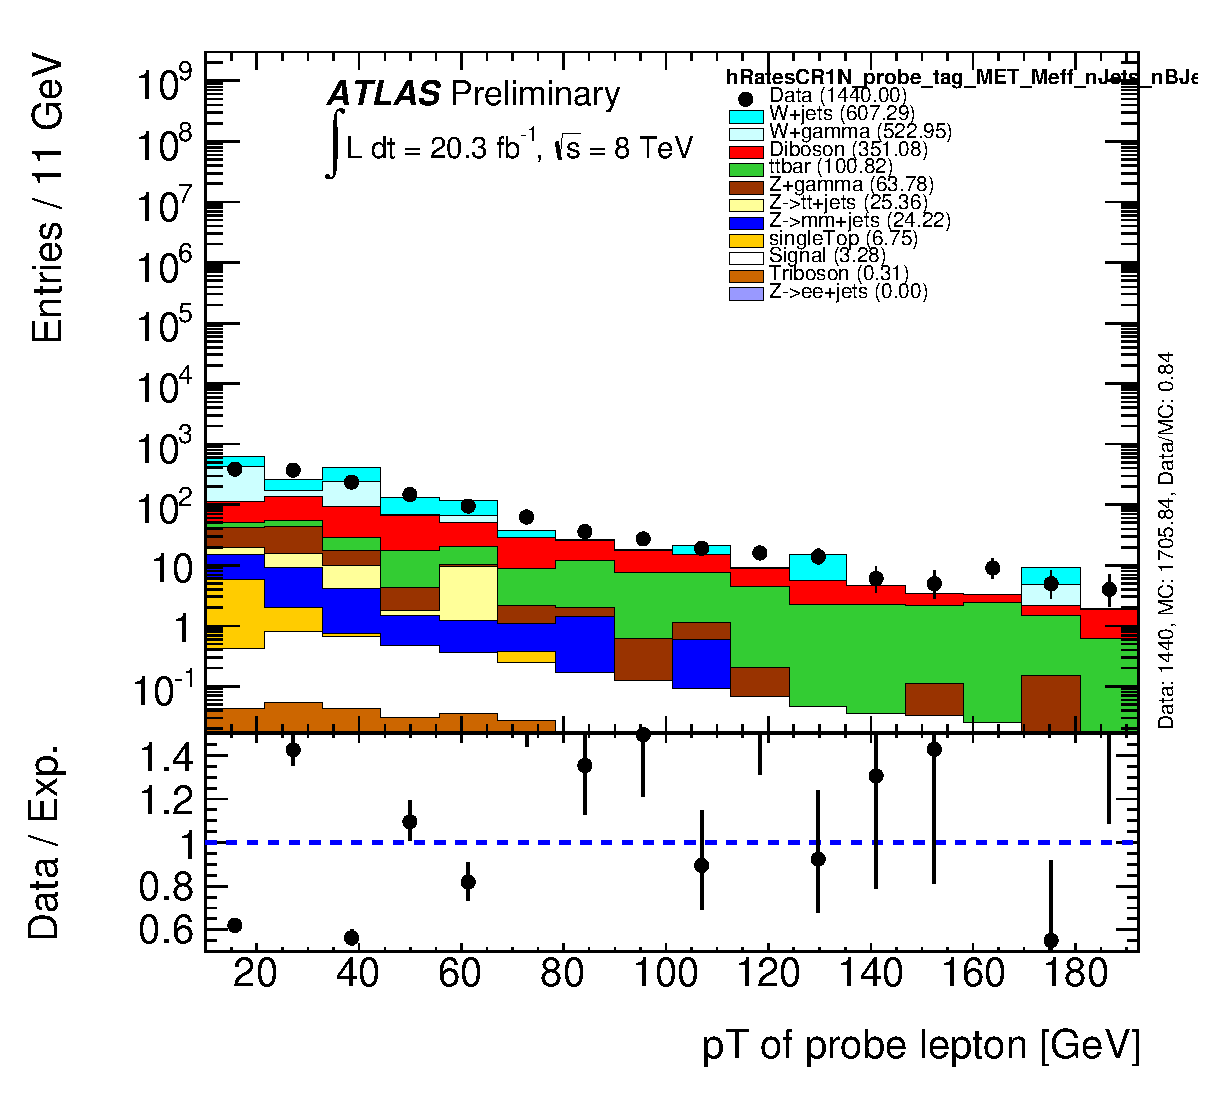
\includegraphics[width=0.3\columnwidth]{figures/fakes_bkg/CRs/CR1N_probePt_tight_total.eps}
%}
%\centering
%\subfigure{
%\includegraphics[width=0.3\columnwidth]{figures/fakes_bkg/CRs/CR2N_probePt_tight_total.eps}
%}
%\vspace{-10mm}\caption{Transverse momentum distributions \pt\ of probe electron (left) and muon (right) in the control regions. The probe passes pre-selection (top) and signal (bottom) criteria.}
%\label{fig:fakeEff_CRs}
%\end{figure}


\begin{figure}[h!]
\centering
\subfigure{
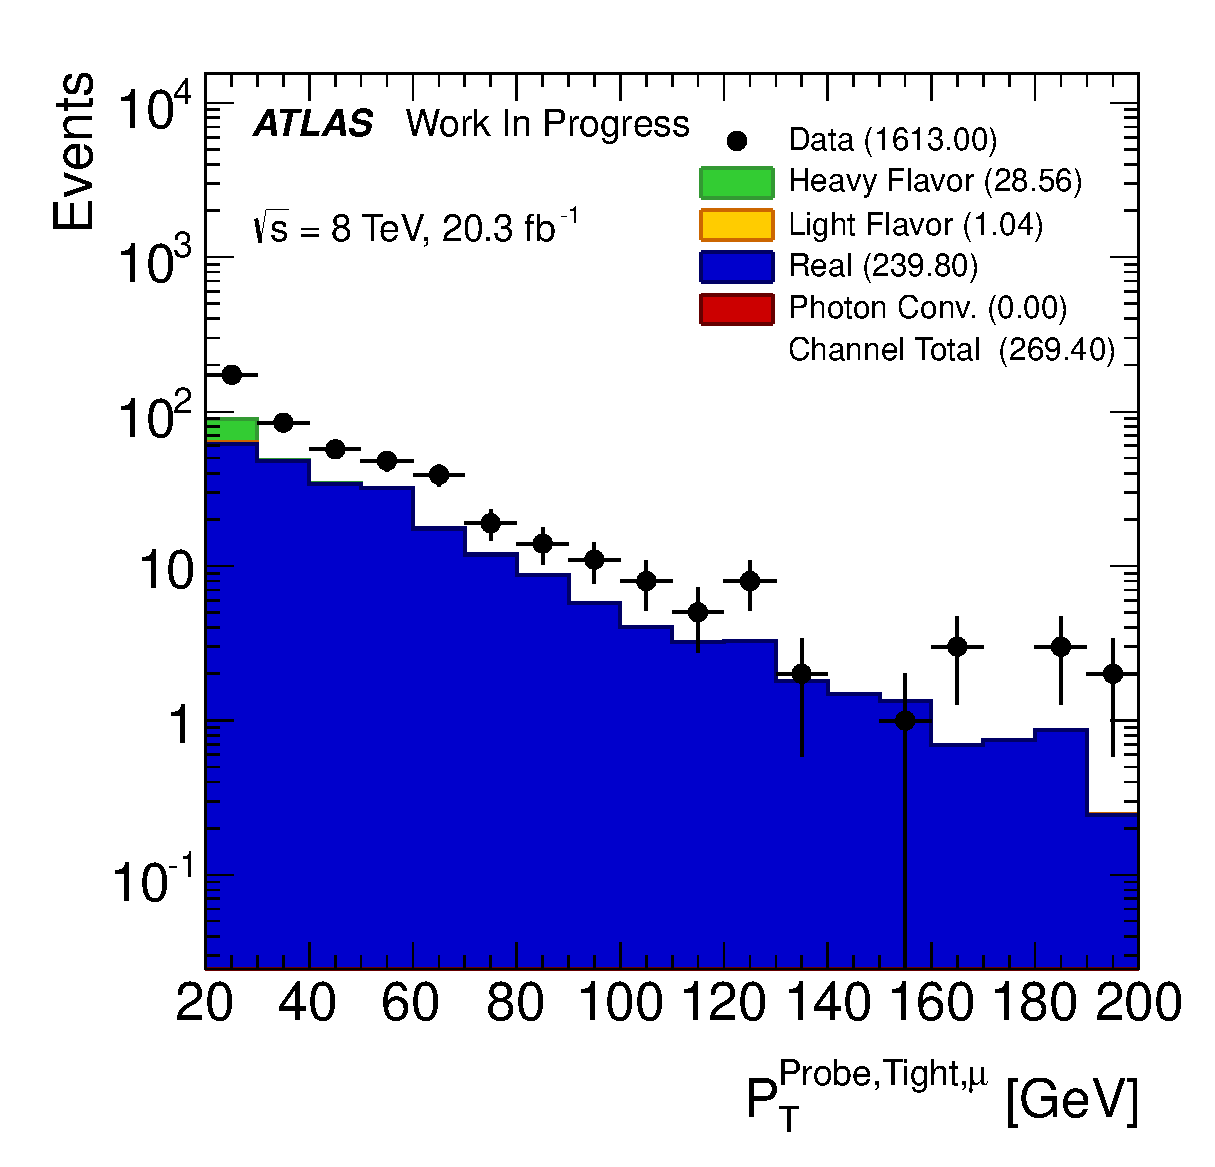
\includegraphics[width=0.45\columnwidth]{figures/fakes_bkg/CRs/SameSignMuonMuon/NoStack/ProbeTightMuonPt.eps}
}
%\centering
%\subfigure{
%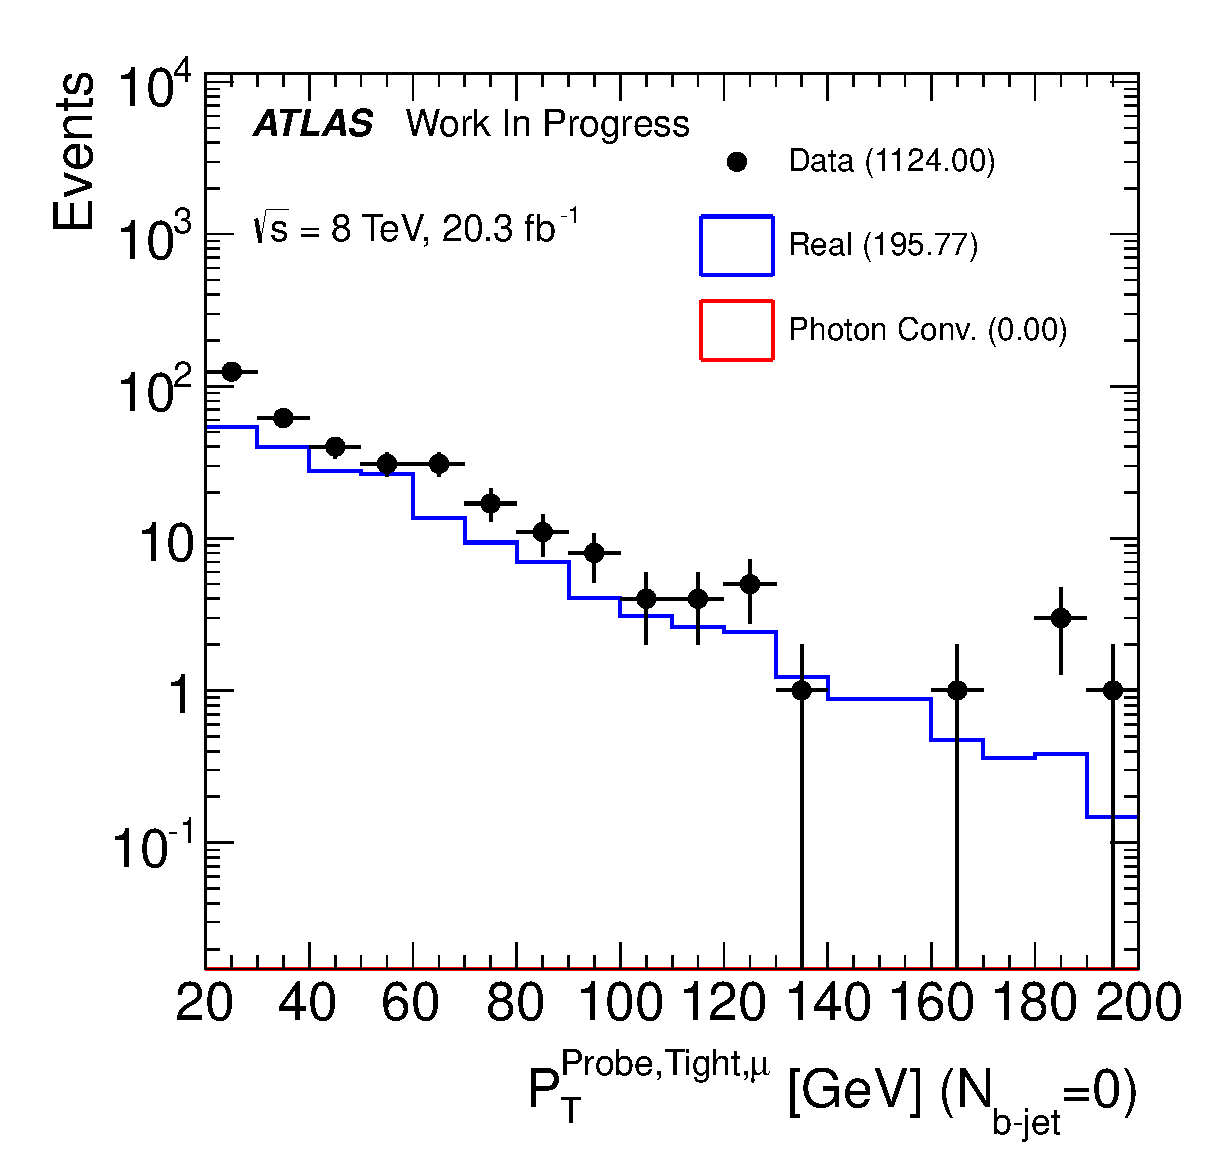
\includegraphics[width=0.3\columnwidth]{figures/fakes_bkg/CRs/SameSignMuonMuon/NoStack/ProbeTightMuonPtBJetEq0.eps}
%}
\centering
\subfigure{
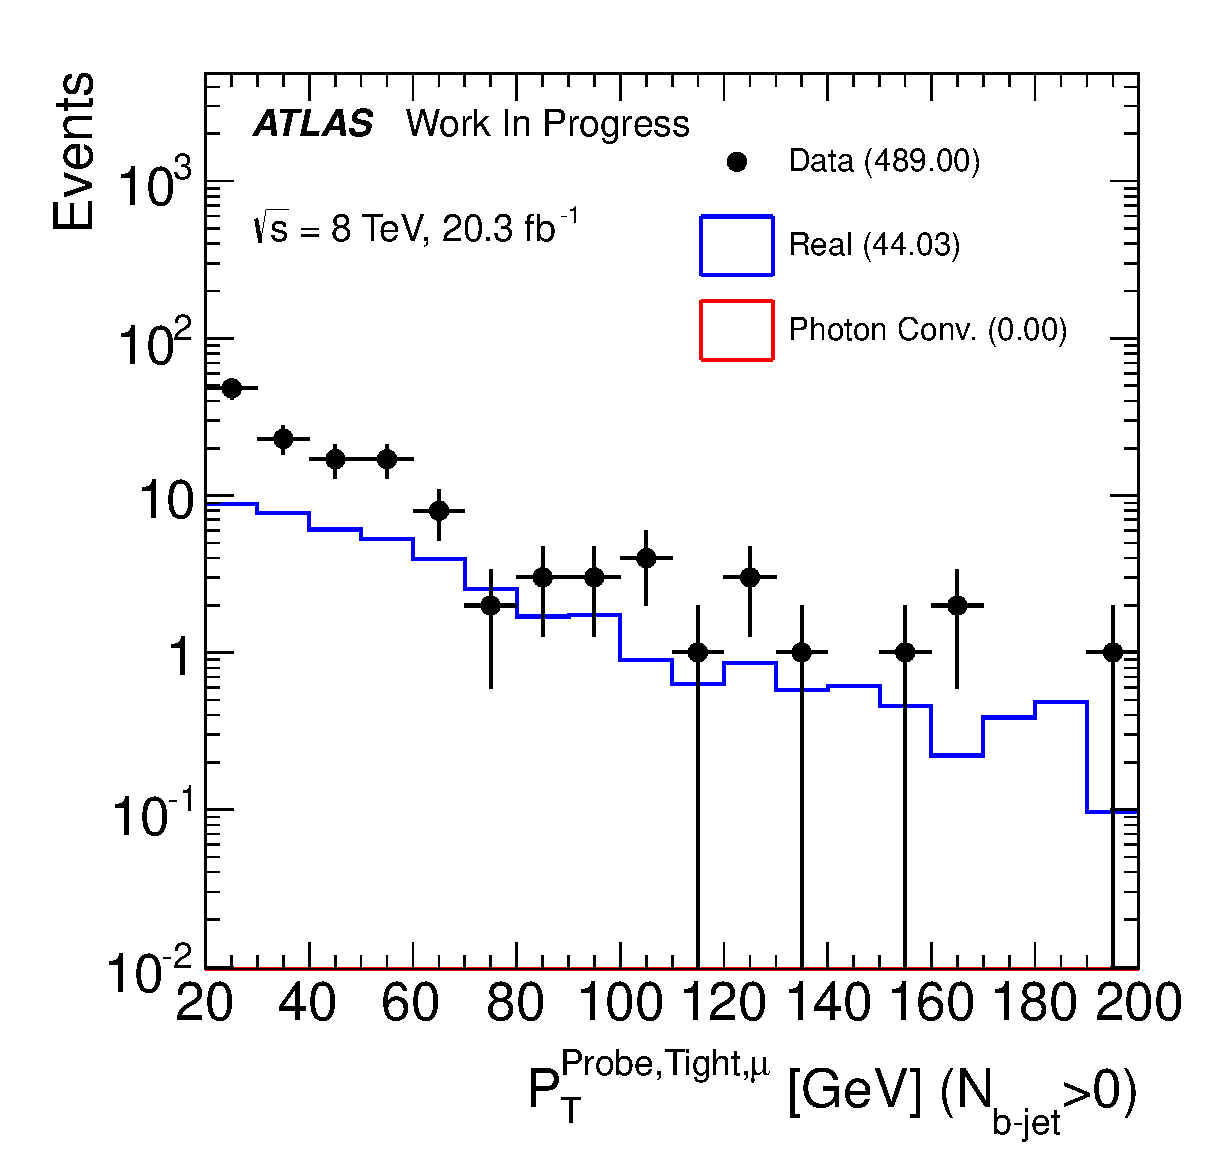
\includegraphics[width=0.45\columnwidth]{figures/fakes_bkg/CRs/SameSignMuonMuon/NoStack/ProbeTightMuonPtBJetGt0.eps}
}
%\vspace{-1mm}
\centering
\subfigure{
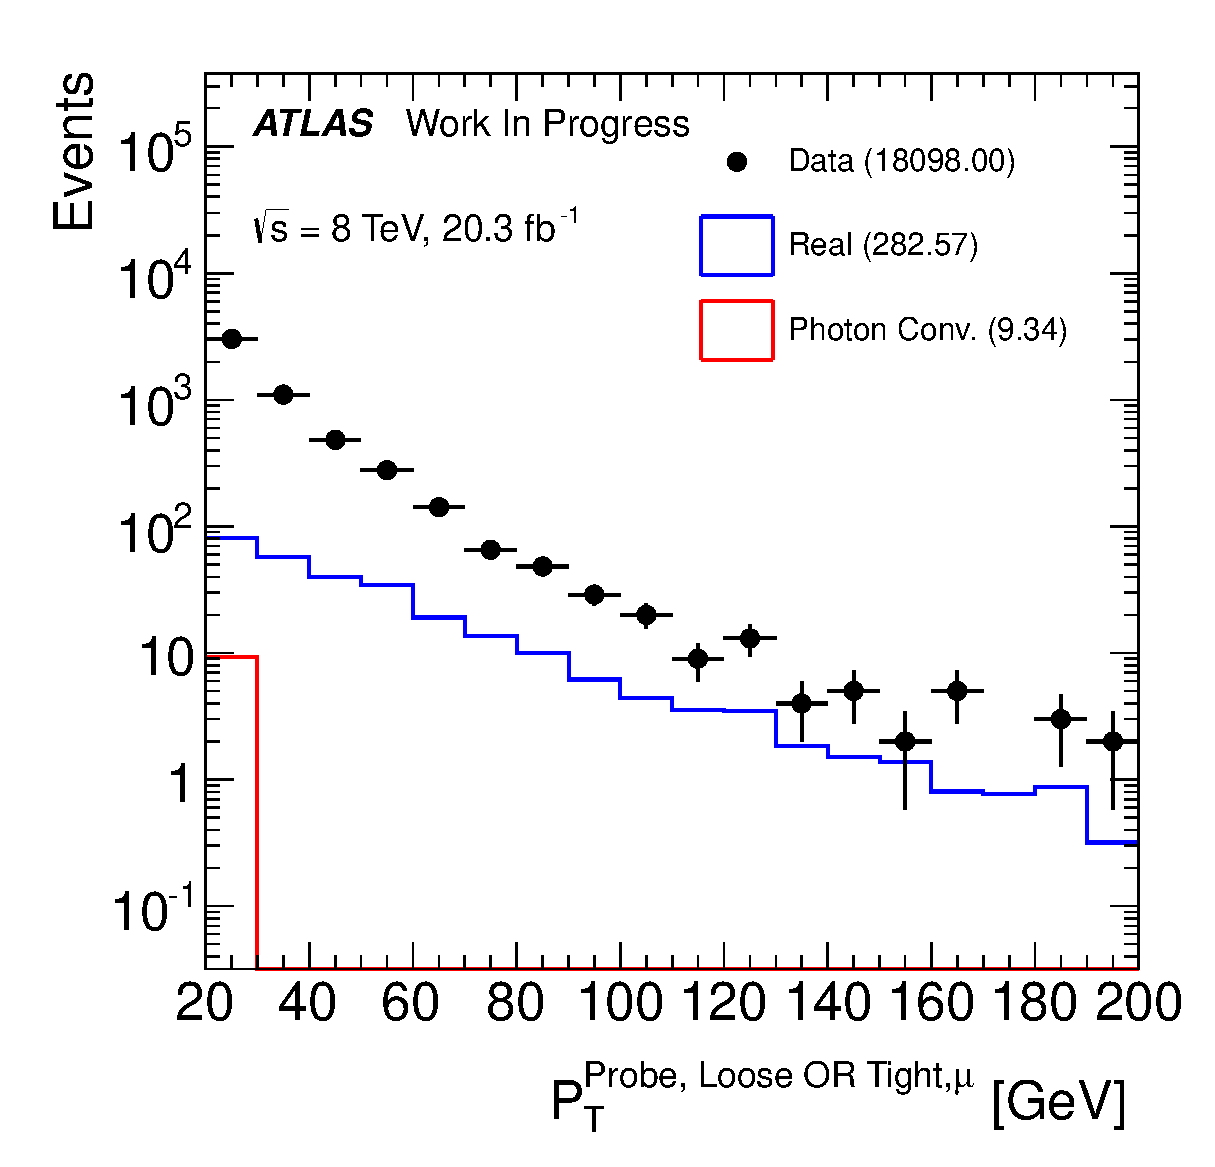
\includegraphics[width=0.45\columnwidth]{figures/fakes_bkg/CRs/SameSignMuonMuon/NoStack/ProbeLooseORTightMuonPt.eps}
}
%\centering
%\subfigure{
%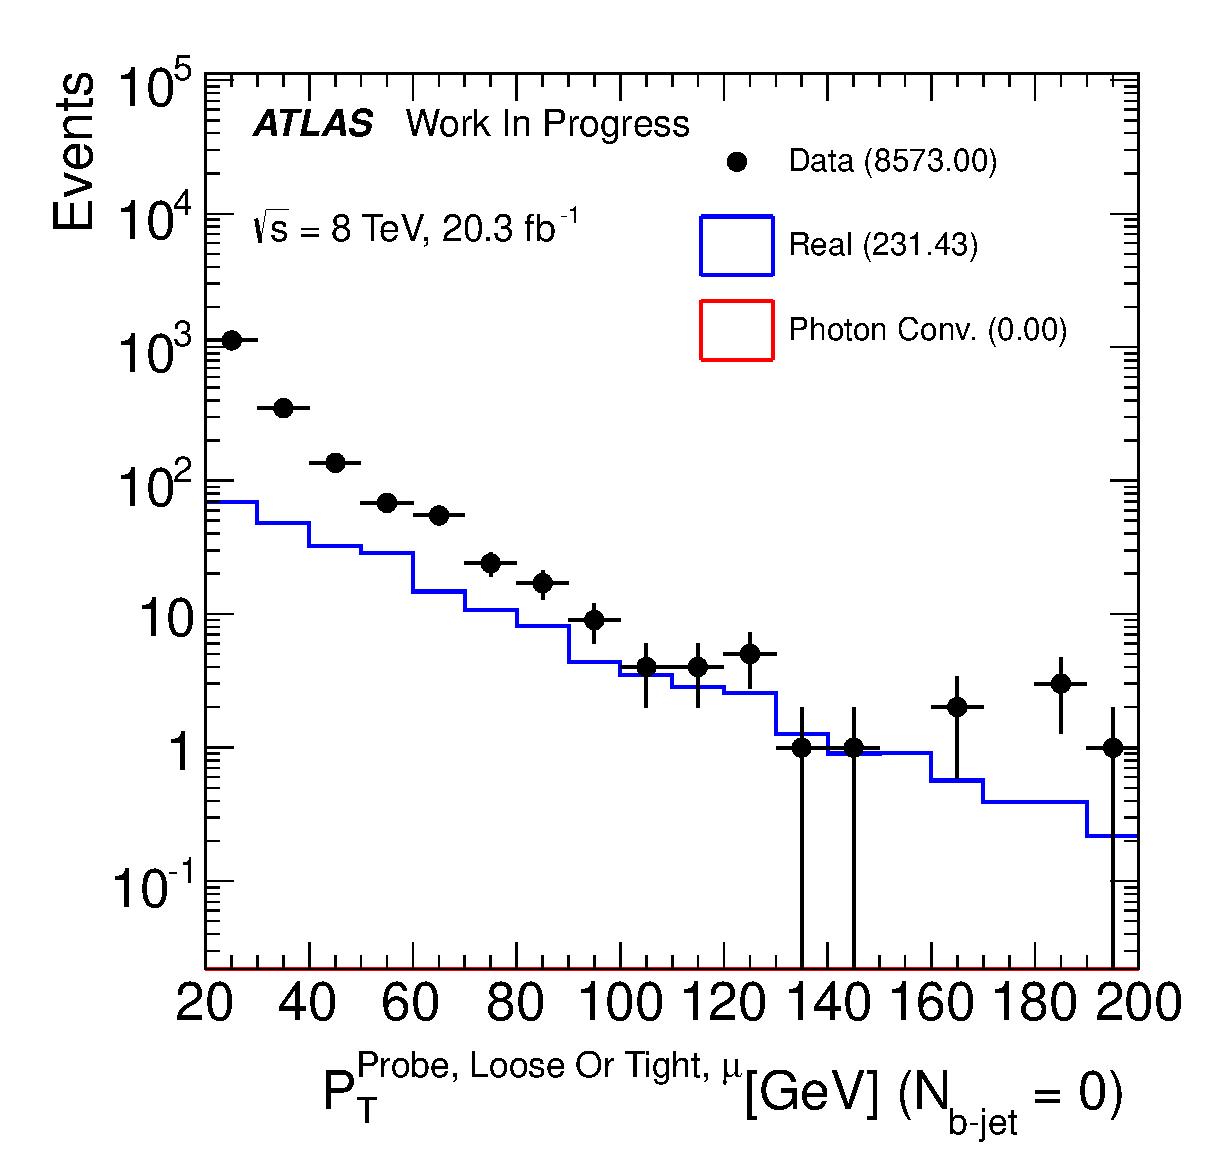
\includegraphics[width=0.45\columnwidth]{figures/fakes_bkg/CRs/SameSignMuonMuon/NoStack/ProbeLooseORTightMuonPtBJetEq0.eps}
%}
\centering
\subfigure{
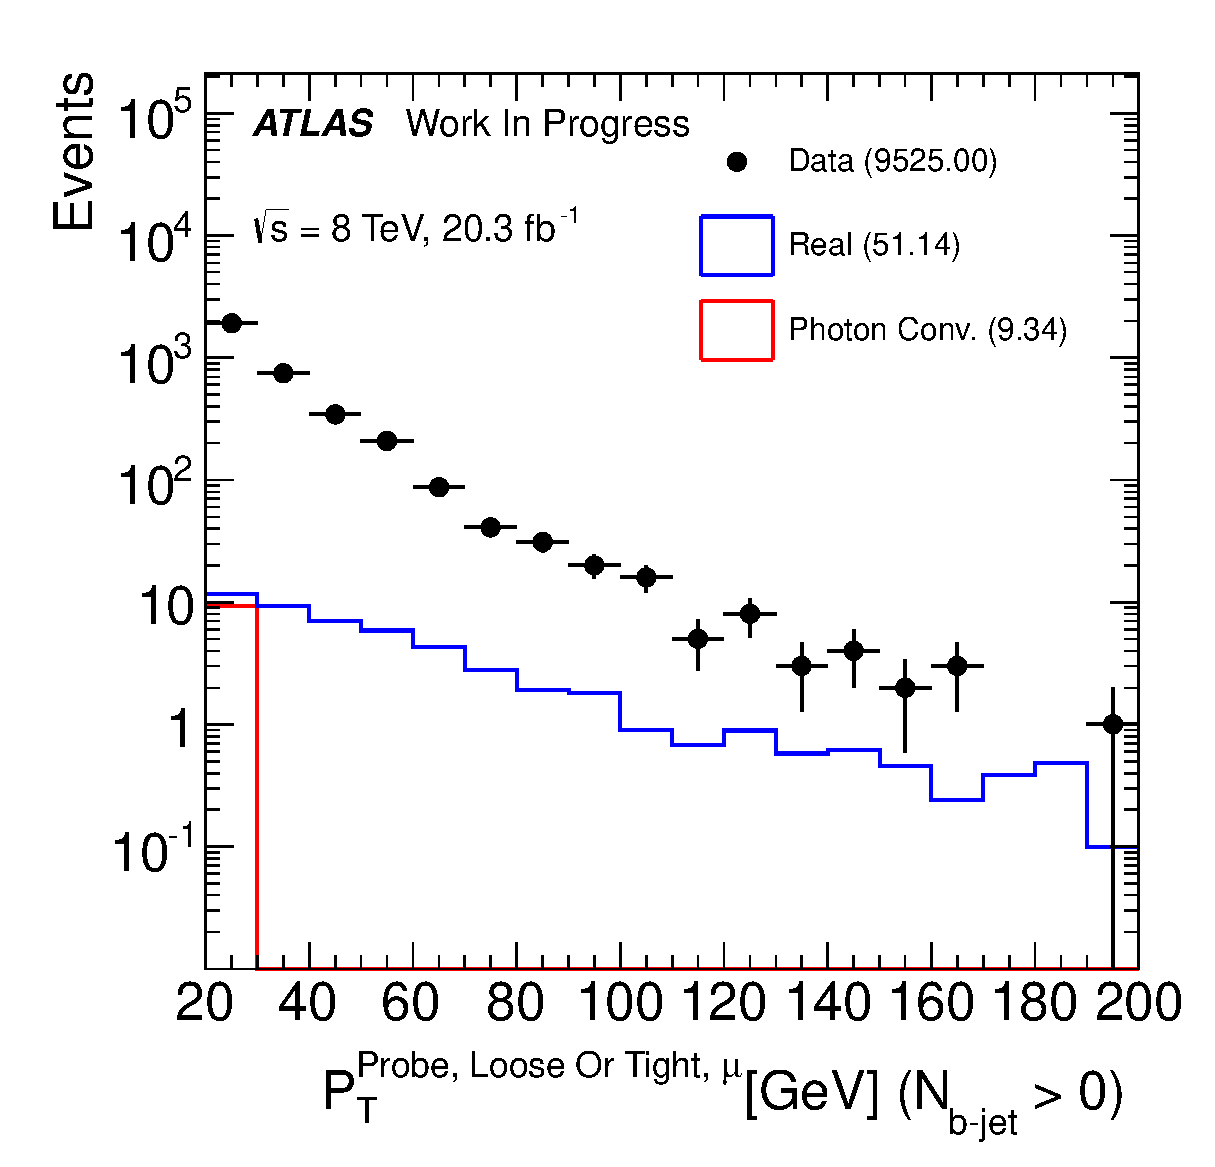
\includegraphics[width=0.45\columnwidth]{figures/fakes_bkg/CRs/SameSignMuonMuon/NoStack/ProbeLooseORTightMuonPtBJetGt0.eps}
}
\vspace{-10mm}\caption{Transverse momentum distributions \pt\ of tight probe muons (top) and loose OR tight probe muons (bottom) passing signal selection criteria in the control Same-Sign $\mu-\mu$ control region without any additional requirement on $b$-jets in the event (left) and at least one $b$-jet (right). 
The amount observed in data (black points) corresponds to $n$ (bottom) and $n_{\textrm{Tight}}$ (top) in Eq.~\ref{eq:fakerate}. 
Meanwhile, the contribution determined in MC to come from real leptons (blue line) and from photon conversion (red line) are shown 
separately; they are not stacked. The real lepton contribution corresponds to 
$n_{\textrm{Tight}}^{\textrm{Real}}$ (top) and $n^{\textrm{Real}}$ (bottom) and the photon conversion 
contribution corresponds to $n_{\textrm{Tight}}^{\textrm{PC}}$ (top) and $n^{\textrm{PC}}$ (bottom) in Eq.~\ref{eq:fakerate}. The photon conversion is 
observed to be negligible for muons.  }
\label{fig:fakeEff_CRs_muon}
\end{figure}

\begin{figure}[h!]
\centering
\subfigure{
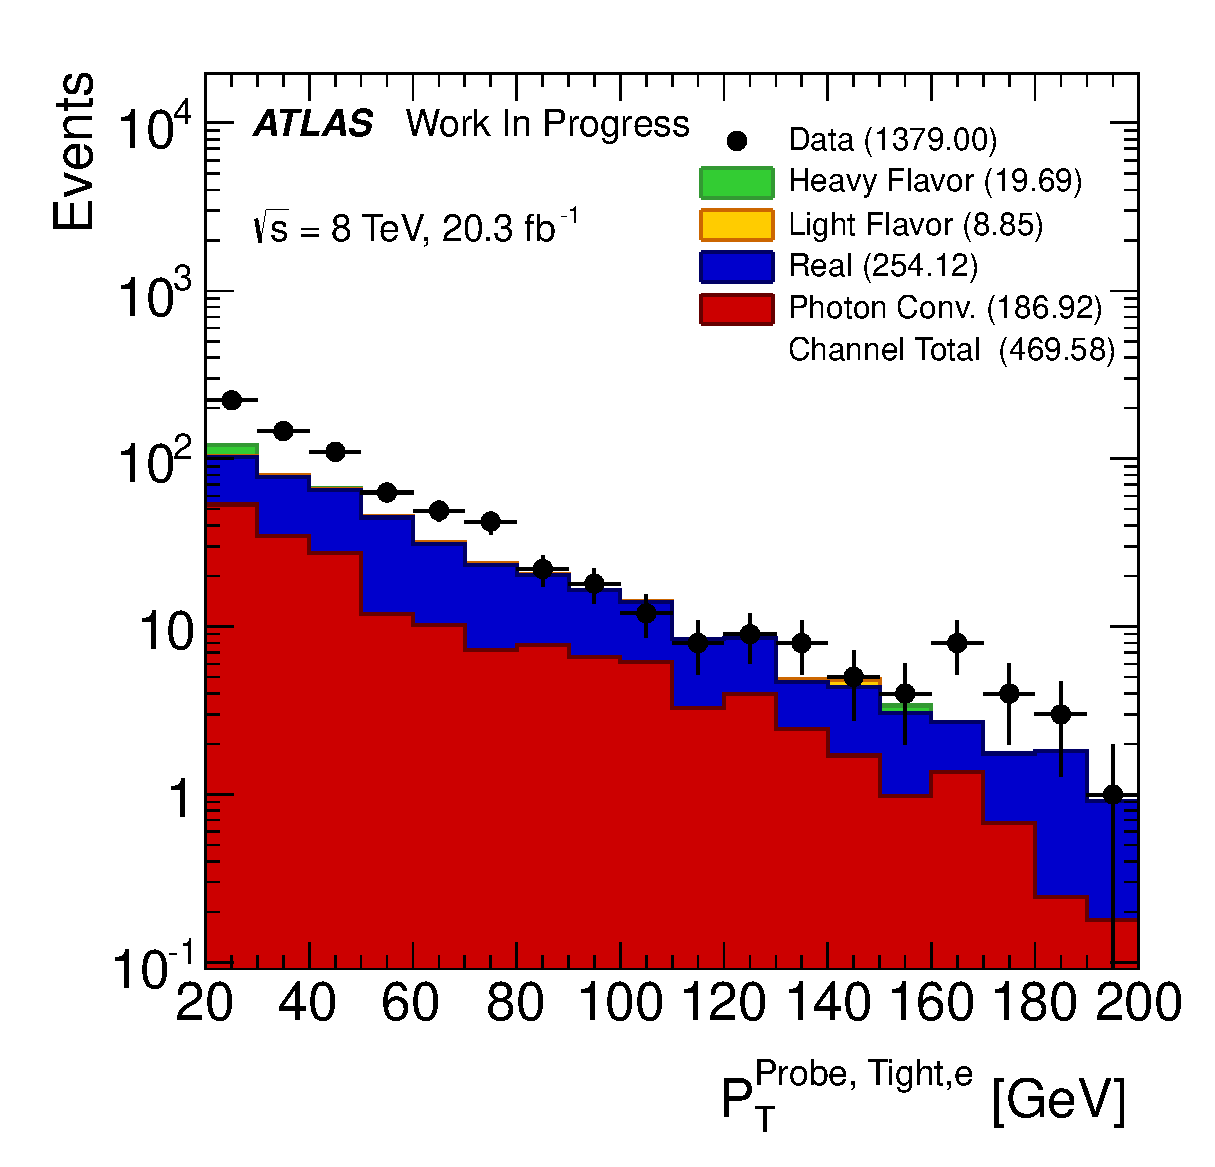
\includegraphics[width=0.45\columnwidth]{figures/fakes_bkg/CRs/SameSignElectronMuon/NoStack/ProbeTightElectronPt.eps}
}
%\centering
%\subfigure{
%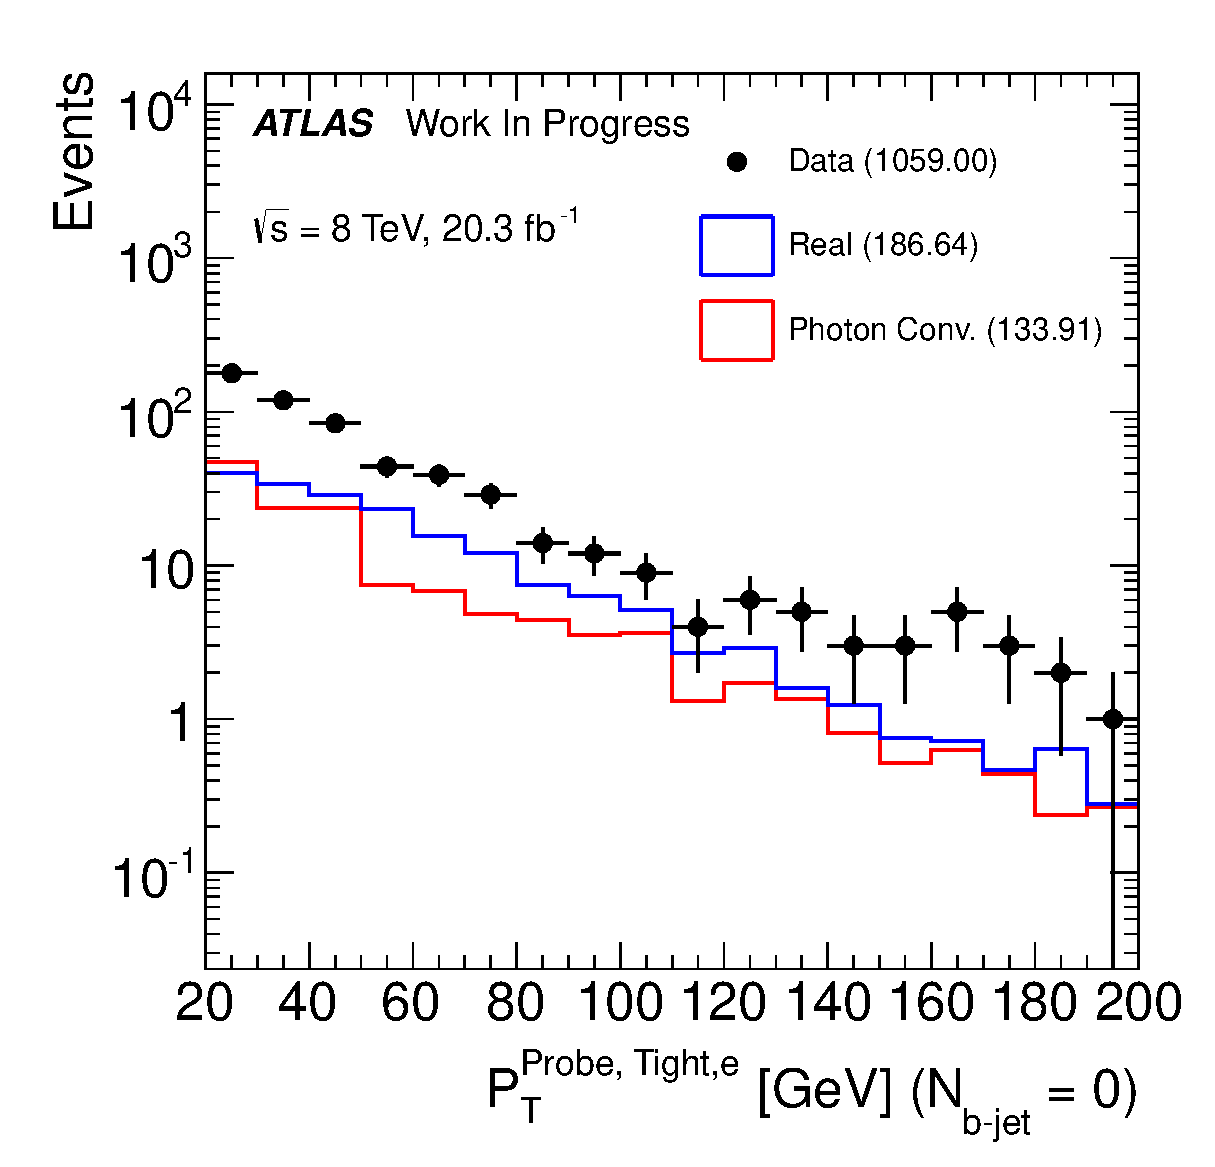
\includegraphics[width=0.3\columnwidth]{figures/fakes_bkg/CRs/SameSignElectronMuon/NoStack/ProbeTightElectronPtBJetEq0.eps}
%}
\centering
\subfigure{
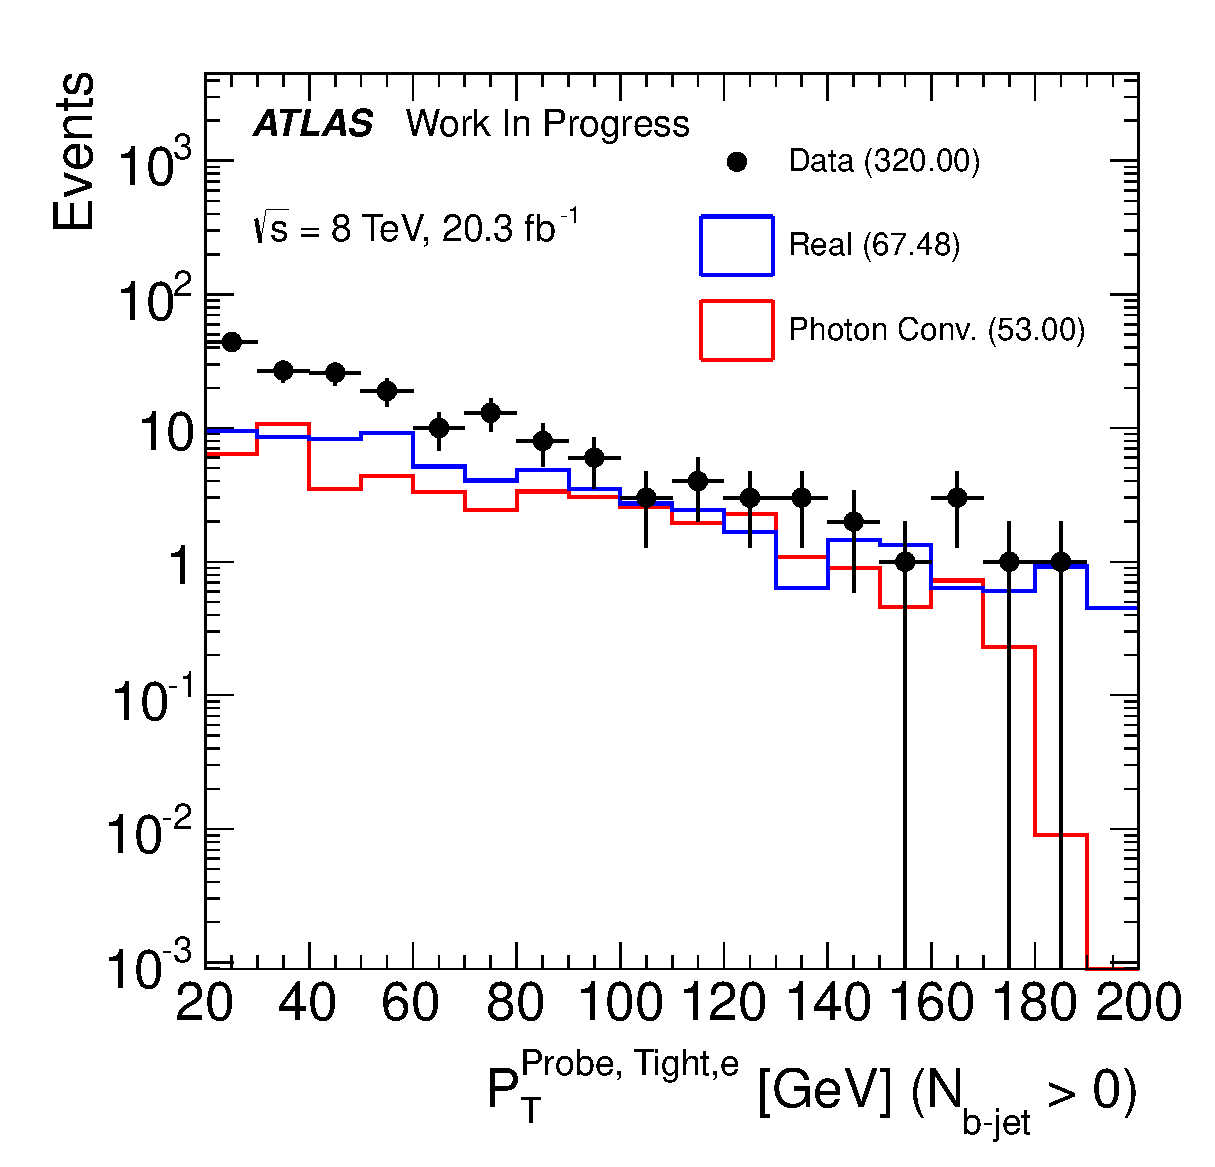
\includegraphics[width=0.45\columnwidth]{figures/fakes_bkg/CRs/SameSignElectronMuon/NoStack/ProbeTightElectronPtBJetGt0.eps}
}
\centering
\subfigure{
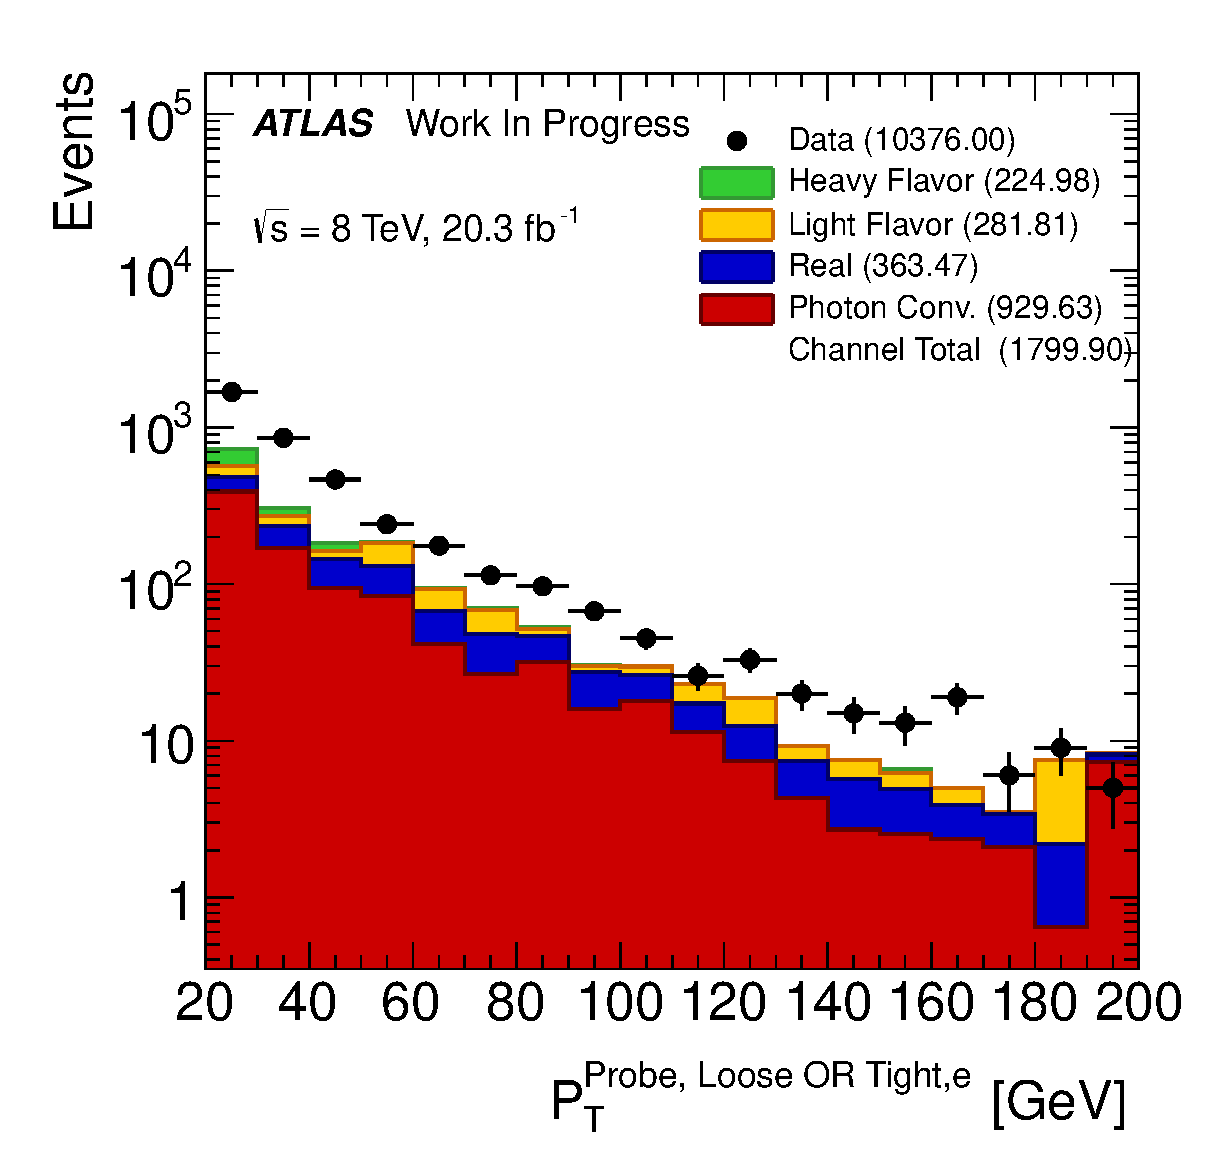
\includegraphics[width=0.45\columnwidth]{figures/fakes_bkg/CRs/SameSignElectronMuon/NoStack/ProbeLooseORTightElectronPt.eps}
}
%\centering
%\subfigure{
%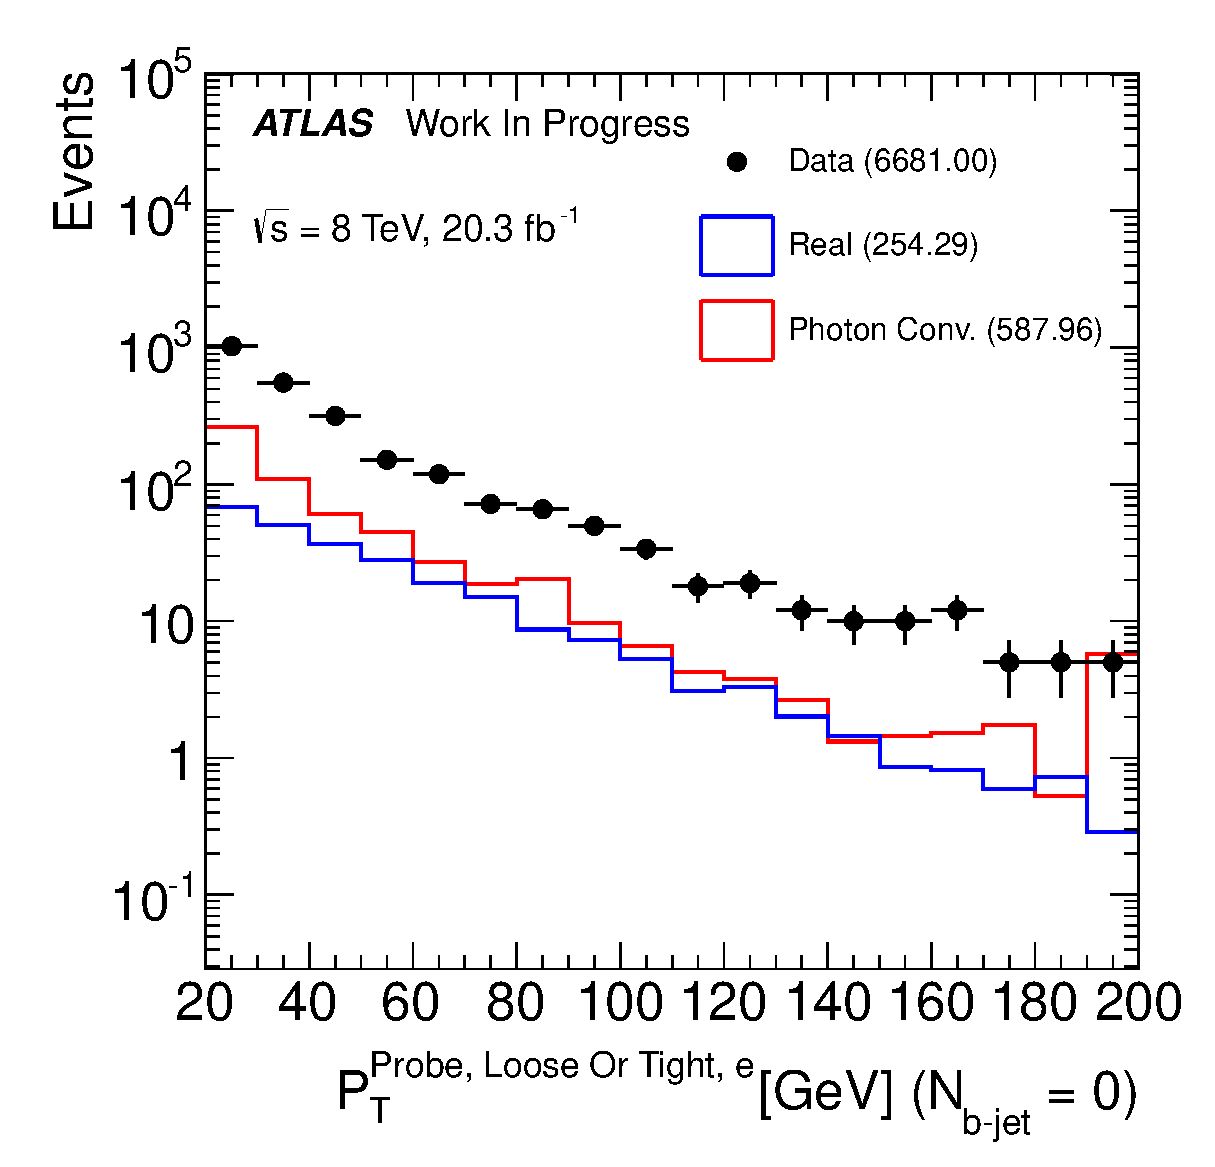
\includegraphics[width=0.3\columnwidth]{figures/fakes_bkg/CRs/SameSignElectronMuon/NoStack/ProbeLooseORTightElectronPtBJetEq0.eps}
%}
\centering
\subfigure{
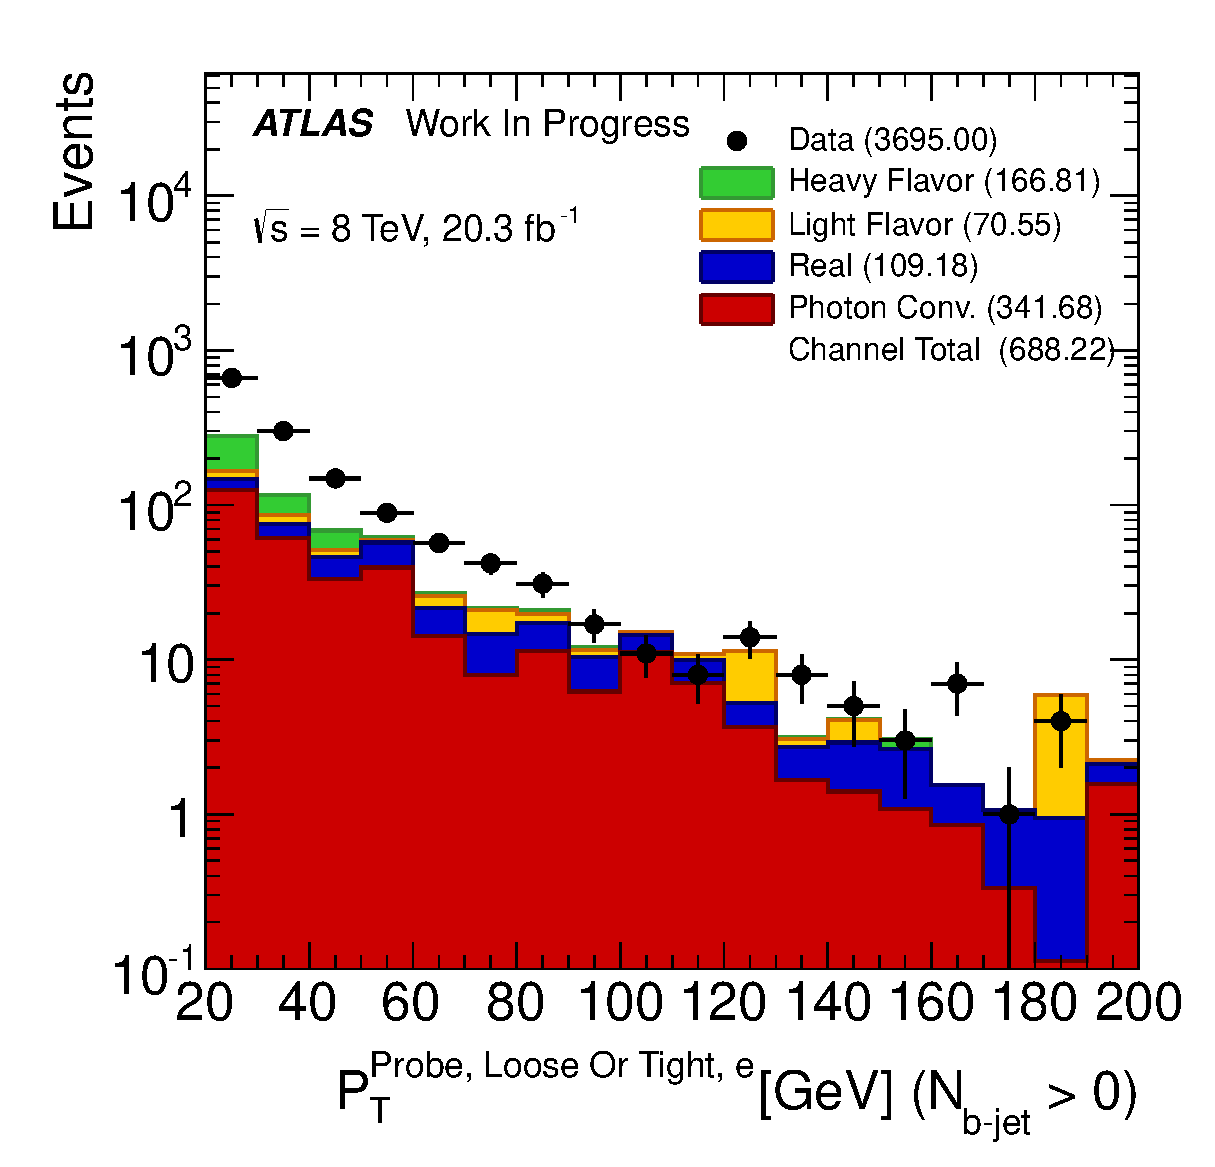
\includegraphics[width=0.45\columnwidth]{figures/fakes_bkg/CRs/SameSignElectronMuon/NoStack/ProbeLooseORTightElectronPtBJetGt0.eps}
}
%\vspace{-1mm}
\vspace{-10mm}\caption{Transverse momentum distributions \pt\ of tight probe electron (top) and loose or tight probe electrons (bottom) passing signal selection criteria in the Same-Sign $e-\mu$ control region without any additional requirement on $b$-jets in the event (left) and at least one $b$-jet (right).
The amount observed in data (black points) corresponds to $n$ (bottom) and $n_{\textrm{Tight}}$ (top) in Eq.~\ref{eq:fakerate}. 
Meanwhile, the contribution determined in MC to come from real leptons (blue line) and from photon conversion (red line) are shown 
separately; they are not stacked. The real lepton contribution corresponds to 
$n_{\textrm{Tight}}^{\textrm{Real}}$ (top) and $n^{\textrm{Real}}$ (bottom) and the photon conversion 
contribution corresponds to $n_{\textrm{Tight}}^{\textrm{PC}}$ (top) and $n^{\textrm{PC}}$ (bottom) in Eq.~\ref{eq:fakerate}.  }
\label{fig:fakeEff_CRs_electron}
\end{figure}






\begin{figure}[ht!]
\centering
\includegraphics[width=0.45\columnwidth]{figures/fakes_bkg/Efficiencies/ElectronFakeRates.png}
\includegraphics[width=0.45\columnwidth]{figures/fakes_bkg/Efficiencies/MuonFakeRates.png}
%\vspace{-10mm}
\caption{Distributions of the electron (left) and muon (right) fake rates as a function of \pt\ extracted in the control regions for three different selections: without any additional requirement on $b$-jets in the event and at least one $b$-jet.}
\label{fig:fakeEff}
\end{figure}




%\tabcolsep=0.1cm
%\begin{table}
%\centering
%\resizebox{0.8\textwidth}{!}{
%\begin{tabular}{l|c|c|c|c|c|c|c} 
%\hline
%\multicolumn{4}{c}{Electrons} &\multicolumn{4}{c}{Muons}\\ \hline
%\pt\ region & Fake eff. & $\sigma_{\mathrm{stat}}$ & $\sigma_{\mathrm{syst}}$ &\pt\ region & Fake eff. & $\sigma_{\mathrm{stat}}$ & $\sigma_{\mathrm{syst}}$ \\\hline
%$\pt \in [10, 15]$ \GeV\ & $0.$ & $0.$ & $0.$ 
%& $\pt \in [10, 15]$ \GeV\ & $0.$ & $0.$ & $0.$ \\
%$\pt \in [15, 30]$ \GeV\ & $0.$ & $0.$ & $0.$
%& $\pt \in [15, 20]$ \GeV\ & $0.$ & $0.$ & $0.$ \\
%$\pt\in [30, 50]$ \GeV\ & $0.$ & $0.$ & $0.$
%& $\pt\in [20, 40]$ \GeV\ & $0.$ & $0.$ & $0.$ \\
%$\pt > 50$ \GeV\ & $0.$ & $0.$ & $0.$
%& $\pt > 40$ \GeV\ & $0.$ & $0.$ & $0.$ \\
%\hline
%\end{tabular}  }
%\caption{Measured fake efficiencies for electrons and muons including statistical and systematic absolute uncertainties.} 
%\label{table:fakeEff_All}
%\end{table} 

\begin{table}[h]
\centering
\begin{tabular}{|l||c|c|c|c||c|c|c|c|}
\hline
 & $\zeta$ & $\sigma_{stat}$ & $\sigma_{sys}^{uncorr}$ & $\sigma_{sys}^{corr}$\\ 
\hline\hline
&\multicolumn{4}{c||}{$N_{b-jet} > 0$}\\ \hline
$p_{T}\in[20,30]$ GeV &  $0.0549$ &  $0.0136$ &  $0.0084$ &  $0.0032$\\ 
$p_{T}\in[30,50]$ GeV &  $0.0645$ &  $0.0272$ &  $0.0203$ &  $0.0161$\\ 
$p_{T} > 50$ GeV &  $0.0816$ &  $0.0723$ &  $0.0764$ &  $0.1088$\\ 
\hline\hline &\multicolumn{4}{c||}{$N_{b-jet} \geq 0$}\\ \hline
$p_{T}\in[20,30]$ GeV &  $0.0995$ &  $0.0141$ &  $0.0270$ &  $0.0099$\\ 
$p_{T}\in[30,50]$ GeV &  $0.1192$ &  $0.0208$ &  $0.0324$ &  $0.0232$\\ 
$p_{T} > 50$ GeV &  $0.1428$ &  $0.0374$ &  $0.0428$ &  $0.0674$\\ 
\hline
\end{tabular}

\caption{Measured fake efficiencies for electrons measured in three regions: with no additional requirements on the presence of $b$-jets and with at least one $b$-jet in a event. Statistical and systematic absolute uncertainties are also shown.} 
\label{table:fakeEff_El}
\end{table} 


\begin{table}[h]
\centering
\begin{tabular}{|l||c|c|c|c||c|c|c|c|}
\hline
 & $\zeta$ & $\sigma_{stat}$ & $\sigma_{sys}^{uncorr}$ & $\sigma_{sys}^{corr}$\\ 
\hline\hline
&\multicolumn{4}{c||}{$N_{b-jet} > 0$}\\ \hline
$p_{T}\in[20,30]$ GeV &  $0.0208$ &  $0.0037$ &  $0.0067$ &  $0.0009$\\ 
$p_{T}\in[30,40]$ GeV &  $0.0207$ &  $0.0066$ &  $0.0113$ &  $0.0020$\\ 
$p_{T} > 40$ GeV &  $0.0492$ &  $0.0109$ &  $0.0259$ &  $0.0068$\\ 
\hline\hline &\multicolumn{4}{c||}{$N_{b-jet} \geq 0$}\\ \hline
$p_{T}\in[20,30]$ GeV &  $0.0378$ &  $0.0046$ &  $0.0140$ &  $0.0040$\\ 
$p_{T}\in[30,40]$ GeV &  $0.0360$ &  $0.0091$ &  $0.0096$ &  $0.0089$\\ 
$p_{T} > 40$ GeV &  $0.0967$ &  $0.0166$ &  $0.0252$ &  $0.0244$\\ 
\hline
\end{tabular}

\caption{Measured fake efficiencies for muons measured in three regions: with no additional requirements on the presence of $b$-jets and with at least one $b$-jet in the event.  Statistical and systematic absolute uncertainties are also shown.} 
\label{table:fakeEff_Mu}
\end{table} 


\clearpage

\subsubsection{Study of the fake lepton composition}
\label{sec:fakecomposition}

The use of the generalized matrix method to determine the 
relies on the assumption that the 
fake rates derived in the di-lepton control regions may be extrapolated to the three lepton signal regions.  
The fake rate depends primarily on the source of the fake leptons, thus
one can check the validity of this assumption by looking at the composition of the
different fake lepton sources in the dilepton control regions and comparing 
them to the
composition in the three lepton signal regions. 

The fake composition is investigated by classifying the MC events as a function of the origin of the fake leptons found in each event.  The MCTruthClassifier tool~\cite{MCtruthclassifier:twiki} is used
to identify the fake laptops origin as follows:

\begin{itemize}
\item Real - Prompt leptons
		\begin{itemize}
		\item \emph{IsoElectron} 
		\item \emph{IsoMuon}
		\item In $Z\gamma$ events classified as either \emph{UnknownElectron} or \emph{UnknownMuon} and parent of lepton is $\gamma$.
		\item In $Z\rightarrow\tau\tau$ events classified as either \emph{NonIsoElectron} or \emph{NonIsoMuon} and lepton has $\tau$ as parent.
		\end{itemize}
\item Heavy Flavor (HF) - Leptons from heavy flavor jets or heavy hadron decays
		\begin{itemize}
		\item \emph{NonIsoElectron} 
		\item \emph{NonIsoMuon}
		\end{itemize}
\item Light Flavor (LF) -  Leptons from light flavor jets
		\begin{itemize}
		\item \emph{Hadron} 
		\item \emph{Others}
		\item In $ZWW$ and $ZZZ$ events classified as either \emph{UnknownElectron} or \emph{UnknownMuon} and parent of lepton is either an up quark, down quark, or a gluon.
		\end{itemize}
\item Photon Conversion (PC)  - Leptons due to radiation
		\begin{itemize}
		\item \emph{BkgElectron} 
		\item \emph{BkgMuon}
		\end{itemize}

\end{itemize}

The composition is shown for electrons in the dilepton control 
regions in Table~\ref{table:CompositionElectronCR} and in the event pre-selection and in region close to the signal regions in Table~\ref{table:CompositionElectronSR}.
First, one can see that the PC contribution is roughly half of the fake contribution
estimate using MC
in the control regions and in the region close to the signal regions. Since this is being estimated
using MC close to the signal regions, 
this component is subtracted out in order to remove any double counting
in the final estimate. Then, after subtraction,
if one compares the composition in the control regions
to the composition in the region close to the signal regions only for electrons, 
in particular after tight selection, one can see that 
the composition is similar for both, 
with about 50 to 75 \% coming from HF and the rest from LF.

For the muons, one can see the composition in the dilepton control regions in 
Table~\ref{table:CompositionMuonCR} and in the event pre-selection
and region close to the signal regions in Table~\ref{table:CompositionMuonSR}. For the muons the PC
component is negligible, as expected, and there is no need for subtraction.
In this case, the composition is dominated by HF, contributing about 90\% with the
rest coming from LF.  This is true in the region close to the signal regions and in the control regions.

The differences observed in the composition between the inclusive $b-jet$ and $b-jet$ 
tagged dilepton control regions is observed to be of a similar size
to the difference in the composition for the region close to the signal regions for both the electron 
and muon cases.
Thus, comparing the rates derived in the control regions using the two different
$b-jet$ criteria should take into account any differences in the composition due
to extrapolation. This is the motivation for choosing the difference in these two 
control regions as an additional systematic on the fake rates.

Using this study of the composition, we conclude that the composition appears to be
consistent between the control regions and the region close to the signal regions.  We have chosen 
a comparison of two different dilepton control regions to be used a systematic
which should take into account any remaining differences in the composition.

It should be said that in the dilepton control regions, 
the MC estimate strongly underestimates the amount observed
in data, presumably because of additional sources of fakes 
not modeled in our MC, such as from QCD. 
The difference in the estimates can be clearly seen in Figures~\ref{fig:fakeEff_CRs_muon_stacked}
and \ref{fig:fakeEff_CRs_electron_stacked} which show the stacked MC estimate from real, photon conversion,
heavy flavor and light flavor sources compared to data.
Thus, the composition estimates shown are only reliable 
if these additional sources would have a similar composition to the ones observed
in this study that we are able to model. This effectively 
puts a large uncertainty on the composition estimates observed in this study. Also,
because the additinonal sources are most likely dominated by QCD, the PC 
contribution to these sources should be small. Thus, the PC component before subtraction
is likely overstated as shown in 
Tables~\ref{table:CompositionElectronCR} 
and \ref{table:CompositionElectronSR}.
As discussed earlier, we subtract the PC
component from the data when obtaining the fake rate. This procedure then assumes
explicitly that all of the photon conversion contribution is modeled in MC and is 
small.


\begin{figure}[h!]
\centering
\subfigure{
\includegraphics[width=0.45\columnwidth]{figures/fakes_bkg/CRs/SameSignMuonMuon/Stacked/ProbeTightMuonPt.eps}
}
%\centering
%\subfigure{
%\includegraphics[width=0.3\columnwidth]{figures/fakes_bkg/CRs/SameSignMuonMuon/Stacked/ProbeTightMuonPtBJetEq0.eps}
%}
\centering
\subfigure{
\includegraphics[width=0.45\columnwidth]{figures/fakes_bkg/CRs/SameSignMuonMuon/Stacked/ProbeTightMuonPtBJetGt0.eps}
}
%\vspace{-1mm}
\centering
\subfigure{
\includegraphics[width=0.45\columnwidth]{figures/fakes_bkg/CRs/SameSignMuonMuon/Stacked/ProbeLooseORTightMuonPt.eps}
}
%\centering
%\subfigure{
%\includegraphics[width=0.45\columnwidth]{figures/fakes_bkg/CRs/SameSignMuonMuon/Stacked/ProbeLooseORTightMuonPtBJetEq0.eps}
%}
\centering
\subfigure{
\includegraphics[width=0.45\columnwidth]{figures/fakes_bkg/CRs/SameSignMuonMuon/Stacked/ProbeLooseORTightMuonPtBJetGt0.eps}
}
\vspace{-10mm}\caption{Transverse momentum distributions \pt\ of tight probe muons (top) and loose OR tight probe muons (bottom) passing signal selection criteria in the control Same-Sign $\mu-\mu$ control region without any additional requirement on $b$-jets in the event (left) and at least one $b$-jet (right). 
The amount observed in data (black points) corresponds to $n$ (bottom) and $n_{\textrm{Tight}}$ (top) in Eq.~\ref{eq:fakerate}. 
Meanwhile, the contribution determined in MC to come from real leptons (blue), photon conversion (red), heavy flavor (green) and light
flavor (orange) are shown stacked on top of each other. 
The difference between the data and MC does not effect the data-driven
fake estimate but may have an impact on the composition estiamte.
}
\label{fig:fakeEff_CRs_muon_stacked}
\end{figure}

\begin{figure}[h!]
\centering
\subfigure{
\includegraphics[width=0.45\columnwidth]{figures/fakes_bkg/CRs/SameSignElectronMuon/Stacked/ProbeTightElectronPt.eps}
}
%\centering
%\subfigure{
%\includegraphics[width=0.3\columnwidth]{figures/fakes_bkg/CRs/SameSignElectronMuon/Stacked/ProbeTightElectronPtBJetEq0.eps}
%}
\centering
\subfigure{
\includegraphics[width=0.45\columnwidth]{figures/fakes_bkg/CRs/SameSignElectronMuon/Stacked/ProbeTightElectronPtBJetGt0.eps}
}
\centering
\subfigure{
\includegraphics[width=0.45\columnwidth]{figures/fakes_bkg/CRs/SameSignElectronMuon/Stacked/ProbeLooseORTightElectronPt.eps}
}
%\centering
%\subfigure{
%\includegraphics[width=0.3\columnwidth]{figures/fakes_bkg/CRs/SameSignElectronMuon/Stacked/ProbeLooseORTightElectronPtBJetEq0.eps}
%}
\centering
\subfigure{
\includegraphics[width=0.45\columnwidth]{figures/fakes_bkg/CRs/SameSignElectronMuon/Stacked/ProbeLooseORTightElectronPtBJetGt0.eps}
}
%\vspace{-1mm}
\vspace{-10mm}\caption{Transverse momentum distributions \pt\ of tight probe electron (top) and loose or tight probe electrons (bottom) passing signal selection criteria in the Same-Sign $e-\mu$ control region without any additional requirement on $b$-jets in the event (left) and at least one $b$-jet (right).
The amount observed in data (black points) corresponds to $n$ (bottom) and $n_{\textrm{Tight}}$ (top) in Eq.~\ref{eq:fakerate}. 
Meanwhile, the contribution determined in MC to come from real leptons (blue), photon conversion (red), heavy flavor (green) and light
flavor (orange) are shown stacked on top of each other.
The difference between the data and MC does not effect the data-driven
fake estimate but may have an impact on the composition estiamte.
}
\label{fig:fakeEff_CRs_electron_stacked}
\end{figure}

%%%%%%%%%%%scaled

%\begin{figure}[h!]
%\centering
%\subfigure{
%\includegraphics[width=0.45\columnwidth]{figures/fakes_bkg/CRs/SameSignMuonMuon/Scaled/coarse/ProbeTightMuonPtFakeRate_histratio.png}
%}
%\centering
%\subfigure{
%\includegraphics[width=0.45\columnwidth]{figures/fakes_bkg/CRs/SameSignMuonMuon/Scaled/coarse/ProbeTightMuonPtBJetGt0FakeRate_histratio.png}
%}
%\centering
%\subfigure{
%\includegraphics[width=0.45\columnwidth]{figures/fakes_bkg/CRs/SameSignMuonMuon/Scaled/coarse/ProbeLooseORTightMuonPtFakeRate_histratio.png}
%}
%\centering
%\subfigure{
%\includegraphics[width=0.45\columnwidth]{figures/fakes_bkg/CRs/SameSignMuonMuon/Scaled/coarse/ProbeLooseORTightMuonPtBJetGt0FakeRate_histratio.png}
%}
%\vspace{-10mm}\caption{Scaled....Transverse momentum distributions \pt\ of tight probe muons (top) and loose OR tight probe muons (bottom) passing signal selection criteria in the control Same-Sign $\mu-\mu$ control region without any additional requirement on $b$-jets in the event (left) and at least one $b$-jet (right). 
%The amount observed in data (black points) corresponds to $n$ (bottom) and $n_{\textrm{Tight}}$ (top) in Eq.~\ref{eq:fakerate}. 
%Meanwhile, the contribution determined in MC to come from real leptons (blue), photon conversion (red), heavy flavor (green) and light
%flavor (orange) are shown stacked on top of each other. 
%The difference between the data and MC does not effect the data-driven
%fake estimate but may have an impact on the composition estiamte.
%}
%\label{fig:fakeEff_CRs_muon_stacked_scaled}
%\end{figure}

%\begin{figure}[h!]
%\centering
%\subfigure{
%\includegraphics[width=0.45\columnwidth]{figures/fakes_bkg/CRs/SameSignElectronMuon/Scaled/coarse/ProbeTightElectronPtFakeRate_histratio.png}
%}
%\centering
%\subfigure{
%\includegraphics[width=0.45\columnwidth]{figures/fakes_bkg/CRs/SameSignElectronMuon/Scaled/coarse/ProbeTightElectronPtBJetGt0FakeRate_histratio.png}
%}
%\centering
%\subfigure{
%\includegraphics[width=0.45\columnwidth]{figures/fakes_bkg/CRs/SameSignElectronMuon/Scaled/coarse/ProbeLooseORTightElectronPtFakeRate_histratio.png}
%}
%\centering
%\subfigure{
%\includegraphics[width=0.45\columnwidth]{figures/fakes_bkg/CRs/SameSignElectronMuon/Scaled/coarse/ProbeLooseORTightElectronPtBJetGt0FakeRate_histratio.png}
%}
%\vspace{-10mm}\caption{Scaled...Transverse momentum distributions \pt\ of tight probe electron (top) and loose or tight probe electrons (bottom) passing signal selection criteria in the Same-Sign $e-\mu$ control region without any additional requirement on $b$-jets in the event (left) and at least one $b$-jet (right).
%The amount observed in data (black points) corresponds to $n$ (bottom) and $n_{\textrm{Tight}}$ (top) in Eq.~\ref{eq:fakerate}. 
%Meanwhile, the contribution determined in MC to come from real leptons (blue), photon conversion (red), heavy flavor (green) and light
%flavor (orange) are shown stacked on top of each other.
%The difference between the data and MC does not effect the data-driven
%fake estimate but may have an impact on the composition estiamte.
%}
%\label{fig:fakeEff_CRs_electron_stacked_scaled}
%\end{figure}


\begin{table}[ht!]
\centering
\begin{tabular}{|lc|ccc|}
    \hline
    \multicolumn{5}{|c|}{\bf{Control regions}}   \\ \hline \hline
    PC subtracted &$N_{b-jet}$  &{HF} &{PC} &{LF} \\ \hline
    yes &--- &$57\pm 4$\%  &$0$\% &$43\pm 6$\% \\
    yes &$N_{b-jet}>0$  &$75\pm 5$\% &$0$\% &$25\pm 3$\% \\ \hline
    no &--- &$22\pm 3$\% &$61\pm 13$\% &$17\pm 3$\% \\
    no &$N_{b-jet}>0$  &$43\pm 3$\% &$42\pm 6$\% &$15\pm 2$\% \\ 
    \hline
	
\end{tabular}




\caption{
Composition of fake electrons taken from  MC events in the same-sign electron-muon dilepton control regions
used to extract electron fake rates. The composition is split as either Heavy Flavor (HF), Photon
Conversion (PC), and Light Flavor (LF) are shown. In the ``PC subtracted'' case, the PC component
has been explicitly removed.  This corresponds to the scenario ultimately used in the
fake rate estimation.
}
\label{table:CompositionElectronCR}
\end{table}

\begin{table}[ht!]
\centering
    \begin{tabular}{|l||cc|}
    \hline 
    \multicolumn{3}{|c|}{\bf{Pre-selection and signal regions}}   \\ 
    & Heavy Flavor & Light Flavor \\
    \hline \hline
    \hline

    Pre-selection &$53.7 \pm 9.4$\% & $46.3\pm 10.0$\% \\
    0 SFOS &$80.2 \pm 19.9$\% & $19.8\pm 11.8$\% \\
    1 SFOS &$52.4 \pm 12.5$\% & $47.6\pm 11.9$\% \\
    2 SFOS &$47.7 \pm 16.1$\% & $52.3\pm 23.3$\% \\
    \hline


  \end{tabular}
  








\caption{
Composition of fake electrons taken from  MC events in the event pre-selection and regions close to the signal regions used in the analysis. 
The composition is split as either Heavy Flavor (HF) or Light Flavor (LF). 
}
\label{table:CompositionElectronSR}
\end{table}


\begin{table}[ht!]
\centering
    \begin{tabular}{|lc|ccc|}
    \hline
    \multicolumn{5}{|c|}{\bf{Control regions}}   \\ \hline \hline
    PC subtracted &$N_{b-jet}$  &{HF} &{PC} &{LF} \\ \hline
    yes &--- &$89\pm 4$\% &$0$\% &$11\pm 1$\% \\
    yes &$N_{b-jet}>0$  &$95\pm 3$\% &$0$\% &$4\pm 1$\%\\ \hline
    no &--- &$89\pm 4$\% &$0$\% &$11\pm 1$\% \\
    no &$N_{b-jet}>0$  &$95\pm 3$\% &$0$\% &$4\pm 1$\%\\ 
    %\color{yellow!70!black}\met\ $>10$GeV &\color{yellow!70!black}$N_{b-jet}>1$  &\color{yellow!70!black}91\% &\color{yellow!70!black}0\% &\color{yellow!70!black}9\% \\ 
    \hline
  \end{tabular}
  

\caption{
Composition of fake muons taken from  MC events in the event pre-selection and regions close to the signal regions used in the analysis. 
The composition is split as either Heavy Flavor (HF), Photon
Conversion (PC), and Light Flavor (LF) are shown. The photon conversion component
is measured to be negligible. No PC subtraction is performed.
}
\label{table:CompositionMuonCR}
\end{table}

\begin{table}[ht!]
\centering
    \begin{tabular}{|l||cc|}
    \hline 
    \multicolumn{3}{|c|}{\bf{Pre-selection and signal regions}}   \\ 
    & Heavy Flavor & Light Flavor \\
    \hline \hline
    \hline

    Pre-selection &$78.9 \pm 10.0$\% & $21.1\pm 4.6$\% \\
    0 SFOS &$96.7 \pm 21.0$\% & $3.3\pm 3.7$\% \\
    1 SFOS &$77.4 \pm 14.1$\% & $22.6\pm 7.2$\% \\
    2 SFOS &$77.3 \pm 15.9$\% & $22.8\pm 7.1$\% \\
    \hline


  \end{tabular}
  








\caption{
Composition of fake muons taken from  MC events in the same-sign muon-muon dilepton control regions
used to extract the muon fake rates. The composition is split into either Heavy Flavor (HF) or Light Flavor (LF). 
}
\label{table:CompositionMuonSR}
\end{table}

\clearpage
\subsubsection{Fake lepton background validation}

A Monte Carlo closure test of the generalized matrix method is performed. The fake rates are computed from MC samples in the dilepton control regions defined in section~\ref{sec:fakecomposition}, and the method is then applied on the most important MC samples contributing to the event pre-selection: $Z$+jets and $t\bar{t}$. The event pre-selection is used for this test, because the statistics available for the MC samples containing fake leptons in the signal region is too small to be able to draw any conclusion. Figure~\ref{fig:MCFakeRatesClosure}, show the MC fake rates obtained from the CR, while figure~\ref{fig:MCClosureCheckMatrixMethod} show the MC agreement with the MC events reweighted using the generalized matrix method in the event pre-selection region, for the third-leading lepton $\pt$ and the $\met$ distribution. As it can be seen the shape agreement and the overall normalization are pretty good, showing that the matrix method is performing well.

\begin{figure}[ht!]
\centering
\includegraphics[width=0.42\columnwidth]{figures/ClosureCheck_MatrixMethod/ElFakeRates_MC_topZjets_new.pdf}
\includegraphics[width=0.42\columnwidth]{figures/ClosureCheck_MatrixMethod/MuFakeRates_MC_topZjets_new.pdf}
\caption{Distribution of the fake rates obtained from MC samples in the dilepton control regions. The errors shown here are statistical only. These rates are used to performed a MC closure check of the global matrix method.}
\label{fig:MCFakeRatesClosure}
\end{figure}

\begin{figure}[ht!]
\centering
\includegraphics[width=0.42\columnwidth]{figures/ClosureCheck_MatrixMethod/PtThirdLepSignal_TTT_total_new.pdf}
\includegraphics[width=0.42\columnwidth]{figures/ClosureCheck_MatrixMethod/VR_PMET_lepTTT_total_new.pdf}
\caption{Distributions of the third leading lepton $\pt$ and $\met$ in the event pre-selection region, for $Z$+jets and $t\bar{t}$, compared to events from these samples reweigthed using the global matrix method and the rates shown in Figure~\ref{fig:MCFakeRatesClosure}. Good agreement is observed}
\label{fig:MCClosureCheckMatrixMethod}
\end{figure}




The ability of the generalized matrix method just described to model accurately
the fake lepton background is tested in a control region designed to be enhanced
in the fake lepton background while mainitaining orthogonality with the signal
regions described in Section~\ref{sec:signal_regions}. The control region 
starts by using the event pre-selection region described in Section~\ref{sec:preselection}. To reduce contamination in the 
control region from the $WZ$ process, it is required that none
of the three leptons selected form a Same-Flavor Opposite-Sign lepton pair.
Finally, to ensure orthogonality with the signal regions which require that no
$b$-tagged jets are present in the event, this control region requires
the presence of at least one $b$-tagged jet in the event. 

This control region
is clearly dominated by the data-driven fake lepton background as can
be seen in Fig.~\ref{fig:FakeCR} and in Table~\ref{tab:FakeCR}. 
Furthermore, Table~\ref{tab:FakeCR} shows good agreement between data
and the fake background modeling on the total event yield, which is within 
the statistical uncertainties.  One can even see from
Fig.~\ref{fig:FakeCR} that the shape description does a reasonable job,
although the statistical uncertainty is a bit too large to draw strong conclusions.
One can also see that the systematic uncertainty easily covers most
of the differences that are observed. Thus, we conclude that the fake background
description is working and may be used in our signal regions.  Especially since
the fake background is most important in the 0 SFOS region (described in more
detail in Section~\ref{sec:signal_regions}) which differs primarily from this
control region only by the $b$-veto requirement.




\begin{figure}[ht!]
\centering
\includegraphics[width=0.3\columnwidth]{figures/Fake_CR/LeadingLeptonPt_histratio.eps}
\includegraphics[width=0.3\columnwidth]{figures/Fake_CR/SubleadingLeptonPt_histratio.eps}
\includegraphics[width=0.3\columnwidth]{figures/Fake_CR/MinimumLeptonPt_histratio.eps}
\includegraphics[width=0.3\columnwidth]{figures/Fake_CR/MET_Et_histratio.eps}
\includegraphics[width=0.3\columnwidth]{figures/Fake_CR/NBTaggedJets_histratio.eps}
\includegraphics[width=0.3\columnwidth]{figures/Fake_CR/NJets_histratio.eps}
\includegraphics[width=0.3\columnwidth]{figures/Fake_CR/NMuons_histratio.eps}
\caption{Distributions in a control region designed to study the data-driven fake lepton background estimate.  The selection used is as follows: Event pre-selection + 0 SFOS + at least 1 $b$-jet.  Good agreement is observed}
\label{fig:FakeCR}
\end{figure}

\begin{table}[ht!]
\centering
\begin{tabular}{|c||c|c|c|c|}
\hline
 & Event Yield\\ 
\hline\hline
$WZ$ &  $0.338 \pm 0.021$\\ 
$ZZ$ &  $0.0747 \pm 0.0064$\\ 
$Z\gamma$ &  $0.0058 \pm 0.0058$\\ 
$ZWW+ZZZ$ &  $0.026 \pm 0.005$\\ 
$t\bar{t}+V$ &  $3.228 \pm 0.039$\\ 
Fake (data-driven) &  $10.91 \pm 0.73$\\ 
$WWW$ &  $0.1431 \pm 0.0052$\\ 
\hline
Expected Background &  $14.58 \pm 0.73$\\ 
Expected Signal + Background &  $14.72 \pm 0.73$\\ 
\hline
Observed Data &  $18$\\ 
\hline
\end{tabular}

\caption{Expected and observed yields for the fake lepton control region.}
\label{tab:FakeCR}
\end{table}




Details of the MC based background estimations are described below.
Any additional normalizations or uncertainties are summarized
in Table~\ref{tab:mcnorm}.

\begin{table}[htp]
\centering
    \begin{tabular}{|c|cc|}
    \hline
    Background & Normalization Factor & Uncertainty \\ 
    \hline\hline
    $WZ$ & 1.08 & 10~\% \\
    $ZZ$ & 1.05 & 15~\% \\
    %$Z\gamma$ & & 30~\% \\
    $\ttbar +V$ & 1.0 & 30~\% \\
    $ZWW+ZZZ$ & 1.0 & 50~\% \\
    \hline
  \end{tabular}
  

\caption{Summary of normalizations and their uncertainties for the
MC based background estimates used in the analysis.}
\label{tab:mcnorm}
\end{table}



\subsubsection{$WZ$ Background}
\label{sec:wzbg}

The $WZ$ background is the most important prompt background 
to the $WWW$ signal process. Thus, it must be studied carefully.
The most recent measurements of the $WZ$ process at the LHC
\cite{Aad:2012twa,Anger:1663539,CMS-PAS-SMP-12-006} 
show some tension with the current NLO MC predictions for this process, 
with differences of about 10 to 15\%. 
Studies of other di-boson processes 
\cite{Grazzini:2015nwa,Cascioli:2014yka}
suggest that this could be resolved by 
moving to a NNLO calculation.
For the $WZ$ process, however, this type of calculation is not yet available.
As a result, we instead use the so-called ``2D Sideband'' method
\cite{Aad:2013izg} to derive a correction
to the $WZ$ background using the data itself.

The 2D sideband method is able to determine an estimate
for the process of interest using the data while also correcting
for background contamination. 
To do this, first a signal region 
is chosen which is enriched in the process of interest.
This signal region should have at least two 
independent selection requirements which when inverted suppress
the signal and enhance the backgrounds to that signal.
Next, by inverting one, the other, or both selection requirements, 
three different control regions can be formed
where the signal is suppressed and the backgrounds are enhanced 
with respect to the signal region. 
These control regions are referred to as ``sidebands''.
Furthermore, the three sidebands and the signal region may
related to each other assuming independence of the two different selection
requirements such that the relative change in the backgrounds is the same
when inverting one cut while keeping the other fixed, and vice-versa.
In so doing, one may solve algebraically for the background contamination 
in the signal region and subtract it out, resulting in a pure
estimate of the signal from the data. 


In this case, the signal region is chosen to be enhanced in the $WZ$ process.
The backgrounds to this process are from electroweak contributions (like
$ZZ$, \ttV, and $VVV$) and from backgrounds with fake leptons.
The contributions to the signal region are thus parameterized as
\begin{equation}
\label{eq:wzparam}
N^{\textrm{Data}} =  N^{WZ} + N^{\textrm{Fake}} + N^{\textrm{Electroweak}}
\end{equation}
These backgrounds include processes without \z-bosons, 
thus presence of the \z-boson in the signal means that applying a \z-veto of 
$|m_{\textrm{SFOS}}-m_{\z}|<15\GeV$
will remove these contributions to the background.
Also, requiring that the leptons be isolated does a good job of 
removing the fake background.
Thus, the same track and calorimeter isolation requirements
are applied to electrons as muons as in the $WWW$ signal regions
described in \sec\ref{sec:object_selection}.
The \z-veto and the isolation requirements are indepently inverted
\footnote{The thresholds are also slightly shifted so that there 
is a ``dead'' region between the signal regions and sidebands 
which is not used by either. This ensures separation
between all regions.}
to form the three sidebands.
The expectation in each sideband can be parameterized
in the same way as \eqn\eqref{eq:wzparam}, resulting in one
equation for each region.
One more equation can be found by assuming that the effect of 
the isolation cut on the fake background is independent of the \z-veto.
be indendent of the \z-veto.
That is to say, it is assumed that:
\begin{equation}
\label{eq:wz_constraint}
R^{\textrm{Fake}}_{\textrm{With \z-veto}} = R^{\textrm{Fake}}_{\textrm{Without \z-veto}}
\end{equation}
where 
\begin{equation}
R^{\textrm{Fake}}_{A} = 
\frac{N^{\textrm{Fake}}_{A,\textrm{Isolated}}}
{N^{\textrm{Fake}}_{A,\textrm{Non-Isolated}}}
\end{equation}
and where $N^{Fake}_{A,B}$ is the number of fake background
events under conditions $A$ and $B$.
Using this notation we can rewrite \eqn\eqref{eq:wzparam} as:
\begin{equation}
\label{eq:wzparam2}
N^{\textrm{Data}}_{A,B} =  N^{WZ}_{A,B} + N^{\textrm{Fake}}_{A,B} + N^{\textrm{Electroweak}}_{A,B}
\end{equation}
This results in five equations: the expectation,
\eqn\eqref{eq:wzparam2}, from varying the conditions $A$ and $B$ independently.
and \eqn\eqref{eq:wz_constraint}.

If we can solve the equations above for $N^{WZ}_{A,B}$ in the signal region
(when $A=\textrm{With \z-veto}$ and $B=\textrm{Isolated}$)
then we have our estimate. 
This is 5 equations and 16 unnkowns. The four unknowns, $N^{\textrm{Data}}_{A,B}$,
are determined using the data directly while 
the electroweak backgrounds, $N^{\textrm{Electroweak}}_{A,B}$,
and the $WZ$ contributions in the sidebands, $N^{WZ}_{A,B}$ (
(when $A=\textrm{With \z-veto}$ and $B=\textrm{Isolated}$ are not both true)
are determined using $WZ$ MC. This reduces the problem to 5 equations
and 5 unknowns and so we can solve algebraically for the remaining unkowns
including the desired value for the $WZ$ estimate in the signal region.

The inputs to the system of equations are summarized in 
Tables \ref{tab:wz_data}, \ref{tab:wz_ew}, and \ref{tab:wz_wzmc}.
The measured values in data are shown for each region in \tab\ref{tab:wz_data}, 
the predicted values for the electroweak backgrounds from MC in 
\tab\ref{tab:wz_ew}, and the predicted values for the $WZ$ from MC
\footnote{Note that the $WZ$ MC prediction in the signal region is not used
expect as a comparison.} in
\tab\ref{tab:wz_wzmc}.
The derived values for the remaining unknowns are summarized in 
\tab\ref{tab:wz_out}. The derived estiamte for the $WZ$ contribution to 
the signal region is 
$N^{WZ}_{\textrm{With \z-veto},\textrm{Isolated}}(\textrm{Measured}=537 \pm 35$
events, where the uncertainty is purely statistical. 
Compare this to the estimate from MC of 
$N^{WZ}_{\textrm{With \z-veto},\textrm{Isolated}}(\textrm{MC}=498 \pm 1$ events.
The ratio of the two can be used to derive a k-factor of
$1.08\pm0.07$.

...I need to put in tables...
Systematic uncertainties are also derived on the method...


STOP

When applying the 
The effect of removing hadronic backgrounds 

Electroweak bacgkrounds to the signal ($ZZ$, \ttV, $VVV$) 
are determined using MC.




It is important that these selections are uncorrelated

quantities used in its definition that can be inverted
Next, three control regions are defined that
are composed 

in a signal region
(not the $WWW$ signal regions)
while also correcting for background contamination
as estimated from the data in 
control regions which are just outside the phase space
of the signal region along two dimensions.
These control regions are referred to as sidebands.
By making assumptions about...
we may relate the sideband regions to the signal regions.

The signal region used for isolating the $WZ$ process
is identified starting at pre-selection, with exactly 
one SFOS lepton pair, and a third lepton with a different
flavor from the lepton pair.  All three leptons are required
to have a $\pt > 25\GeV$. Two additional quantities are used
that function to further isolate the signal and 
also as the criteria used to distinguish the sidebands, they are 
the SFOS invariant mass and the isolation. Both track based
and calorimeter isolation is considered, defined in the same
way as listed in \sec\ref{sec:object_selection}.
In the signal region, the SFOS invariant mass is required
to be within 15\GeV of the \z-mass, the track isolation 
to be less than 4\% of the track \pt, and the calorimeter
isolation to be less than 10\% of the calorimeter \et.
For the sidebands, inverted selections are specified where
the SFOS invariant mass is required to be at least 25\GeV
\emph{away} from the \z-mass, the track isolation is
required to be \emph{more} than 10\% of the track \pt, and
the calorimeter isolation is required to be \emph{more} than
15\% of the calorimeter \et.
Three sideband control regions are defined: one
where the invariant mass cut is inverted, one where the calorimeter
and track isolation cuts rare inverted, and one where both invariant
mass and isolation requirements are inverted.

this might be too much and too little...







The 2D Sideband method isolates the process of interest, in this case
the $WZ$ process, in a control region, while also attempting
to estimate the contamination from backgrounds to the process in the control 
region. processby taking into account
information from just outside this control region 

OLD

The normalization of this process is determined from data using a two-dimensional sideband method (2D sideband method or so-called ABCD method~
). Events are requested to pass the event pre-selection and contain exactly one SFOS lepton pair, and one third lepton from a different flavor. In order to suppress contributions from fake-lepton backgrounds as much as possible, all leptons must satisfy the following transverse momentum requirement: $p_{T}>25~\GeV$. The two dimensions of the method are defined as the invariant mass of the two SFOS leptons on one axis and the isolation of the non-SFOS lepton as the other one. This leads to 4 regions defined as follows:
\begin{itemize}
	\item Signal Region (A): Isolated and in Z-peak $|m_{\ell\ell}^{SFOS}-m_{Z}|<15~\GeV$, $E_{T}^{Iso(R<0.2)}/E_{T}<0.10$ and $p_{T}^{Iso(R<0.2)}/p_{T}<0.04$.
	\item Control Region (B): Isolated and off Z-peak $|m_{\ell\ell}^{SFOS}-m_{Z}|>25~\GeV$, $E_{T}^{Iso(R<0.2)}/E_{T}<0.10$ and $p_{T}^{Iso(R<0.2)}/p_{T}<0.04$.
	\item Control Region (C): Non-isolated and in Z-peak $|m_{\ell\ell}^{SFOS}-m_{Z}|<15~\GeV$, $E_{T}^{Iso(R<0.2)}/E_{T}>0.15$ and $p_{T}^{Iso(R<0.2)}/p_{T}>0.10$.
	\item Control Region (D): Non-isolated and off on Z-peak $|m_{\ell\ell}^{SFOS}-m_{Z}|>25~\GeV$, $E_{T}^{Iso(R<0.2)}/E_{T}>0.15$ and $p_{T}^{Iso(R<0.2)}/p_{T}>.10$.
\end{itemize}


The 2D-sideband method is based on the following two assumptions:
\begin{itemize}
\item The presence of $WZ$ signal events in the three control regions (B,
  C, and D) is negligible. This allow us to consider all
  reconstructed leptons falling in one of these regions as coming from a
  background (non $WZ$)event. The number of events $N^{jet}$ with jet faking leptons can then
  be extracted by subtracting from the data the contribution from processes containing 
  3 real leptons ($ZZ$, $ttV$, tri-boson) or 2 real lepton and 1 photon ($Z\gamma$)
  and noted in the following as $N^{EW}$. These are estimated from Monte Carlo. The total number of
  observed events in each of these three regions can be expressed as:
  \begin{align}
  N_A &= N_A^{WZ}(measured)+N_A^{jet}+N_A^{EW} \\
  N_B &= N_B^{jet}+N_B^{EW} \\
  N_C &= N_C^{jet}+N_C^{EW} \\
  N_D &= N_D^{jet}+N_D^{EW} 
  \end{align}

\item The ratio of isolated to non-isolated background candidates from
  jet-fakes in the Z-peak bin ($\frac{N_D^{jet}}{N_C^{jet}}$)
  is equal to the same ratio computed in the off Z-peak bin ($\frac{N_B^{jet}}{N_A^{jet}}$).
\end{itemize}

From these equations, the number of $WZ$ events in the signal region A can be calculated as:

\begin{equation}
N_A^{WZ}(Measured)=(N_A-N_A^{EW})-\frac{1}{R^{jet}} \frac{(N_B-N_B^{EW}-c_B (N_A^{WZ}(MC))) (N_C-N_C^{EW}-c_C (N_A^{WZ}(MC)))}{N_D-N_D^{EW}-c_D (N_A^{WZ}(MC))}
\label{Equ:NWjet1}
\end{equation}

Where 
\begin{itemize}
\item $R^{jet}=\frac{N^{jet}_B N^{jet}_C}{N^{jet}_A
  N^{jet}_D}$ is defined to account for the bias on the background correlation between region A-B to C-D. These numbers are estimated from MC simulations, they are obtained from summing together samples containing 2 real leptons and a fake lepton ($Z+$jets, $t\bar{t}$ and $WW$). The MC samples used for these processes are summarized in Tables~\ref{tab:sample_bkg_dibosons},~\ref{tab:sample_bkg_dibosons_gg2DPI}, and~\ref{tab:sample_bkg_Zjets} in Section~\ref{sec:subsection_datasets_MC}.
\item $C_X=\frac{N_X^{WZ}(MC)}{N_A^{WZ}(MC)}$, X=(B,C,D) is defined to account for the signal leakage. These numbers are estimated from MC simulations.
\item $N_X^{EW}$, X=(A,B,C,D), is evaluated from MC and defined as the number of events containing 3 real leptons ($ZZ$, $t\bar{t}V$, tri-boson) or 2 real lepton and 1 photon ($Z\gamma$).
\end{itemize}
The signal leakage $C_X$ is estimated using the signal $WZ$ Monte Carlo, whereas, when computing the measurement central value, the $R^{jet}$ factor is fixed to 1. A systematic uncertainty is associated to this assumption. 



Table~\ref{tab:WZ_Nominal_Numbers} summarizes the number of events measured in all 4 regions.

\begin{table}[htp]
\centering
\begin{tabular}{c|cccc}
  \hline
  Regions & N data events & N EWbkg      & N fakes (MC)    & CX \\
  \hline
	    A & $724 \pm 27$ & $172 \pm 3$   & $25 \pm 4$ & $1 \pm 0$ \\ 
	    B & $67 \pm 8$   & $29 \pm  2$   & $5 \pm 2$ & $0.0639 \pm 0.0007$ \\ 
	    C & $272 \pm 16$ & $7.7 \pm 0.9$ & $282 \pm 12$ & $0.0018 \pm 0.0001$ \\ 
	    D & $118 \pm 11$ & $1.9 \pm 0.6$ & $103 \pm 7$ & $0.00019 \pm 0.00003$ \\ 
  \hline
\end{tabular}
\caption{Number of data and MC events recorded in each regions, used for the determination of the $WZ$ normalization using the 2D-sideband method.}
\label{tab:WZ_Nominal_Numbers}
\end{table}

In region A the total predicted number of $WZ$ events is $N_A^{WZ}(MC)=498{}\pm 1$, while the measurement with the 2D-sideband method gives $N_A^{WZ}(measured)=537.\pm{}35$ events, this yield a correction factor of $1.08 \pm 0.07$(stat). This normalization factor is found to agree well with the measurements done by the ATLAS and CMS collaborations. 
The number of fake leptons events can also be evaluated with this method, subtracting the number of EW and $WZ$ events to the total number of data events in region A. Doing so, one find $N^{jet}_{A}(measured)=8. \pm 23.$, to be compared to the MC expectation of $N^{jet}_{A}(MC)=25 \pm 4.$. The error on this number is large, but since the contamination of fake events in this region A is small, the impact on the correction factor is also small.
% Due to the high contamination of $WZ$ and EW events in region B, the evaluation of the fake component has a large uncertainty. But this high uncertainty is counterbalanced by the small fraction of events expected in th
% The way the 2d-sideband method is used The number of fake events measured in the data in region A is  $N^{jet}_{A}(measured)=8. \pm 23.$ to be compared with the expectation in MC: $N^{jet}_{A}(MC)=25 \pm 4.$.

Figure~\ref{fig:WZ_CR} shows the $m_{\ell\ell}^{SFOS}$ distribution for the two isolation regions. As it can be seen the backgrounds do not model perfectly the data, especially in the non-isolated region. It is important to notice that the fake backgrounds are here completely determined from Monte Carlo simulations, as well as the $WZ$ normalization.

\begin{figure}[htp]
\centering
\includegraphics[width=0.45\textwidth]{figures/WZ_CR/2DSideband_WZCR_Isolated}
\includegraphics[width=0.45\textwidth]{figures/WZ_CR/2DSideband_WZCR_NonIsolated}
\caption{$WZ$ Control regions. Distribution of the $m_{\ell\ell}^{SFOS}$ in the isolated and anti-isolated CR.}
\label{fig:WZ_CR}
\end{figure}  

\paragraph{Closure test and systematic uncertainties}


To prove that the 2D-sideband method can determine accurately the $WZ$ normalization, MC closure tests are performed. The MC processes of the two isolations regions showed on Figure~\ref{fig:WZ_CR} are summed up. Two templates are obtained, and they are used as if they were data in region A, B, C and D. These templates are used to generate pseudo-datasets which will serve to recompute the number of $WZ$ events with the 2D-sideband method.
Once again the NLO prediction in region A gives $N_A^{WZ}(MC)= 498 \pm 1$, using the pseudo-data one find $N_A^{WZ}(measured)=495.\pm{}39$ events. Other tests are performed: 

\begin{itemize}
\item Scaling up the $WZ$ signal by $20\%$.
\item Scaling up the fake background by $50\%$.
\item Scaling up the EW background by $20\%$.
\end{itemize}

In all these cases the 2D-sideband method allows to retrieve the proper normalization of the $WZ$ signal injected. More information can be found in the Appendix~\ref{appendix:2dsideband}.



Several sources of systematic effects are investigated. The difference between the number of $WZ$ events measured in region A after varying one variable and the central value reported above is taken into account as a systematic. They are listed below, more details can be found in appendix~\ref{appendix:2dsideband}.
\begin{itemize}
\item The isolation cuts are varied to $E_{T}^{Iso(R<0.2)}/E_{T}>0.25$ and $p_{T}^{Iso(R<0.2)}/p_{T}>0.2$, in order to check the impact of this cut on the measured number of events. The total number of $WZ$ events found in this case is: $N_A^{WZ}(measured)=539 \pm 35$, which yield a systematic uncertainty of $0.5\%$ on the normalization factor.

% \item The $p_{T}$ cut on the 3rd lepton is varied by $\pm{}1~\GeV$, the largest deviation found is taken as a systematic on the normalization factor. It is found that the largest difference in the normalization factor is found when varying the lepton $p_{T}$ to $26~\GeV$. In this case the predicted number of events is found to be: $N_A^{WZ}(\mbox{MC})=468{}\pm 1$ while the measured number of events in the data is found to be $N_{\mbox{WZ}}^{\mbox{data}(Ori)} =492 \pm 34$, which yield a ratio of $1.05 \pm 0.07$, or a difference of $2.9\%$ with the nominal normalization factor.
 
\item The cut on the $m_{\ell\ell}$ is increased to $35~\GeV$ in the definition of region B and D. The total number of $WZ$ events found in this case is: $N_A^{WZ}(measured)=557. \pm 35$ , which yield a ratio of $1.12 \pm 0.07$, or a difference of $3.7\%$ with the nominal normalization factor.

\item The normalization of the backgrounds taken from MC, which are subtracted, is varied by $20\%$ up and down and the largest difference is taken as another systematic uncertainty. It is found that the largest uncertainty is obtained by varying up the normalization of these backgrounds. In this case one find $N_A^{WZ}(measured)=558 \pm 35$, which gives a ratio of $1.12 \pm 0.07$, or an uncertainty of $3.8\%$ compared to the central prediction.

 
\item Finally the $R^{jet}$ factor is varied from $R^{jet} =1.$ to the value measured in MC: $R^{jet} =0.61 \pm 0.24$. The uncertainty on this factor is quite large due to the very low statistics available in MC in the isolated control regions. $N_A^{WZ}(measured)=527. \pm 136.$, which gives a correction factor of $1.06 \pm 0.23$. This yield a systematic uncertainty of $2.4\%$ on the normalization factor.

\end{itemize}

All these uncertainties are added in quadrature giving a total systematic uncertainty of $5.9\%$ on the scale factor. The final correction factor on the normalization of the $WZ$ background is therefore: $k_{WZ}=1.08 \pm 0.07^{stat} \pm 0.07^{sys}$.

\paragraph{Validation}

In order to check the consistency of the scale factor determined above, the agreement between the data and the model is checked in a region passing the event pre-Selection cuts and containing exactly two SFOS lepton pairs. Figure~\ref{fig:WZ_2SFOS_CR} show the leading lepton \pt{}, the \MET{}, the invariant mass distribution of the two leading lepton \pt{}, and the jet multiplicity in this region. Table~\ref{tab:presel_2sfos_wzval} show the overall yields predicted by the model and observed on the data. The data agrees very well with the model in this region after using the k-factor presented above.

\begin{table}[ht!]
\centering
\begin{tabular}{|c||c|c|c|c|}
\hline
 & $eee$ & $ee\mu$ & $e\mu\mu$ & $\mu\mu\mu$\\ 
\hline\hline
$WZ$ &  $240.28 \pm 0.67$(stat) $\pm 21$(syst) &  $0.0 \pm 0$ &  $0.0 \pm 0$ &  $567.0 \pm 1$ $\pm 50$(syst)\\ 
$ZZ$ &  $60.07 \pm 0.13$ &  $0.0 \pm 0$ &  $0.0 \pm 0$ &  $91.48 \pm 0.17$\\ 
$Z\gamma$ &  $69.9 \pm 2.7$ &  $0.0 \pm 0$ &  $0.0 \pm 0$ &  $0.17 \pm 0.12$\\ 
$ZWW+ZZZ$ &  $0.435 \pm 0.019$ &  $0.0 \pm 0$ &  $0.0 \pm 0$ &  $0.864 \pm 0.028$\\ 
$t\bar{t}+V$ &  $4.845 \pm 0.044$ &  $0.0 \pm 0$ &  $0.0 \pm 0$ &  $10.509 \pm 0.066$\\ 
Fake (data-driven) &  $44.9 \pm 2.2$ &  $0.0 \pm 0$ &  $0.0 \pm 0$ &  $42.4 \pm 1.2$\\ 
$WWW$ &  $0.768 \pm 0.011$ &  $0.0 \pm 0$ &  $0.0 \pm 0$ &  $1.843 \pm 0.018$\\ 
\hline
Expected Background &  $420.4 \pm 3.5$ $\pm 21$(syst)&  $0.0 \pm 0$ &  $0.0 \pm 0$ &  $712.5 \pm 1.6$ $\pm 50$(syst)\\ 
Expected Signal + Background &  $421.2 \pm 3.5$ $\pm 21$(syst)&  $0.0 \pm 0$ &  $0.0 \pm 0$ &  $714.3 \pm 1.6$ $\pm 50$(syst)\\ 
\hline
Observed Data &  $425 \pm 21$ &  $0.0 \pm 0$ &  $0.0 \pm 0$ &  $757 \pm 28$\\ 
\hline
\end{tabular}

\caption{Expected and observed event yields binned by lepton flavor combination for the following selection: event pre-selection + 2 SFOS. Only the systematic uncertainties on the $WZ$ background due to the k-factor is given. The other uncertainties are only statistical.}
\label{tab:presel_2sfos_wzval}
\end{table}


\begin{figure}[htp]
\centering
\includegraphics[width=0.4\textwidth]{figures/WZ_CR/LeadingLeptonPt_histratio.png}
\includegraphics[width=0.4\textwidth]{figures/WZ_CR/MET_Et_histratio.png}
\includegraphics[width=0.4\textwidth]{figures/WZ_CR/InvariantMassSFOS_histratio.png}
\includegraphics[width=0.4\textwidth]{figures/WZ_CR/NJets_histratio.png}

\caption{$WZ$ 2SFOS Control regions. Distribution of leading lepton $p_{T}$, $\MET$, $m_{12}$, and jet multiplicity. The systematic band shows the uncertainty on the WZ k-factor.}
\label{fig:WZ_2SFOS_CR}
\end{figure}  


\clearpage

\subsubsection{$ZZ$}
\label{sec:zzbg}

Another important process that participate to the 3 lepton final state, is due to the $ZZ^{*}$ production, where one lepton goes out of the detector acceptance, or doen't pass the selection criteria. The $ZZ^{*}$ backgrounds are modelled using the Powheg generator, and the $gg2ZZ$ generator for the loop induced processes. The normalization of the non-loop induced processes are scaled up to NNLO predictions using a kfactor which is 1.05, as defined in~\cite{Cascioli:2014yka,Baglio:2013toa,Bierweiler:2013dja}. The total systematic uncertainty associated to the theoretical predictions in this final state is taken to be $15\%$~\cite{Cascioli:2014yka,Baglio:2013toa,Bierweiler:2013dja}.

The agreement between data and the model is then checked in a control region, where 2 same flavors opposite sign pairs leptons ($e$ and $\mu$) are requested. The leptons must follow the quality requirements defined in Section~\ref{sec:Object_selection}. The transverse momentum of the leptons should be: $p_{T}^{1}>25~\GeV$, $p_{T}^{2}>15~\GeV$, $p_{T}^{3}>15~\GeV$, and  $p_{T}^{4}>10~\GeV$. The pairing of the leptons follows the algorithm defined in~\cite{Aad:2014wra}. In order to remove any contribution from fake backgrounds, only the events where the two $Z$ bosons are on shell are kept, \textit{ie}: $60<m_{12}<120~\GeV$ and $60<m_{34}<120~\GeV$. Figure~\ref{fig:ZZ_CR}, show the distributions of $m_{12}$, $m_{34}$, $m_{4l}$, and the leptons $p_{T}$ for this selection, while Table~\ref{tab:ZZ_CR} gives the total number of event measured in this CR and the prediction on the different processes in the same region.

The agreement between the data and the MC predictions is very good, for the shape or for the prediction of the total number of events in this control region.

It was also checked whether or not the contribution of $ZZ^{*}$ where the $Z^{*}$ boson is very offshell, $m_{Z^{*}} < 4$~GeV, while the other boson
has a  mass $m_Z > 4$~GeV has any impact on the signal regions. This was evaluted by looking at the samples with channel numbers
$181471$ through $181479$ in Table~\ref{tab:sample_bkg_dibosons}.  The contribution from these samples were found to be negligible, with a statistical
uncertainty compatible with exaxtly 0 events in the individual signal regions. As a result, these samples were not considered any further and are not
included in the final background  estimate for the signal regions or in the ZZ control regions.


\begin{figure}[htp]
\centering
\includegraphics[width=0.4\textwidth]{figures/ZZ_CR/ZZ_CR_lep_pt.eps}
\includegraphics[width=0.4\textwidth]{figures/ZZ_CR/ZZ_CR_m4l.eps}
\includegraphics[width=0.4\textwidth]{figures/ZZ_CR/ZZ_CR_m12.eps}
\includegraphics[width=0.4\textwidth]{figures/ZZ_CR/ZZ_CR_m34.eps}

\caption{$ZZ\to{}4\ell$ Control regions. Distribution of leptons $p_{T}$, $m_{12}$, $m_{34}$, $m_{4l}$.}
\label{fig:ZZ_CR}
\end{figure}  

\begin{table}[htp]
\centering
\begin{tabular}{|c||c|c|c|c|}
\hline
 & Event Yield\\ 
\hline\hline
$WZ$ &  $0.05 \pm 0.01$\\ 
$ZZ$ &  $156.2 \pm 0.3$(stat) $\pm 22.3$(syst) \\ 
% $gg2ZZ$ &	$21.3 \pm 0.2$ \\
$Z\gamma$ &  $0.0 \pm 0.0$\\ 
Fake (MC) &  $3.6 \pm 0.2$\\ 
triboson and $t\bar{t}+V$ &  $4.1 \pm 0.2$\\ 
\hline
Expected Signal + Background &  $164.0 \pm 0.3$ (stat) $\pm 22.3$(syst)\\ 
\hline
Observed Data &  $155 \pm 12$\\ 
\hline
\end{tabular}
\caption{Number of data and predicted events in the ZZ CR. The error quoted on the MC samples represents only the statistical error on the MC samples. The systematic error due to theoretical normalization on the $ZZ$ sample is also showed.}
\label{tab:ZZ_CR}
\end{table}


\clearpage

\subsubsection{$Z\gamma$}

The $Z\gamma$ process, where the $Z$ boson decays to a pair of leptons ($e$ and $\mu$), is estimated from MC. This proces is obtained using the Sherpa generator. It was found that Sherpa describes accurately the shape and normalization of data in the $7~\TeV$ and $8~\TeV$ datasets~\cite{Aad:2013izg,Auerbach:1631102}. Therefore the normalization of these sample is taken to be the cross-section provided by the Sherpa generator. These processes are contributing to our selection, via the conversion of one photon into a pair of electrons, and then the loss of one of these electrons in the acceptance. 

These effects are expected to be properly described by the simulation, but the agreement between the data and the model is checked in a control region where the events are requested to contains exactly two muons and one electron, and the tri-body invariant mass of this system, should be close to the $Z$-pole mass~\cite{PDG:2014}: $|m_{\mu\mu{}e}-91.19|<15~\GeV$.

Figure~\ref{fig:Zgamma_CR} shows the invariant mass distribution of the 3 leptons, the leptons $p_{T}$, the $\eta$ distribution of the electron, and the jet multiplicity. The normalization in the CR is also checked and is provided in Table~\ref{tab:Zgamma_CR}.
All the distributions and the event yield show a very good agreement between the data and the model.

\begin{figure}[htp]
\centering
\includegraphics[width=0.4\textwidth]{figures/ZG_CR/AllLeptonPt_histratio.png}
\includegraphics[width=0.4\textwidth]{figures/ZG_CR/InvariantMassThreeLep_histratio.png}
\includegraphics[width=0.4\textwidth]{figures/ZG_CR/ElectronEta_histratio.png}
\includegraphics[width=0.4\textwidth]{figures/ZG_CR/NJets_histratio.png}

\caption{$Z\gamma$ Control region. Distribution of leptons $p_{T}$, invariant mass of the 3leptons, electron $\eta$, and jet multiplicity.}
\label{fig:Zgamma_CR}
\end{figure}  


\begin{table}[ht!]
\centering
\begin{tabular}{|c||c|c|c|c|}
\hline
 & Event Yield\\ 
\hline\hline
$WZ$ &  $7.47 \pm 0.11$\\ 
$ZZ$ &  $9.116 \pm 0.075$\\ 
$Z\gamma$ &  $80.3 \pm 2.8$\\ 
$ZWW+ZZZ$ &  $0.0285 \pm 0.0046$\\ 
$t\bar{t}+V$ &  $0.338 \pm 0.012$\\ 
Fake (data-driven) &  $21.9 \pm 1.2$\\ 
$WWW$ &  $0.3142 \pm 0.0072$\\ 
\hline
Expected Background &  $119.2 \pm 3.1$\\ 
Expected Signal + Background &  $119.5 \pm 3.1$\\ 
\hline
Observed Data &  $119$\\ 
\hline
\end{tabular}

\caption{Expected and observed event yields for the Z$\gamma$ control region. Only the statistical uncertainties are showed.}
\label{tab:Zgamma_CR}
\end{table}



\subsubsection{Double parton scattering, $\ttbar + V$, and $VVV$}

\paragraph{DPS}
\label{sec:bkg_DPS}
Double parton scattering (DPS) backgrounds are also taken into account in the analysis. To estimate their contribution a list of samples used in the same sign WW analysis~\cite{Aad:2014zda,DPS:Twiki} has been used. The cross section of these processes can not be taken directly from MC, but it must be further studied. Considering the DPS production of $A+B$, where $A$ and $B$ can be products of any single-parton, the cross section can can be factorised as~\cite{Gaunt:2010pi}:
\begin{equation}
	\sigma^{DPS}_{(A+B)}=\frac{m}{2}\times{}\frac{\sigma^{S}_{A}\times{}\sigma^{S}_{B}}{\sigma_{eff}}
\end{equation}	

Where $\sigma^{S}_{(A/B)}$ is the single-parton scattering production cross-section of the process $A/B$, $m$ is a factor which takes the value of 1 when $A=B$ and 2 when $A\ne B$, $\sigma_{eff}$ is the effective cross section of the proton. A measurement of $\sigma_{eff} =15\pm3(stat)^{+5}_{-3}(syst)$ mb for 7~\TeV{} $p-p$ collisions has been recently performed by ATLAS~\cite{Aad:2013bjm}. By factorizing the cross-section in this form, the correlation between the two parton interactions are neglected.

The samples and cross section that have been used in this analysis are given in Table~\ref{tab:sample_bkg_dibosons_gg2DPI}. An uncertainty of $50\%$ is applied on the normalization of these processes. Among these processes the one that can give a tri-lepton final state are: $WZ$, $ZZ$, and $Z\gamma$.
	
Their contributions are found to be negligible.


\paragraph{Other backgrounds}
The other backgrounds evaluated from MC are the one containing three real leptons: $t\bar{t}+V$, $WWZ$, and $WZZ$.
The PDF and scale uncertainties for the $t\bar{t}+V$ processes have been evaluated by other member of the ATLAS collaboration~\cite{ttV:Twiki}, and found
to be about $30\%$ of their normalization. These processes have been recently measured by the ATLAS collaboration~\cite{ATLAS-CONF-2015-032}, and their normalization are found to be consistent with the NLO predictions.

An equivalent $30\%$ uncertainty is assigned for the other $VVV$ contributions ($ZWW^{*}$ and $ZZZ^{*}$) that are not coming from our signal.

% Other background contributions are arising from tt¯+V, t+V and VVV processes. They will be estimated
%  using MC samples and global normalization uncertainties are associated to these MC predictions. An
%  uncertainty of 30\% is assigned to the tt¯+ V contribution, according to [27]. An uncertainty of 30\% is
%  also assigned to the VVV contribution.

\section{Event Yields}
\label{sec:event_yield}


\subsection{Event Pre-selection}
\label{sec:preselection_yield}

\begin{figure}[ht!]
\centering
%\includegraphics[width=0.3\columnwidth]{figures/appendix_signal_selection/Nov24Update_FakeSys_KFacSys_LogY_NoRebin/output/jobs/MxM/DataFull_Rates_May13_FakeRatesExactly2Loose_MuonMxMBJetGt0_ElBJetGt0SubtractPC_MxM/PreselectionNov23_15_physics/weight_all/eps/AllLeptonPt_histratio.eps}
\includegraphics[width=0.3\columnwidth]{figures/appendix_signal_selection/Nov24Update_FakeSys_KFacSys_LogY_NoRebin/output/jobs/MxM/DataFull_Rates_May13_FakeRatesExactly2Loose_MuonMxMBJetGt0_ElBJetGt0SubtractPC_MxM/PreselectionNov23_15_physics/weight_all/eps/LeadingLeptonPt_histratio.eps}
\includegraphics[width=0.3\columnwidth]{figures/appendix_signal_selection/Nov24Update_FakeSys_KFacSys_LogY_NoRebin/output/jobs/MxM/DataFull_Rates_May13_FakeRatesExactly2Loose_MuonMxMBJetGt0_ElBJetGt0SubtractPC_MxM/PreselectionNov23_15_physics/weight_all/eps/SubleadingLeptonPt_histratio.eps}
\includegraphics[width=0.3\columnwidth]{figures/appendix_signal_selection/Nov24Update_FakeSys_KFacSys_LogY_NoRebin/output/jobs/MxM/DataFull_Rates_May13_FakeRatesExactly2Loose_MuonMxMBJetGt0_ElBJetGt0SubtractPC_MxM/PreselectionNov23_15_physics/weight_all/eps/MinimumLeptonPt_histratio.eps}
\includegraphics[width=0.3\columnwidth]{figures/appendix_signal_selection/Nov24Update_FakeSys_KFacSys_LogY_NoRebin/output/jobs/MxM/DataFull_Rates_May13_FakeRatesExactly2Loose_MuonMxMBJetGt0_ElBJetGt0SubtractPC_MxM/PreselectionNov23_15_physics/weight_all/eps/MET_Et_histratio.eps}
\includegraphics[width=0.3\columnwidth]{figures/appendix_signal_selection/Nov24Update_FakeSys_KFacSys_LogY_NoRebin/output/jobs/MxM/DataFull_Rates_May13_FakeRatesExactly2Loose_MuonMxMBJetGt0_ElBJetGt0SubtractPC_MxM/PreselectionNov23_15_physics/weight_all/eps/DeltaPhiMET123_Abs_histratio.eps}
\includegraphics[width=0.3\columnwidth]{figures/appendix_signal_selection/Nov24Update_FakeSys_KFacSys_LogY_NoRebin/output/jobs/MxM/DataFull_Rates_May13_FakeRatesExactly2Loose_MuonMxMBJetGt0_ElBJetGt0SubtractPC_MxM/PreselectionNov23_15_physics/weight_all/eps/InvariantMassSFOS_histratio.eps}
\includegraphics[width=0.3\columnwidth]{figures/appendix_signal_selection/Nov24Update_FakeSys_KFacSys_LogY_NoRebin/output/jobs/MxM/DataFull_Rates_May13_FakeRatesExactly2Loose_MuonMxMBJetGt0_ElBJetGt0SubtractPC_MxM/PreselectionNov23_15_physics/weight_all/eps/NBTaggedJets_histratio.eps}
\includegraphics[width=0.3\columnwidth]{figures/appendix_signal_selection/Nov24Update_FakeSys_KFacSys_LogY_NoRebin/output/jobs/MxM/DataFull_Rates_May13_FakeRatesExactly2Loose_MuonMxMBJetGt0_ElBJetGt0SubtractPC_MxM/PreselectionNov23_15_physics/weight_all/eps/NJets_histratio.eps}
\includegraphics[width=0.3\columnwidth]{figures/appendix_signal_selection/Nov24Update_FakeSys_KFacSys_LogY_NoRebin/output/jobs/MxM/DataFull_Rates_May13_FakeRatesExactly2Loose_MuonMxMBJetGt0_ElBJetGt0SubtractPC_MxM/PreselectionNov23_15_physics/weight_all/eps/NMuons_histratio.eps}
%\includegraphics[width=0.3\columnwidth]{figures/appendix_signal_selection/Nov24Update_FakeSys_KFacSys_LogY_NoRebin/output/jobs/MxM/DataFull_Rates_May13_FakeRatesExactly2Loose_MuonMxMBJetGt0_ElBJetGt0SubtractPC_MxM/PreselectionNov23_15_physics/weight_all/eps/TotalCharge_histratio.eps}
\caption{Distributions showing the observed data compared to the background estimate at event pre-selection.}
\label{fig:preselection}
\end{figure}
The signal plus background model 
(described in detail in \sec\ref{sec:bg_estimates})
is compared to data at pre-selection, defined in \sec\ref{sec:preselection},
for a few different kinematic distributions 
in \fig\ref{fig:preselection}. In the upper plot of each distribution,
the colored histograms 
represent the different categories contributing to the signal 
plus background model and 
are split by color based on the category. 
%The colors are...
Hashed bands are shown on the stacked
histograms representing the size of the systematic uncertainties 
on the model, described in \sec\ref{}.
The data is shown in the black points where the 
bars on the points represent the statistical uncertainty on the data.
The lower plot shows the ratio of the data over the model.
In this case, the error bars correspond to the statistical uncertainty
on the ratio due to both the data and the model. The red band
shows the size of the systematic uncertainties with respect to the model.
The model is said to be consistent with the data
if the ratio is consistent with unity after considering statistical
and systematic uncertainties.
The different distributions are chosen primarily because 
of their potential to discriminate between signal and background. 
From top to bottom and left to right,
these distributions are: the leading, subleading, and minimum lepton \pt~(ordered by their \pt),
\MET, \deltaphi, $m_{\textrm{SFOS}}$, \njet, \nbjet, and $N_{\mu}$.
In general, the signal plus background model is observed to be consistent
with the data at the pre-selection, at least for those distributions
considered here.




%\begin{table}[ht!]
%\centering
%\begin{tabular}{|c||c|c|c|c|}
\hline
 & $eee$ & $ee\mu$ & $e\mu\mu$ & $\mu\mu\mu$\\ 
\hline\hline
$WZ$ &  $240.85 \pm 0.67$ &  $339.17 \pm 0.82$ &  $422.07 \pm 0.87$ &  $567.0 \pm 1$\\ 
$ZZ$ &  $60.21 \pm 0.13$ &  $54.1 \pm 0.2$ &  $118.60 \pm 0.31$ &  $91.48 \pm 0.17$\\ 
$Z\gamma$ &  $70.1 \pm 2.7$ &  $0.47 \pm 0.22$ &  $149.4 \pm 3.9$ &  $0.17 \pm 0.12$\\ 
$ZWW+ZZZ$ &  $0.436 \pm 0.019$ &  $0.834 \pm 0.027$ &  $1.00 \pm 0.03$ &  $0.864 \pm 0.028$\\ 
$t\bar{t}+V$ &  $4.854 \pm 0.044$ &  $9.549 \pm 0.064$ &  $12.047 \pm 0.072$ &  $10.510 \pm 0.066$\\ 
Fake (data-driven) &  $45.1 \pm 2.2$ &  $37.8 \pm 1.6$ &  $112.7 \pm 2.8$ &  $42.5 \pm 1.2$\\ 
$WWW$ &  $0.770 \pm 0.011$ &  $3.023 \pm 0.023$ &  $3.970 \pm 0.026$ &  $1.843 \pm 0.018$\\ 
\hline
Expected Background &  $421.6 \pm 3.5$ &  $441.9 \pm 1.8$ &  $815.8 \pm 4.9$ &  $712.5 \pm 1.6$\\ 
Expected Signal + Background &  $422.4 \pm 3.5$ &  $444.9 \pm 1.8$ &  $819.8 \pm 4.9$ &  $714.4 \pm 1.6$\\ 
\hline
Observed Data &  $426 \pm 21$ &  $468 \pm 22$ &  $821 \pm 29$ &  $757 \pm 28$\\ 
\hline
\end{tabular}

%\caption{Expected and observed event yields binned by lepton flavor combination at event pre-selection.
%Only statistical uncertainties are shown.
%}
%\label{tab:preselection}
%\end{table}



\begin{figure}[ht!]
\centering
\includegraphics[width=0.5\columnwidth]{figures/SFOSPreselection.png}
\caption{Yields at event pre-selection in the 0, 1 and 2 SFOS regions.  
The most important systematic uncertainties 
(discussed in section~\ref{sec:systematics}) are shown, 
namely from the fake estimates and the uncertainties on the WZ and ZZ k-factors.}
\label{fig:preselection_nsfos}
\end{figure}

Upon splitting the pre-selection region based on the number of SFOS
pairs, we end up with signal and background predictions like in 
\fig\ref{fig:preselection_nsfos}, where we can see differences
in the branching fraction for the signal to each of the three signal regions.
In the 0 and 2 SFOS regions, roughly 2.5 signal events are predicted
whereas closer to 5 signal events are predicted in the 1 SFOS region. 
Totaling about 10 signal events predicted at the pre-selection stage.
Shifting to looking at the background, perhaps the most striking 
feature of this plot is the 
clear difference in background yield and background composition
between the 0 SFOS region and the 1 and 2 SFOS regions.
More than 1000 background events are predicted in both the 1 and
the 2 SFOS regions, while only about 30 background events are
predicted in the 0 SFOS region.
Apparently then, the advantage of splitting the signal region based on this
classification comes when looking at the background, specifically the
electroweak $WZ$ and $ZZ$ backgrounds where SFOS lepton pairs may be
produced from the decay of the $Z$ boson(s). Consider only the case
where the $WZ$ and $ZZ$ decay to either $e$ or $\mu$.  The $WZ$ production
process is thus characterized by 3 leptons with at least 1 SFOS lepton pair
which comes from the $Z$. If all three leptons from the $WZ$ decay have been
reconstructed, then there is a 50~\% chance the third lepton 
will also be able to form a SFOS pair with one of the leptons from the $Z$ decay.
Thus, the WZ background will split evenly between the 1 and 2 SFOS classification.
Something similar occurs for the ZZ background except that the fourth lepton 
in the decay must be lost (usually due to possessing a low $\pt$).
The large cross-section for theses processes means that
they become the dominant backgrounds in the 1 and 2 SFOS regions.  
The 0 SFOS signal region is mostly spared from contamination  by 
these large processes but still
includes both the $WZ$ and $ZZ$ processes as background due to the
non-negligible (albeit small) effect of mis-measurement of the lepton
charge, see section~\ref{sec:chargeMisID}.  The 0 SFOS signal region
is thus unique in having a small background which is almost entirely
reducible and dominated instead by events where a jet is mis-measured
as or overlaps with a lepton, called the fake lepton background, along
with the aforementioned sub-dominant effect of lepton charge 
mis-identification described in Section~\ref{sec:chargeMisID}.  

\subsection{Optimization}
\label{sec:optimization}
From the above discussion, one can clearly see that it is
advantageous to split these signal regions so that the dominant
backgrounds in each region may be targeted individually.  Furthermore,
note that even though the 1 SFOS region contains more of the signal than the
0 and 2 SFOS regions, it is the 0 SFOS region which is most likely to
have the best sensitivity due to the smaller background contribution.
In \sec\ref{sec:signal_regions} it was already shown
that a selection was chosen based on an optimization procedure
designed to further reduce the background with respect to the 
signal region. 

The optimization takes as input a multi-dimensional 
space where each dimension is the selection threshold
for one of the quantities listed in \tab\ref{tab:signal_selection}, 
plus some others.
The range of the multi-dimensional space 
is restricted so that the 
predicted signal remains finite i.e. non-zero.
At an individual point in this space, the optimization computes
the expected signal and background events after the selection
along with the size of statistical uncertainties
and systematic uncertainties on the model. 
These are then used as input to the measurement extraction framework
described in \sec\ref{sec:measurement} to determine the width of the precision
on the final measurement. 
This width is used as the metric to minimize in the optimization.
By considering a metric like this, we are optimizing directly
the quantity of interest to the final measurement, and taking
into account not just the individual predictions, but also their
uncertainties. This is important because it can more stringently
remove backgrounds that have large uncertainties.

We choose to treat the sample space as being discrete as opposed
to continuous. For some dimensions of the space, such as 
the threshold on \njet, this is manifestly true, as there 
can only be an integer number of observed jets. 
For other dimensions, such as the threshold on the lepton
\pt, these quantities are real valued and thus continuous.
%looking at \fig\ref{fig:optimization_efficiencies_preselection} 
%and \fig\ref{fig:optimization_efficiencies_0sfos}, 
%the shape of the efficiencies tend to change relatively slowly from bin to bin 
It should be acceptable to only sample 
discretely, however,  as long as they can capture the shape information of 
the efficiencies. % as they do above. 
Furthermore, 
this acknowledges the finite  experimental resolution of these 
quantities. For example,
the difference between $\pt > 20~\GeV$ and $\pt > 20.5~\GeV$
should not be taken too seriously because of the effects of limited
track and energy resolution used to derive the muon and electron \pt.
%expand on this? what would be the typical electron and muon resolution here?
Treating the sample space as discrete means that the optimization
function is not smooth and so cannot readily take into account
derivative information to be used for instance 
in some sophisticated minimization algorithm.
Fortunately, the number of points in the sample space after discretizing, 
though large, is small enough that it can be evaluated in its entirety
using a brute force approach. Thus, we choose to evaluate the 
optimization in the restricted and discretized sample space in order
to find an optimal choice for the selection.

%I should redo the optimization for the specific bin sizes and list them

The shape of the optimization can be seen in \fig\ref{fig:optimization}.
\emph{Figures need to be reproduced. Elaborate...} 


\begin{figure}[ht!]
\centering
\includegraphics[width=0.3\columnwidth]{figures/placeholder.eps}
\includegraphics[width=0.3\columnwidth]{figures/placeholder.eps}
\includegraphics[width=0.3\columnwidth]{figures/placeholder.eps}
\caption{Signal Yield vs Measurement Uncertainty for optimized points 
in the 0 SFOS (left), 1 SFOS (middle), and 2 SFOS (right) signal regions.}
\label{fig:optimization}
\end{figure}


The final selection is presented in \tab\ref{tab:signal_selection}.
Details of the specific cut thresholds that are chosen can be understood
by looking closer at some of the quantities used as input to 
the optimization. For instance, it is observed that
different \MET~and \z-veto thresholds are chosen for the 1 and 2 SFOS
regions. This can be understood to come from a correlation between
these two quantities due to their ability to isolate the $Z\gamma$
background.
The $Z\gamma$ background shows up in the low-shoulder of the \z-peak
in the $m_{\textrm{SFOS}}$ distribution and at low MET. This can be
seen both for the 1 and 2 SFOS regions in \fig\ref{fig:met_zwindow_optimization}.
As a result, the $Z\gamma$ background can be removed either by tuning 
the \z-mass window used in the veto above, or by removing events with low \met.
Thus, the optimization shows that there is some correlation 
between the \z-veto window and the \met~selection threshold. 
In the 1 SFOS region, there is a larger 
contribution from $Z\gamma$ processes than in the 2 SFOS
region.  This process mostly shows up in the low shoulder 
of the \z~ peak. The optimization
prefers removing this $Z\gamma$ contribution by setting an 
asymmetric \z-window in the 1 SFOS
region, with the boundaries being 35~GeV below the \z-pole 
and 20~GeV above and then keeping the \MET~cut a little loose, with a 
threshold of $\MET > 45$~GeV.  In the 2 SFOS region, however,
the $Z\gamma$ contribution is not as prominent and the 
optimization happens to prefer a symmetric
window of $\pm20$~GeV around the \z-pole.  
The looser \z-veto then allows for a tighter
missing $E_{T}$ cut with a threshold of $\MET > 55$~GeV. 

\begin{figure}[ht!]
\centering
\includegraphics[width=0.4\columnwidth]{figures/appendix_signal_selection/Nov24Update_FakeSys_KFacSys_LogY_NoRebin/output/jobs/MxM/DataFull_Rates_May13_FakeRatesExactly2Loose_MuonMxMBJetGt0_ElBJetGt0SubtractPC_MxM/PreselectionNov23_15_1SFOS_ChargeAbs1_BVeto85_physics/weight_all/png/MET_Et_histratio.png}
\includegraphics[width=0.4\columnwidth]{figures/appendix_signal_selection/Nov24Update_FakeSys_KFacSys_LogY_NoRebin/output/jobs/MxM/DataFull_Rates_May13_FakeRatesExactly2Loose_MuonMxMBJetGt0_ElBJetGt0SubtractPC_MxM/PreselectionNov23_15_1SFOS_ChargeAbs1_BVeto85_physics/weight_all/png/InvariantMassSFOS_histratio.png}
\includegraphics[width=0.4\columnwidth]{figures/appendix_signal_selection/Nov24Update_FakeSys_KFacSys_LogY_NoRebin/output/jobs/MxM/DataFull_Rates_May13_FakeRatesExactly2Loose_MuonMxMBJetGt0_ElBJetGt0SubtractPC_MxM/PreselectionNov23_15_2SFOS_ChargeAbs1_BVeto85_physics/weight_all/png/MET_Et_histratio.png}
\includegraphics[width=0.4\columnwidth]{figures/appendix_signal_selection/Nov24Update_FakeSys_KFacSys_LogY_NoRebin/output/jobs/MxM/DataFull_Rates_May13_FakeRatesExactly2Loose_MuonMxMBJetGt0_ElBJetGt0SubtractPC_MxM/PreselectionNov23_15_2SFOS_ChargeAbs1_BVeto85_physics/weight_all/png/InvariantMassSFOS_histratio.png}
\caption{Plots of the \MET (left) and $m_{\textrm{SFOS}}$ (right) distributions 
in the 1 SFOS (top) and 2 SFOS (bottom) regions after pre-selection
plus the \bee-veto requirement.}
\label{fig:met_zwindow_optimization}
\end{figure}

The absence of any cut on the \MET~distribution in the 0 SFOS
region can be better understood by looking at the 
the efficiency for selection between 
the signal and the background as a function of the \MET~selection threshold.
This is shown in \fig\ref{fig:met_eff} both after pre-selection
and in the 0 SFOS region.
Clearly, the signal efficiency closely follows the background efficiency
in the 0 SFOS region. Thus, there is no change in the
signal-to-background ratio when cutting on the \MET~distribution
in the 0 SFOS region and thus no improvement in the sensitivity.
On the other hand, there are large shape differences 
between the signal
and background efficiencies at pre-selection, with the 
signal efficiency remaining flatter at low values of the \MET~
threshold. So, from this one would expect a selection
on the \MET~threshold to be useful in the 1 and 2 SFOS
regions which have a similar background composition. 
Indeed, this is what we observe.


\begin{figure}[ht!]
\centering
\includegraphics[width=0.45\columnwidth]{figures/optimization/SignalRegionsPreselection_0SFOS_Efficiencies/MET_Et_STVF_Cumulative.eps}
\includegraphics[width=0.45\columnwidth]{figures/optimization/SignalRegions_0p5mmZ0_Preselection_Efficiencies/MET_Et_STVF_Cumulative.eps}
\caption{ Signal and background efficiencies for the 
selection $\MET > X$ as a function of the \MET~selection
threshold, $X$,  in both the 0 SFOS (left) and pre-selection (right) regions.  }
\label{fig:met_eff}
\end{figure}

The threshold for the jet multiplicity cut 
of $\njet\leq 1$ applied in all signal regions
is also determined from the optimization. One might expect
that a different value for the threshold, such as a complete
veto on the presence of jets, would perform better. 
Indeed, looking at the efficiency for selection on the jet multiplicity
in \fig\ref{fig:njet_eff} does show a much stronger background
rejection when applying a veto in both the pre-selection region
and especially in the 0 SFOS region where there is a larger
contribution from fakes due to hadronic activity.
The signal rejection, however,  of about 40\% observed in both
regions, is prohibitive. Loosening the selection to the nominal
threshold of $\njet \leq 1$ instead preserves 90\% of the signal, 
which is quite precious.  We are still able to remove 
much of the fake background in the 0 SFOS region by vetoing
events with \bee-tagged jets as can be seen in \fig\ref{fig:nbjet_eff}.
%any mention of different operating points
It is possible that using a \bee-tagging operating point
with an even higher \bee-tagging efficiency would further 
improve the sensitivity in the 0 SFOS region.  
The nominal operating point used here, however,  is the highest 
efficiency operating point supported by ATLAS.
Clearly, there is no advantage gained from using a looser operating point
as this would only cut less on the background without having an impact
on the signal.



\begin{figure}[ht!]
\centering
\includegraphics[width=0.45\columnwidth]{figures/optimization/SignalRegionsPreselection_0SFOS_Efficiencies/NJets_LeftCumulative.eps}
\includegraphics[width=0.45\columnwidth]{figures/optimization/SignalRegions_0p5mmZ0_Preselection_Efficiencies/NJets_LeftCumulative.eps}
\caption{ Signal and background efficiencies for the selection
$\njet \leq X$ as a function of the \njet~selection
threshold, $X$, in both the 0 SFOS (left) and pre-selection (right) regions.  }
\label{fig:njet_eff}
\end{figure}

\begin{figure}[ht!]
\centering
\includegraphics[width=0.45\columnwidth]{figures/optimization/SignalRegionsPreselection_0SFOS_Efficiencies/NBTaggedJets_LeftCumulative.eps}
\includegraphics[width=0.45\columnwidth]{figures/optimization/SignalRegions_0p5mmZ0_Preselection_Efficiencies/NBTaggedJets_LeftCumulative.eps}
\caption{ Signal and background efficiencies 
for the selection
$\nbjet \leq X$
as a function of the \nbjet~selection
threshold, $X$, in both the 0 SFOS (left) and pre-selection (right) regions.  }
\label{fig:nbjet_eff}
\end{figure}


The \deltaphi~distribution for the signal is observed to be more back-to-back
(i.e. closer to $\pi$)
than that for the background. This is especially true in the 0 SFOS
region, as can be seen from the efficiencies plotted 
as a function of the \deltaphi~
selection threshold shown in \fig\ref{fig:deltaphi_eff}.
The selection efficiency for the signal is relatively flat for
most of the range up to about 
a threshold of $|\deltaphi|>2.5$ in both the pre-selection and 0 SFOS
regions.  At this threshold the signal selection efficiency 
is about 80\%.  The optimization prefers a selection
around this range for all signal regions.
The optimization also considered selecting on alternative
definitions of $\Delta\phi$ that only considered one of the three
leptons but this was observed to not offer as strong of a separation
between the signal and background. %figure?

\begin{figure}[ht!]
\centering
\includegraphics[width=0.45\columnwidth]{figures/optimization/SignalRegionsPreselection_0SFOS_Efficiencies/DeltaPhiMETSTVF123_Abs_Cumulative.eps}
\includegraphics[width=0.45\columnwidth]{figures/optimization/SignalRegions_0p5mmZ0_Preselection_Efficiencies/DeltaPhiMETSTVF123_Abs_Cumulative.eps}
\caption{ Signal and background efficiencies 
for the selection
$|\deltaphi| > X$
as a function of the \deltaphi~selection
threshold, $X$, in both the 0 SFOS (left) and pre-selection (right) regions.  }
\label{fig:deltaphi_eff}
\end{figure}

The efficiencies as a function of the lepton \pt~threshold are shown 
in \fig\ref{fig:pt_eff}. 
The signal efficiency is observed to be slightly flatter
than the background efficiency.
The signal efficiency, however,  still falls fairly 
rapidly as a function of the lepton \pt~threshold. 
Thus, a tighter selection on the lepton \pt~is not preferred
by the optimization. We also considered 
applying different \pt~thresholds to the leptons
based on their \pt~order and other criteria, but
this did not show any increased performance.


\begin{figure}[ht!]
\centering
\includegraphics[width=0.45\columnwidth]{figures/optimization/SignalRegionsPreselection_0SFOS_Efficiencies/AllLeptonPt_Cumulative.eps}
\includegraphics[width=0.45\columnwidth]{figures/optimization/SignalRegions_0p5mmZ0_Preselection_Efficiencies/AllLeptonPt_Cumulative.eps}
\caption{ Signal and background efficiencies 
for the selection
Lepton $\pt > X$
as a function of the \pt~selection
threshold, $X$, in both the 0 SFOS (left) and pre-selection (right) regions.  }
\label{fig:pt_eff}
\end{figure}

Finally, we considered other quantities like the 
transverse mass of the \MET~and three lepton system:
\begin{equation}
m_{T}^{lll} = \sqrt{2p_{T}^{lll}\MET(1-\cos(\Delta\varphi(lll,\MET)))}
\end{equation}
as well as vetoes on additional leptons with lower \pt, and various
di-lepton mass selections.  None of these, however, were preferred
by the optimization.




\subsubsection{Signal Region Yields}
\label{sec:signal_yield}



The selection used in the final signal regions is determined as described in Section~\ref{sec:signal_regions} and is summarized in Table~\ref{tab:signal_selection}. Kinematic distributions are shown for the distribution
that is cut on just before the cut is applied
for each stage of the selection in Figures~\ref{fig:0sfos}, \ref{fig:1sfos}, and \ref{fig:2sfos} for
the 0, 1, and 2 SFOS regions, respectively.
Cut-flows showing the weighted cut-flows at each stage of the signal selection are shown for the 0, 1, and 2 SFOS regions
in Tables ~\ref{tab:cutflow_weighted_0sfos}, ~\ref{tab:cutflow_weighted_1sfos}, ~\ref{tab:cutflow_weighted_2sfos}.
Unweighted cut-flows are shown in appendix~\ref{sec:app_signal_selection}.

%Tables summarizing the event yields after the final
%selection and binned by the lepton flavor combinations are shown in Tables \ref{tab:0sfos}, \ref{tab:1sfos}, and \ref{tab:2sfos}.




\subsubsection{0 SFOS Signal Region}

The cut-flows for the selection in the 0 SFOS region are shown in Table~\ref{tab:cutflow_weighted_0sfos}
while the distributions at each stage of the selection are shown in Figure~\ref{fig:0sfos}.
This is the most sensitive channel with an expected signal to background ratio of 56\%.
The data is observed to agree with the expectation within statistical uncertainties. The background
is ultimately dominated by fake background contributions, which themselves have a large systematic uncertainty
that is similar in size to the statistical uncertainty. This is described in more detail in section~\ref{sec:systematics}.
The Poisson probability of observing 5 events with 3.67 events expected from the signal plus background prediction is 14.1\%.


\begin{table}[ht!]
\centering
\small
\begin{tabular}{l||c|c||c|c||c|c}
\hline
 &                 \multicolumn{2}{c||}{Signal}            &  \multicolumn{2}{c||}{Background} &  \multicolumn{2}{c}{Data} \\
  & Yield & Eff. & Yield & Eff. & Yield & Eff.\\
  \hline\hline
  %1. Pre-selection &  $9.78$ & --- &  $2388.48$ & --- & $2472$ &  --- \\ 
  %\hline
  0 SFOS &  $2.31$ &  --- &  $21.36$ &  --- & $30$ &  ---\\ 
  \hline
  Charge Sum $= \pm 1$ &  $2.30$ &  $1.00$ &  $19.55$ &  $0.92$ & $27$ &  $0.90$\\ 
  \hline
  $N_{\mathrm{b-jet}} = 0$ &  $2.29$ &  $0.99$ &  $8.59$ &  $0.44$ & $10$ &  $0.37$\\ 
  \hline
  $m_{SF} > 20$ GeV &  $2.25$ &  $0.98$ &  $8.32$ &  $0.97$ & $10$ &  $1.00$\\ 
  \hline
  $|m_{ee} - m_{Z}| > 15$ GeV &  $2.06$ &  $0.91$ &  $7.09$ &  $0.85$ & $9$ &  $0.90$\\ 
  \hline
  $|\Delta\phi(3l,E_{T}^{Miss})| > 2.5$ &  $1.41$ &  $0.69$ &  $2.51$ &  $0.35$ & $6$ &  $0.67$\\ 
  \hline
  $N_{\mathrm{Jet}} \leq 1$ &  $1.34$ &  $0.95$ &  $2.35$ &  $0.94$ & $5$ &  $0.83$\\ 
  \hline
  \end{tabular}


\caption{Cut-flows showing the event yields and efficiencies for each cut in the 0 SFOS signal region
starting from event pre-selection separately for the total signal and total bacgkround predictions, along with the observed data. 
Event yields for MC backgrounds and signal include all weights and are normalized to an integrated luminosity of $20.3~\mathrm{fb}^{-1}$.  
The fake lepton background only includes the matrix method weights.  The data is unweighted.
Efficiencies show the ratio of the yield with respect
to the previous cut.  The efficiency is first calculated at the first cut after event pre-selection.  }
\label{tab:cutflow_weighted_0sfos}
\end{table}

\begin{table}[ht!]
\centering
\small
\begin{tabular}{l||c|c||c|c||c|c}
\hline
 &  \multicolumn{6}{c}{Background} \\
 & \multicolumn{2}{c||}{$WZ$} & \multicolumn{2}{c||}{$ZZ$} & \multicolumn{2}{c}{$t\bar{t}+V$} \\ 
 & Yield & Eff. & Yield & Eff. & Yield & Eff. \\
\hline\hline
%1. Pre-selection &  $1566.91$ & --- &  $323.60$ &  --- &  $36.93$ &  --- \\
%\hline
0 SFOS &  $2.84$ &  --- &  $0.50$ &  --- &  $0.26$ &  --- \\
\hline
Charge Sum $= \pm 1$ &  $1.92$ &  $0.68$ &  $0.33$ &  $0.65$ &  $0.26$ &  $0.99$ \\
\hline
$N_{\mathrm{b-jet}} = 0$ &  $1.91$ &  $0.99$ &  $0.33$ &  $0.99$ &  $0.25$ &  $0.98$ \\
\hline
$m_{SF} > 20$ GeV &  $1.88$ &  $0.98$ &  $0.32$ &  $0.98$ &  $0.25$ &  $0.98$ \\
\hline
$|m_{ee} - m_{Z}| > 15$ GeV &  $1.27$ &  $0.68$ &  $0.21$ &  $0.66$ &  $0.22$ &  $0.90$ \\
\hline
$|\Delta\phi(3l,E_{T}^{Miss})| > 2.5$ &  $0.65$ &  $0.51$ &  $0.07$ &  $0.34$ &  $0.09$ &  $0.38$ \\
\hline
$N_{\mathrm{Jet}} \leq 1$ &  $0.62$ &  $0.95$ &  $0.07$ &  $0.91$ &  $0.04$ &  $0.45$ \\
\hline
\end{tabular}




\begin{tabular}{l||c|c||c|c||c|c}
\hline
 &  \multicolumn{6}{c}{Background} \\
 & \multicolumn{2}{c||}{$ZZZ+ZWW$} & \multicolumn{2}{c||}{$Z\gamma$} & \multicolumn{2}{c}{Fake}  \\ 
 & Yield & Eff. & Yield & Eff. & Yield & Eff. \\
\hline\hline
Pre-selection &  $3.12$ & --- &  $219.80$ &  --- &  $238.12$ &  --- \\ 
\hline
1. 0 SFOS &  $0.25$ &  $0.08$ &  $0.20$ &  $0.001$ &  $17.31$ &  $0.07$ \\ 
\hline
2. Charge Sum $= \pm 1$ &  $0.25$ &  $1.00$ &  $0.00$ &  $0.00$ &  $16.79$ &  $0.97$ \\ 
\hline
3. $N_{\mathrm{b-jet}} = 0$ &$0.25$ &  $0.99$ &  $0.00$ &  $0.00$ &  $5.85$ &  $0.35$ \\ 
\hline
4. $m_{SF} > 20$ GeV &$0.24$ &  $0.98$ &  $0.00$ &  $0.00$ &  $5.63$ &  $0.96$ \\ 
\hline
5. $|m_{ee} - m_{Z}| > 15$ GeV &$0.22$ &  $0.90$ &  $0.00$ &  $0.00$ &  $5.17$ &  $0.92$ \\ 
\hline
6. $|\Delta\phi(3l,E_{T}^{Miss})| > 2.5$ &$0.13$ &  $0.59$ &  $0.00$ &  $0.00$ &  $2.17$ &  $0.42$ \\ 
\hline
7. $N_{\mathrm{Jet}} \leq 1$ &$0.11$ &  $0.86$ &  $0.00$ &  $0.00$ &  $1.51$ &  $0.70$ \\ 
\hline
\end{tabular}




\caption{Cut-flows showing the event yields and efficiencies for each cut in the 0 SFOS signal region
starting from event pre-selection and binned by background category. 
Event yields for MC backgrounds and signal include all weights and are normalized to an integrated luminosity of $20.3~\mathrm{fb}^{-1}$.  
The fake lepton background only includes the matrix method weights.  The data is unweighted.
Efficiencies show the ratio of the yield with respect
to the previous cut.  The efficiency is first calculated at the first cut after event pre-selection.  }
\label{tab:cutflow_weighted_0sfos_bg}
\end{table}

\begin{figure}[ht!]
\centering
\includegraphics[width=0.3\columnwidth]{figures/appendix_signal_selection/Nov24Update_FakeSys_KFacSys_LinearY_Rebin/output/jobs/MxM/DataFull_Rates_May13_FakeRatesExactly2Loose_MuonMxMBJetGt0_ElBJetGt0SubtractPC_MxM/PreselectionNov23_15_0SFOS_physics/weight_all/eps/TotalCharge_histratio.eps}
\includegraphics[width=0.3\columnwidth]{figures/appendix_signal_selection/Nov24Update_FakeSys_KFacSys_LinearY_Rebin/output/jobs/MxM/DataFull_Rates_May13_FakeRatesExactly2Loose_MuonMxMBJetGt0_ElBJetGt0SubtractPC_MxM/PreselectionNov23_15_0SFOS_ChargeAbs1_physics/weight_all/eps/NBTaggedJets_histratio.eps}
\includegraphics[width=0.3\columnwidth]{figures/appendix_signal_selection/Nov24Update_FakeSys_KFacSys_LinearY_Rebin/output/jobs/MxM/DataFull_Rates_May13_FakeRatesExactly2Loose_MuonMxMBJetGt0_ElBJetGt0SubtractPC_MxM/PreselectionNov23_15_0SFOS_ChargeAbs1_BVeto85_physics/weight_all/eps/InvariantMassSF_histratio.eps}
\includegraphics[width=0.3\columnwidth]{figures/appendix_signal_selection/Nov24Update_FakeSys_KFacSys_LinearY_Rebin/output/jobs/MxM/DataFull_Rates_May13_FakeRatesExactly2Loose_MuonMxMBJetGt0_ElBJetGt0SubtractPC_MxM/PreselectionNov23_15_0SFOS_ChargeAbs1_BVeto85_SFMllGt20_physics/weight_all/eps/InvariantMassElEl_histratio.eps}
\includegraphics[width=0.3\columnwidth]{figures/appendix_signal_selection/Nov24Update_FakeSys_KFacSys_LinearY_Rebin/output/jobs/MxM/DataFull_Rates_May13_FakeRatesExactly2Loose_MuonMxMBJetGt0_ElBJetGt0SubtractPC_MxM/PreselectionNov23_15_0SFOS_ChargeAbs1_BVeto85_SFMllGt20_SSMeeZVeto15_physics/weight_all/eps/DeltaPhiMET123_Abs_histratio.eps}
\includegraphics[width=0.3\columnwidth]{figures/appendix_signal_selection/Nov24Update_FakeSys_KFacSys_LinearY_Rebin/output/jobs/MxM/DataFull_Rates_May13_FakeRatesExactly2Loose_MuonMxMBJetGt0_ElBJetGt0SubtractPC_MxM/PreselectionNov23_15_0SFOS_ChargeAbs1_BVeto85_SFMllGt20_SSMeeZVeto15_DeltaPhi2p5_physics/weight_all/eps/NJets_histratio.eps}
\includegraphics[width=0.3\columnwidth]{figures/appendix_signal_selection/Nov24Update_FakeSys_KFacSys_LinearY_Rebin/output/jobs/MxM/DataFull_Rates_May13_FakeRatesExactly2Loose_MuonMxMBJetGt0_ElBJetGt0SubtractPC_MxM/PreselectionNov23_15_0SFOS_ChargeAbs1_BVeto85_SFMllGt20_SSMeeZVeto15_DeltaPhi2p5_NJetLt2_physics/weight_all/eps/NMuons_histratio.eps}

%\includegraphics[width=0.3\columnwidth]{figures/appendix_signal_selection/PreselectionJune2_NoSTVF_0SFOS_ChargeAbs1_physics/weight_all/eps/NBTaggedJets_histratio.eps}
%\includegraphics[width=0.3\columnwidth]{figures/appendix_signal_selection/PreselectionJune2_NoSTVF_0SFOS_ChargeAbs1_BVeto85_physics/weight_all/eps/InvariantMassSF_histratio.eps}
%\includegraphics[width=0.3\columnwidth]{figures/appendix_signal_selection/PreselectionJune2_NoSTVF_0SFOS_ChargeAbs1_BVeto85_SFMllGt20_physics/weight_all/eps/InvariantMassElEl_histratio.eps}
%\includegraphics[width=0.3\columnwidth]{figures/appendix_signal_selection/PreselectionJune2_NoSTVF_0SFOS_ChargeAbs1_BVeto85_SFMllGt20_SSMeeZVeto15_physics/weight_all/eps/DeltaPhiMET123_Abs_histratio.eps}
%\includegraphics[width=0.3\columnwidth]{figures/appendix_signal_selection/PreselectionJune2_NoSTVF_0SFOS_ChargeAbs1_BVeto85_SFMllGt20_SSMeeZVeto15_DeltaPhi2p5_physics/weight_all/eps/NJets_histratio.eps}
%\includegraphics[width=0.3\columnwidth]{figures/appendix_signal_selection/PreselectionJune2_NoSTVF_0SFOS_ChargeAbs1_BVeto85_SFMllGt20_SSMeeZVeto15_DeltaPhi2p5_NJetLt2_physics/weight_all/eps/NMuons_histratio.eps}
\caption{Distributions showing data compared to the signal plus background estimate in the 0 SFOS region at each stage 
of the selection before the cuts are applied to the given distribution. 
Plots should be read sequentially from left to right
and from top to bottom. 
Referring to Table~\ref{tab:cutflow_weighted_0sfos}, the top left
plot is shown before cut \#3 is applied, top middle is before cut \#5, and
so on until the bottom right which is after all cuts are applied.
}
\label{fig:0sfos}
\end{figure}

\clearpage
\subsubsection{1 SFOS Signal Region}
The cut-flows for the selection in the 1 SFOS region are shown in Table~\ref{tab:cutflow_weighted_1sfos}
while the distributions at each stage of the selection are shown in Figure~\ref{fig:1sfos}.
This region is not as sensitive as the 0 SFOS region with a signal to background ratio of about 9.2\%.
The background is overwhelmingly dominated by $WZ$ contributions. The observed data is slightly discrepant
from the overall prediction, but is about 1 sigma if considering systematics, as demonstrated later in Table~\ref{tab:sys_summary}.
The difference is observed to come almost entirely from the $ee\mu$ region, while the $e\mu\mu$ region shows good agreement, as can
be seen in the bottom right of Figure~\ref{fig:1sfos}. From Figure~\ref{fig:1sfos} we can also see that the agreement
is quite good at each stage of the selection until the cut on the jet multiplicity (bottom middle of Figure~\ref{fig:1sfos}) where the 0 and 1 jet
bins are kept but the 1 jet bin is discrepant.  This suggests that the discrepancy comes from this cut.  This was investigated further
for the different lepton flavor combinations in appendix~\ref{sec:app_signal_selection}.  The efficiencies for the predictions
are very similar for the jet multiplicity cut between the two lepton flavor bins. However, there is a smaller efficiency observed
in the data in the $ee\mu$ bin.  This suggests that the difference is most likely due to a statistical fluctuation.
The Poisson probability of observing 13 events with 16.14 events expected from the signal plus background prediction is 7.9\%.

\begin{table}[ht!]
\small
\centering
\begin{tabular}{l||c|c||c|c||c|c}
\hline
 &                 \multicolumn{2}{c||}{Signal}            &  \multicolumn{2}{c||}{Background} &  \multicolumn{2}{c}{Data} \\
   & Yield & Eff. & Yield & Eff. & Yield & Eff.\\
   \hline\hline
   %1. Pre-selection &  $9.78$ & --- &  $2388.48$ & --- & $2472$ &  --- \\
   %\hline
   1. 1 SFOS &  $4.67$ &  --- &  $1231.49$ &  --- & $1260$ &  --- \\ 
   \hline
   2. $N_{\mathrm{b-jet}} = 0$ &  $4.42$ &  $0.94$ &  $1086.66$ &  $0.88$ & $1095$ &  $0.87$\\ 
   \hline
   3. NOT $m_Z - 35~\mathrm{GeV} <$  &  \multirow{2}{*}{$2.76$} &  \multirow{2}{*}{$0.63$} &  \multirow{2}{*}{$97.96$} &  \multirow{2}{*}{$0.090$} & \multirow{2}{*}{$93$} &  \multirow{2}{*}{$0.08$}\\ 
    \hfill$ m_{\mathrm{SFOS}} < m_Z + 20~\mathrm{GeV}$  & & & & &  & \\
   \hline
   4. $E_{T}^{Miss} > 45$ GeV &  $1.91$ &  $0.69$ &  $29.83$ &  $0.30$ & $27$ &  $0.29$\\ 
   \hline
   5. $|\Delta\phi(3l,E_{T}^{Miss})| > 2.5$ &  $1.48$ &  $0.77$ &  $16.73$ &  $0.56$ & $16$ &  $0.59$\\ 
   \hline
   6. $N_{\mathrm{Jet}} \leq 1$ &  $1.39$ &  $0.94$ &  $14.77$ &  $0.88$ & $13$ &  $0.81$\\ 
   \hline
   \end{tabular}

\caption{Cut-flows showing the event yields and efficiencies for each cut in the 1 SFOS signal region
starting from event pre-selection separately for the total signal and total background predictions, along with the observed by data. 
Event yields for MC backgrounds and signal include all weights and are normalized to an integrated luminosity of $20.3~\mathrm{fb}^{-1}$.  
The fake lepton background only includes the matrix method weights.  The data is unweighted.
Efficiencies show the ratio of the yield with respect
to the previous cut.  The efficiency is first calculated at the first cut after event pre-selection.  }
\label{tab:cutflow_weighted_1sfos}
\end{table}

\begin{table}[ht!]
\small
\centering
\begin{tabular}{l||c|c||c|c||c|c}
\hline
 &       \multicolumn{6}{c}{Background}\\
 &  \multicolumn{2}{c||}{$WZ$} & \multicolumn{2}{c||}{$ZZ$} & \multicolumn{2}{c}{$t\bar{t}+V$} \\ 
 & Yield & Eff. & Yield & Eff. & Yield & Eff. \\
\hline\hline
Pre-selection & $1566.91$ & --- &  $323.60$ & --- &  $36.93$ & ---  \\
\hline
1 SFOS &  $757.38$ &  $0.48$ &  $171.39$ &  $0.53$ &  $18.10$ &  $0.49$ \\ 
\hline
$N_{\mathrm{b-jet}} = 0$ &  $696.90$ &  $0.92$ &  $150.14$ &  $0.88$ &  $1.42$ &  $0.08$\\ 
\hline
NOT $m_Z - 35~\mathrm{GeV} <$  &  \multirow{2}{*}{$44.30$} &  \multirow{2}{*}{$0.06$} &  \multirow{2}{*}{$13.79$} &  \multirow{2}{*}{$0.09$} &  \multirow{2}{*}{$0.37$} &  \multirow{2}{*}{$0.26$} \\ 
$ m_{\mathrm{SFOS}} < m_Z + 20~\mathrm{GeV}$ & & & &  & & \\
\hline
$E_{T}^{Miss} > 45$ GeV &  $21.38$ &  $0.48$ &  $1.46$ &  $0.11$ &  $0.29$ &  $0.78$ \\ 
\hline
$|\Delta\phi(3l,E_{T}^{Miss})| > 2.5$ &  $13.07$ &  $0.61$ &  $0.71$ &  $0.49$ &  $0.11$ &  $0.39$ \\ 
\hline
$N_{\mathrm{Jet}} \leq 1$ &  $11.90$ &  $0.91$ &  $0.58$ &  $0.82$ &  $0.05$ &  $0.45$ \\ 
\hline
\end{tabular}

\begin{tabular}{l||c|c||c|c||c|c}
\hline
 &       \multicolumn{6}{c}{Background}\\
 &  \multicolumn{2}{c||}{$ZZZ+ZWW$} & \multicolumn{2}{c||}{$Z\gamma$} & \multicolumn{2}{c}{Fake} \\ 
 & Yield & Eff. & Yield & Eff. & Yield & Eff. \\
\hline\hline
Pre-selection &  $3.12$ & --- &  $219.80$ & --- &  $238.12$ & ---  \\
\hline
1. 1 SFOS &  $1.55$ &  $0.50$ &  $149.60$ &  $0.68$ &  $133.47$ &  $0.56$ \\ 
\hline
2. $N_{\mathrm{b-jet}} = 0$ &  $1.31$ &  $0.84$ &  $136.96$ &  $0.92$ &  $99.93$ &  $0.75$ \\ 
\hline
3. NOT $m_Z - 35~\mathrm{GeV} <$  &  \multirow{2}{*}{$0.34$} &  \multirow{2}{*}{$0.26$} &  \multirow{2}{*}{$22.44$} &  \multirow{2}{*}{$0.16$} &  \multirow{2}{*}{$16.72$} &  \multirow{2}{*}{$0.17$} \\ 
\hfill $ m_{\mathrm{SFOS}} < m_Z + 20~\mathrm{GeV}$ & & & & & &  \\
\hline
4. $E_{T}^{Miss} > 45$ GeV &  $0.24$ &  $0.71$ &  $1.36$ &  $0.06$ &  $5.10$ &  $0.31$ \\ 
\hline
5. $|\Delta\phi(3l,E_{T}^{Miss})| > 2.5$ &  $0.17$ &  $0.69$ &  $0.20$ &  $0.15$ &  $2.47$ &  $0.48$ \\ 
\hline
6. $N_{\mathrm{Jet}} \leq 1$ &  $0.14$ &  $0.84$ &  $0.20$ &  $1.00$ &  $1.90$ &  $0.77$\\ 
\hline
\end{tabular}

\caption{Cut-flows showing the event yields and efficiencies for each cut in the 1 SFOS signal region
starting from event pre-selection and binned by background category. 
Event yields for MC backgrounds and signal include all weights and are normalized to an integrated luminosity of $20.3~\mathrm{fb}^{-1}$.  
The fake lepton background only includes the matrix method weights.  The data is unweighted.
Efficiencies show the ratio of the yield with respect
to the previous cut.  The efficiency is first calculated at the first cut after event pre-selection.  }
\label{tab:cutflow_weighted_1sfos_bg}
\end{table}


%1 SFOS consolidated
\begin{figure}[ht!]
\centering
\includegraphics[width=0.3\columnwidth]{figures/appendix_signal_selection/Nov24Update_FakeSys_KFacSys_LinearY_Rebin/output/jobs/MxM/DataFull_Rates_May13_FakeRatesExactly2Loose_MuonMxMBJetGt0_ElBJetGt0SubtractPC_MxM/PreselectionNov23_15_1SFOS_ChargeAbs1_physics/weight_all/eps/NBTaggedJets_histratio.eps}
\includegraphics[width=0.3\columnwidth]{figures/appendix_signal_selection/Nov24Update_FakeSys_KFacSys_LinearY_Rebin/output/jobs/MxM/DataFull_Rates_May13_FakeRatesExactly2Loose_MuonMxMBJetGt0_ElBJetGt0SubtractPC_MxM/PreselectionNov23_15_1SFOS_ChargeAbs1_BVeto85_physics/weight_all/eps/InvariantMassSFOS_histratio.eps}
\includegraphics[width=0.3\columnwidth]{figures/appendix_signal_selection/Nov24Update_FakeSys_KFacSys_LinearY_Rebin/output/jobs/MxM/DataFull_Rates_May13_FakeRatesExactly2Loose_MuonMxMBJetGt0_ElBJetGt0SubtractPC_MxM/PreselectionNov23_15_1SFOS_ChargeAbs1_BVeto85_ZVetoLow35High25GeV_physics/weight_all/eps/MET_Et_histratio.eps}
\includegraphics[width=0.3\columnwidth]{figures/appendix_signal_selection/Nov24Update_FakeSys_KFacSys_LinearY_Rebin/output/jobs/MxM/DataFull_Rates_May13_FakeRatesExactly2Loose_MuonMxMBJetGt0_ElBJetGt0SubtractPC_MxM/PreselectionNov23_15_1SFOS_ChargeAbs1_BVeto85_ZVetoLow35High25GeV_METGt45GeV_physics/weight_all/eps/DeltaPhiMET123_Abs_histratio.eps}
\includegraphics[width=0.3\columnwidth]{figures/appendix_signal_selection/Nov24Update_FakeSys_KFacSys_LinearY_Rebin/output/jobs/MxM/DataFull_Rates_May13_FakeRatesExactly2Loose_MuonMxMBJetGt0_ElBJetGt0SubtractPC_MxM/PreselectionNov23_15_1SFOS_ChargeAbs1_BVeto85_ZVetoLow35High25GeV_METGt45GeV_DeltaPhi2p5_physics/weight_all/eps/NJets_histratio.eps}
\includegraphics[width=0.3\columnwidth]{figures/appendix_signal_selection/Nov24Update_FakeSys_KFacSys_LinearY_Rebin/output/jobs/MxM/DataFull_Rates_May13_FakeRatesExactly2Loose_MuonMxMBJetGt0_ElBJetGt0SubtractPC_MxM/PreselectionNov23_15_1SFOS_ChargeAbs1_BVeto85_ZVetoLow35High25GeV_METGt45GeV_DeltaPhi2p5_NJetLt2_physics/weight_all/eps/NMuons_histratio.eps}


%\includegraphics[width=0.3\columnwidth]{figures/appendix_signal_selection/PreselectionMay29_1SFOS_ChargeAbs1_physics/weight_all/eps/NBTaggedJets_histratio.eps}
%\includegraphics[width=0.3\columnwidth]{figures/appendix_signal_selection/PreselectionMay29_1SFOS_ChargeAbs1_BVeto85_physics/weight_all/eps/InvariantMassSFOS_histratio.eps}
%\includegraphics[width=0.3\columnwidth]{figures/appendix_signal_selection/PreselectionMay29_1SFOS_ChargeAbs1_ZVetoLow35High25GeV_physics/weight_all/eps/MET_Et_histratio.eps}
%\includegraphics[width=0.3\columnwidth]{figures/appendix_signal_selection/PreselectionJune2_NoSTVF_1SFOS_ChargeAbs1_ZVetoLow35High25GeV_BVeto85_METGt45GeV_physics/weight_all/eps/DeltaPhiMET123_Abs_histratio.eps}
%\includegraphics[width=0.3\columnwidth]{figures/appendix_signal_selection/PreselectionJune2_NoSTVF_1SFOS_ChargeAbs1_ZVetoLow35High25GeV_BVeto85_METGt45GeV_DeltaPhi2p5_physics/weight_all/eps/NJets_histratio.eps}
%\includegraphics[width=0.3\columnwidth]{figures/appendix_signal_selection/PreselectionJune2_NoSTVF_1SFOS_ChargeAbs1_ZVetoLow35High25GeV_BVeto85_METGt45GeV_DeltaPhi2p5_NJetLt2_physics/weight_all/eps/NMuons_histratio.eps}
\caption{Distributions showing data compared to the signal plus background estimate in the 1 SFOS region at each stage 
of the selection before the cuts are applied to the given distribution. Plots should be read sequentially from left to right
and from top to bottom. 
Referring to Table~\ref{tab:cutflow_weighted_1sfos}, the top left
plot is shown before cut \#3 is applied, top middle is before cut \#4, and
so on until the bottom right which is after all cuts are applied.}
\label{fig:1sfos}
\end{figure}

%\begin{table}[ht!]
%\centering
%\begin{tabular}{|c||c|c|c|c|}
\hline
 & $eee$ & $ee\mu$ & $e\mu\mu$ & $\mu\mu\mu$\\ 
\hline\hline
$WZ$ &  $0.0 \pm 0$ &  $5.321 \pm 0.099$ &  $6.58 \pm 0.11$ &  $0.0 \pm 0$\\ 
$ZZ$ &  $0.0 \pm 0$ &  $0.324 \pm 0.012$ &  $0.259 \pm 0.011$ &  $0.0 \pm 0$\\ 
$Z\gamma$ &  $0.0 \pm 0$ &  $0.0 \pm 0$ &  $0.20 \pm 0.13$ &  $0.0 \pm 0$\\ 
$ZWW+ZZZ$ &  $0.0 \pm 0$ &  $0.0660 \pm 0.0077$ &  $0.074 \pm 0.008$ &  $0.0 \pm 0$\\ 
$t\bar{t}+V$ &  $0.0 \pm 0$ &  $0.0207 \pm 0.0031$ &  $0.0296 \pm 0.0036$ &  $0.0 \pm 0$\\ 
Fake (data-driven) &  $0.0 \pm 0$ &  $0.71 \pm 0.18$ &  $1.19 \pm 0.29$ &  $0.0 \pm 0$\\ 
$WWW$ &  $0.0 \pm 0$ &  $0.61 \pm 0.01$ &  $0.760 \pm 0.012$ &  $0.0 \pm 0$\\ 
\hline
Expected Background &  $0.0 \pm 0$ &  $6.44 \pm 0.21$ &  $8.33 \pm 0.34$ &  $0.0 \pm 0$\\ 
Expected Signal + Background &  $0.0 \pm 0$ &  $7.05 \pm 0.21$ &  $9.09 \pm 0.34$ &  $0.0 \pm 0$\\ 
\hline
Observed Data &  $0.0 \pm 0$ &  $2.0 \pm 1.4$ &  $11.0 \pm 3.3$ &  $0.0 \pm 0$\\ 
\hline
\end{tabular}

%\caption{ Expected and observed event yields binned by lepton flavor combination for the optimized 1 SFOS signal region selection defined as follows: event pre-selection + 1 SFOS + b-veto + Z-veto + $\Delta\phi$ + $N_{jet}$ requirements.
%Only statistical uncertainties are shown.
%}
%\label{tab:1sfos}
%\end{table}

\clearpage
\subsubsection{2 SFOS Signal Region}
The cut-flows for the selection in the 2 SFOS region are shown in Table~\ref{tab:cutflow_weighted_2sfos}
while the distributions at each stage of the selection are shown in Figure~\ref{fig:2sfos}.
Even though, the expected background is lower in this region than in the 1 SFOS region, this is the least sensitive signal region 
due to a similar signal efficiency in this region as compared to the 1 SFOS region.
The signal to background ratio is 5.8\% with the dominant background being due to $WZ$, similar to the 1 SFOS region.
There is a fairly large discrepancy observed between the total prediction and the data in this region that is (possibly)
about 2-3 sigma if considering systematic uncertainties reported in Table~\ref{tab:sys_summary}.
The discrepancy is similar for both the $eee$ and $\mu\mu\mu$ lepton flavor combinations as can be seen in the bottom
right of Figure~\ref{fig:2sfos}. If we examine the other distributions of Figure~\ref{fig:2sfos} we see that
the discrepancy begins to appear at the cut on $E_{T}^{Miss} > 55$~GeV. The $E_{T}^{Miss}$ distribution is shown in the
top right of Figure~\ref{fig:2sfos} before the cut is applied. Here we can see that the prediction shows reasonably good
agreement with the data, with only 2 bins showing a discrepancy larger than 1 sigma from the statistical uncertainty. However,
after the cut on $E_{T}^{Miss}$, one of these discrepant bins ends up being the highest contribution to the overall estimate, thus
enhancing the disagreement. This suggests that the disagreement may just be due to a statistical fluctuation.
The Poisson probability of observing 6 events with 10.86 events expected from the signal plus background prediction is 5.7\%.

\begin{table}[ht!]
\small
\centering
%\scriptsize
\begin{tabular}{l||c|c||c|c||c|c}
\hline
 &                 \multicolumn{2}{c||}{Signal}            &  \multicolumn{2}{c||}{Background} &  \multicolumn{2}{c}{Data} \\
   & Yield & Eff. & Yield & Eff. & Yield & Eff.\\
   \hline\hline
   1. Pre-selection &  $9.78$ & --- &  $2388.48$ & --- & $2472$ &  --- \\ 
   \hline
   2. 2 SFOS &  $2.66$ &  $0.27$ &  $1132.53$ &  $0.47$ & $1182$ &  $0.48$\\ 
   \hline
   3. $N_{\mathrm{b-jet}}=0$ &  $2.50$ &  $0.94$ &  $1012.07$ &  $0.89$ & $1033$ &  $0.87$\\ 
   \hline
   4. $| m_{\mathrm{SFOS}} - m_Z | >  20$ GeV &  $1.46$ &  $0.58$ &  $108.88$ &  $0.11$ & $108$ &  $0.10$\\ 
   \hline
   5. $E_{T}^{Miss} > 55$ GeV &  $0.83$ &  $0.57$ &  $18.99$ &  $0.17$ & $18$ &  $0.17$\\ 
   \hline
   6. $|\Delta\phi(3l,E_{T}^{Miss})| > 2.5$ &  $0.65$ &  $0.78$ &  $11.64$ &  $0.61$ & $8$ &  $0.44$\\ 
   \hline
   7. $N_{\mathrm{Jet}} \leq 1$ &  $0.61$ &  $0.94$ &  $10.25$ &  $0.88$ & $6$ &  $0.75$\\ 
   \hline
   \end{tabular}



\caption{Cut-flows showing the event yields and efficiencies for each cut in the 2 SFOS signal region
starting from event pre-selection separately for the total signal and total background predictions, along with the observed data.
Event yields for MC backgrounds and signal include all weights and are normalized to an integrated luminosity of $20.3~\mathrm{fb}^{-1}$.  
The fake lepton background only includes the matrix method weights.  The data is unweighted.
Efficiencies show the ratio of the yield with respect
to the previous cut.  The efficiency is first calculated at the first cut after event pre-selection.  }
\label{tab:cutflow_weighted_2sfos}
\end{table}

\begin{table}[ht!]
\small
\centering
%\scriptsize
\begin{tabular}{l||c|c||c|c||c|c}
\hline
 &       \multicolumn{6}{c}{Background} \\
 & \multicolumn{2}{c||}{$WZ$} & \multicolumn{2}{c||}{$ZZ$} & \multicolumn{2}{c}{$t\bar{t}+V$}  \\ 
 & Yield & Eff. & Yield & Eff. & Yield & Eff.  \\
\hline\hline
%1. Pre-selection &  $1566.91$ & --- &  $323.60$ & --- &  $36.93$ & --- \\ 
%\hline
2 SFOS &  $807.27$ &  --- &  $151.28$ &  --- &  $15.35$ &  ---  \\ 
\hline
$N_{\mathrm{b-jet}}=0$ &  $743.12$ &  $0.92$ &  $136.16$ &  $0.90$ &  $1.19$ &  $0.08$ \\ 
\hline
$| m_{\mathrm{SFOS}} - m_Z | >  20$ GeV &  $44.95$ &  $0.06$ &  $21.13$ &  $0.16$ &  $0.22$ &  $0.18$\\ 
\hline
$E_{T}^{Miss} > 55$ GeV &  $15.86$ &  $0.35$ &  $0.97$ &  $0.05$ &  $0.14$ &  $0.65$ \\ 
\hline
$|\Delta\phi(3l,E_{T}^{Miss})| > 2.5$ &  $10.09$ &  $0.64$ &  $0.55$ &  $0.57$ &  $0.07$ &  $0.49$ \\ 
\hline
$N_{\mathrm{Jet}} \leq 1$ &  $9.07$ &  $0.90$ &  $0.48$ &  $0.86$ &  $0.02$ &  $0.35$ \\ 
\hline
\end{tabular}


\begin{tabular}{l||c|c||c|c||c|c}
\hline
 &       \multicolumn{6}{c}{Background} \\
 & \multicolumn{2}{c||}{$ZZZ+ZWW$} & \multicolumn{2}{c||}{$Z\gamma$} & \multicolumn{2}{c}{Fake} \\ 
 & Yield & Eff. & Yield & Eff. & Yield & Eff. \\
\hline\hline
Pre-selection & $3.12$ & --- &  $219.80$ & --- &  $238.12$ & ---  \\ 
\hline
2 SFOS &  $1.30$ &  $0.41$ &  $69.99$ &  $0.32$ &  $87.34$ &  $0.37$ \\ 
\hline
$N_{\mathrm{b-jet}}=0$ &  $1.10$ &  $0.85$ &  $64.70$ &  $0.92$ &  $65.80$ &  $0.75$ \\ 
\hline
$| m_{\mathrm{SFOS}} - m_Z | >  20$ GeV &  $0.19$ &  $0.17$ &  $29.52$ &  $0.46$ &  $12.87$ &  $0.20$ \\ 
\hline
$E_{T}^{Miss} > 55$ GeV &  $0.12$ &  $0.63$ &  $0.43$ &  $0.01$ &  $1.47$ &  $0.11$ \\ 
\hline
$|\Delta\phi(3l,E_{T}^{Miss})| > 2.5$ &  $0.10$ &  $0.82$ &  $0.11$ &  $0.25$ &  $0.72$ &  $0.49$ \\ 
\hline
$N_{\mathrm{Jet}} \leq 1$ &  $0.08$ &  $0.82$ &  $0.11$ &  $1.00$ &  $0.49$ &  $0.69$ \\ 
\hline
\end{tabular}


\caption{Cut-flows showing the event yields and efficiencies for each cut in the 2 SFOS signal region
starting from event pre-selection and binned by background category. 
Event yields for MC backgrounds and signal include all weights and are normalized to an integrated luminosity of $20.3~\mathrm{fb}^{-1}$.  
The fake lepton background only includes the matrix method weights.  The data is unweighted.
Efficiencies show the ratio of the yield with respect
to the previous cut.  The efficiency is first calculated at the first cut after event pre-selection.  }
\label{tab:cutflow_weighted_2sfos_bg}
\end{table}


%2 SFOS consolidated
\begin{figure}[ht!]
\centering
\includegraphics[width=0.3\columnwidth]{figures/appendix_signal_selection/Nov24Update_FakeSys_KFacSys_LinearY_Rebin/output/jobs/MxM/DataFull_Rates_May13_FakeRatesExactly2Loose_MuonMxMBJetGt0_ElBJetGt0SubtractPC_MxM/PreselectionNov23_15_2SFOS_ChargeAbs1_physics/weight_all/eps/NBTaggedJets_histratio.eps}
\includegraphics[width=0.3\columnwidth]{figures/appendix_signal_selection/Nov24Update_FakeSys_KFacSys_LinearY_Rebin/output/jobs/MxM/DataFull_Rates_May13_FakeRatesExactly2Loose_MuonMxMBJetGt0_ElBJetGt0SubtractPC_MxM/PreselectionNov23_15_2SFOS_ChargeAbs1_BVeto85_physics/weight_all/eps/InvariantMassSFOS_histratio.eps}
\includegraphics[width=0.3\columnwidth]{figures/appendix_signal_selection/Nov24Update_FakeSys_KFacSys_LinearY_Rebin/output/jobs/MxM/DataFull_Rates_May13_FakeRatesExactly2Loose_MuonMxMBJetGt0_ElBJetGt0SubtractPC_MxM/PreselectionNov23_15_2SFOS_ChargeAbs1_BVeto85_ZVeto20GeV_physics/weight_all/eps/MET_Et_histratio.eps}
\includegraphics[width=0.3\columnwidth]{figures/appendix_signal_selection/Nov24Update_FakeSys_KFacSys_LinearY_Rebin/output/jobs/MxM/DataFull_Rates_May13_FakeRatesExactly2Loose_MuonMxMBJetGt0_ElBJetGt0SubtractPC_MxM/PreselectionNov23_15_2SFOS_ChargeAbs1_BVeto85_ZVeto20GeV_METGt55GeV_physics/weight_all/eps/DeltaPhiMET123_Abs_histratio.eps}
\includegraphics[width=0.3\columnwidth]{figures/appendix_signal_selection/Nov24Update_FakeSys_KFacSys_LinearY_Rebin/output/jobs/MxM/DataFull_Rates_May13_FakeRatesExactly2Loose_MuonMxMBJetGt0_ElBJetGt0SubtractPC_MxM/PreselectionNov23_15_2SFOS_ChargeAbs1_BVeto85_ZVeto20GeV_METGt55GeV_DeltaPhi2p5_physics/weight_all/eps/NJets_histratio.eps}
\includegraphics[width=0.3\columnwidth]{figures/appendix_signal_selection/Nov24Update_FakeSys_KFacSys_LinearY_Rebin/output/jobs/MxM/DataFull_Rates_May13_FakeRatesExactly2Loose_MuonMxMBJetGt0_ElBJetGt0SubtractPC_MxM/PreselectionNov23_15_2SFOS_ChargeAbs1_BVeto85_ZVeto20GeV_METGt55GeV_DeltaPhi2p5_NJetLt2_physics/weight_all/eps/NMuons_histratio.eps}



%\includegraphics[width=0.3\columnwidth]{figures/appendix_signal_selection/PreselectionMay29_2SFOS_ChargeAbs1_physics/weight_all/eps/NBTaggedJets_histratio.eps}
%\includegraphics[width=0.3\columnwidth]{figures/appendix_signal_selection/PreselectionMay29_2SFOS_ChargeAbs1_BVeto85_physics/weight_all/eps/InvariantMassSFOS_histratio.eps}
%\includegraphics[width=0.3\columnwidth]{figures/appendix_signal_selection/PreselectionMay29_2SFOS_ChargeAbs1_BVeto85_ZVeto20GeV_physics/weight_all/eps/MET_Et_histratio.eps}
%\includegraphics[width=0.3\columnwidth]{figures/appendix_signal_selection/PreselectionJune2_NoSTVF_2SFOS_ChargeAbs1_BVeto85_ZVeto20GeV_METGt55GeV_physics/weight_all/eps/DeltaPhiMET123_Abs_histratio.eps}
%\includegraphics[width=0.3\columnwidth]{figures/appendix_signal_selection/PreselectionJune2_NoSTVF_2SFOS_ChargeAbs1_BVeto85_ZVeto20GeV_METGt55GeV_DeltaPhi2p5_physics/weight_all/eps/NJets_histratio.eps}
%\includegraphics[width=0.3\columnwidth]{figures/appendix_signal_selection/PreselectionJune2_NoSTVF_2SFOS_ChargeAbs1_BVeto85_ZVeto20GeV_METGt55GeV_DeltaPhi2p5_NJetLt2_physics/weight_all/eps/NMuons_histratio.eps}
\caption{Distributions showing data compared to the signal plus background estimate in the 2 SFOS region at each stage 
of the selection before the cuts are applied to the given distribution. Plots should be read sequentially from left to right
and from top to bottom. 
Referring to Table~\ref{tab:cutflow_weighted_2sfos}, the top left
plot is shown before cut \#3 is applied, the top middle is before cut \#4, and
so on until the bottom right which is after all cuts are applied.}
\label{fig:2sfos}
\end{figure}



%\begin{table}[ht!]
%\centering
%\begin{tabular}{|c||c|c|c|c|}
\hline
 & $eee$ & $ee\mu$ & $e\mu\mu$ & $\mu\mu\mu$\\ 
\hline\hline
$WZ$ &  $2.69 \pm 0.07$ &  $0.0 \pm 0$ &  $0.0 \pm 0$ &  $6.39 \pm 0.11$\\ 
$ZZ$ &  $0.0800 \pm 0.0046$ &  $0.0 \pm 0$ &  $0.0 \pm 0$ &  $0.3970 \pm 0.0098$\\ 
$Z\gamma$ &  $0.110 \pm 0.096$ &  $0.0 \pm 0$ &  $0.0 \pm 0$ &  $0.0 \pm 0$\\ 
$ZWW+ZZZ$ &  $0.0292 \pm 0.0046$ &  $0.0 \pm 0$ &  $0.0 \pm 0$ &  $0.0493 \pm 0.0066$\\ 
$t\bar{t}+V$ &  $0.0063 \pm 0.0016$ &  $0.0 \pm 0$ &  $0.0 \pm 0$ &  $0.0176 \pm 0.0029$\\ 
Fake (data-driven) &  $0.16 \pm 0.12$ &  $0.0 \pm 0$ &  $0.0 \pm 0$ &  $0.3 \pm 0.1$\\ 
$WWW$ &  $0.1819 \pm 0.0055$ &  $0.0 \pm 0$ &  $0.0 \pm 0$ &  $0.4212 \pm 0.0086$\\ 
\hline
Expected Background &  $3.07 \pm 0.17$ &  $0.0 \pm 0$ &  $0.0 \pm 0$ &  $7.19 \pm 0.15$\\ 
Expected Signal + Background &  $3.25 \pm 0.17$ &  $0.0 \pm 0$ &  $0.0 \pm 0$ &  $7.61 \pm 0.15$\\ 
\hline
Observed Data &  $1.0 \pm 1$ &  $0.0 \pm 0$ &  $0.0 \pm 0$ &  $5.0 \pm 2.2$\\ 
\hline
\end{tabular}

%\caption{ Expected and observed event yields binned by lepton flavor combination for the optimized 2 SFOS signal region selection defined as follows: event pre-selection + 2 SFOS + b-veto + Z-veto + $\Delta\phi$ + $N_{jet}$ requirements.
%Only statistical uncertainties are shown.
%}
%\label{tab:2sfos}
%\end{table}

\clearpage
\subsubsection{Signal Efficiency and Fiducial Cross-sections}
\label{sec:signal_efficiency}

The signal efficiency, $\varepsilon_i$, is defined for each channel, $i$,
as the ratio of the number of expected signal events measured
at the reconstruction level, $N_i^{\textrm{Signal}}$, over the fiducial cross-section, $\sigma^{\textrm{Fiducial}}_i$, times the integrated luminosity:
\begin{equation}
\varepsilon_i = \frac{N_i^{\textrm{Signal}}}{\sigma^{\textrm{Fiducial}}_i\cdot\int\mathscr{L}~\textrm{d}t}
\end{equation}
Recall that the fiducial cross-sections are presented in Section~\ref{sec:fiducial_cross_section}. Further, the fiducial cross-section definition
does not include the branching fraction from $W\rightarrow\tau\nu$ decays.
We observe by looking at truth information that about 20\% of signal
events reconstructed at truth level contain at
least one $W\rightarrow\tau\nu$ decay. Thus, the signal efficiency
definition includes this level of contamination from these events
even though they do not belong explicitly to our signal definition.
Using the reconstructed signal yields listed above and the fiducial
cross-sections generated using MadGraph
from Table~\ref{tab:fiducial_cross_sections}, we
arrive at the signal efficiencies listed in Table~\ref{tab:signal_efficiencies}.


\begin{table}[ht!]
\centering
\begin{tabular}{|c||c|}
\hline
Channel & Signal Efficiency \\
\hline\hline
0 SFOS &  $0.567 \pm .022$ \\
1 SFOS &  $0.533 \pm .019$ \\
2 SFOS &  $0.589 \pm .033$ \\
\hline
\end{tabular}

\caption{Signal efficiencies derived separately for each signal region. Only statistical uncertainties are shown.}
\label{tab:signal_efficiencies}
\end{table}




The fiducial cross-sections are evaluated in both 
the \vbfnlo~and \madgraph~samples mentioned in Section~\ref{sec:signal}.
The predicted fiducial cross-sections at each stage of the selection
are listed for both generators in \tab\ref{}.
The fiducial cross-sections and their
statistical uncertainties 
are summarized in each channel for both generators 
after the entire fiducial selection
in \tab\ref{tab:fiducial_cross_sections}.
They are seen to be in good agreement between both generators.


The derived fiducial cross-sections using the two generators are 
shown in Table~\ref{tab:fiducial_cross_sections}.  The cross-sections are observed
to be in good agreement between the two generators. The MadGraph NLO
fiducial cross-sections are used in the final measurement.
The PDF and scale uncertainties on the fiducial cross-sections
are determined after summing over all three signal regions 
as described earlier in \sec\ref{sec:signal}.
% it would probably be a good idea to include the fiducial cut-flows as well.





\begin{table}[ht!]
\centering
\begin{footnotesize}
\begin{tabular}{|c||c|c|}
\hline
        & \multicolumn{2}{|c|}{Fiducial Cross-section [ab]} \\
Channel & MadGraph & VBFNLO \\
\hline\hline
0 SFOS &  $114.7 \pm 4.3$     & $126.9 \pm 1.0$      \\
1 SFOS &  $126.6 \pm 4.3$     & $126.1 \pm 1.0$       \\
2 SFOS &  $50.2 \pm 2.7$     & $50.62 \pm .66$       \\
\hline
\end{tabular}

\end{footnotesize}
\caption{Fiducial cross-sections derived in each signal region for the two 
generators. Production modes are summed together to get one fiducial 
cross-section per channel per generator. The cross-sections are seen to 
be in good agreement between the two generators.}
\label{tab:fiducial_cross_sections}
\end{table}



\section{Cross-section Measurement}
\label{sec:measurement}
\newcommand*\Diff[1]{\mathop{}\!\mathrm{d}#1~}
\newcommand{\boldtheta}{\boldsymbol{\theta}}
\newcommand{\thetas}{\boldsymbol{\theta}_s}
\newcommand{\thetab}{\boldsymbol{\theta}_b}

In this analysis we seek to measure the 
fiducial cross-section, $\sigma^{\textrm{Observed}}$, for the 
WWW production process in the fully-leptonic channel (e,$\mu$).
The observed cross-section is parameterized by looking at the signal
strength, $\mu$, which is related to the expected fiducial cross-sections
from section~\ref{sec:inputs} by the relation:
\begin{equation}
\sigma^{\textrm{Observed}} = \mu \sum_{i\in \textrm{Channels}} \sigma^{\textrm{Fiducial}}_i
\end{equation}

Assuming a counting experiment in each bin $i$, the expected 
event count is given by:
% assuming a simple Poisson counting experiment with expectation for a given bin/channel, $i$:
\begin{align}
%N^{\mathrm{exp}}(\mu,\boldtheta) = N^{\mathrm{exp}}(\mu,\curlyl_0,\Delta_{\curlyl},\thetas,\thetab) = \mu \sum_i \curlyl(\curlyl_0,\Delta_{\curlyl}) \cdot \sigma^{\mathrm{Fiducial}}_i \cdot \varepsilon_i(\thetas) + \sum_{i}\sum_{\mathrm{bkg}} N_{i}^{\mathrm{bkg}}(\thetab)
N^{\mathrm{exp}}_i(\mu,\boldtheta) &= N^{\mathrm{exp}}_i(\mu,\curlyl_0,\Delta_{\curlyl},\thetas,\thetab) \\
 &= \mu \cdot \bigg( \curlyl(\curlyl_0,\Delta_{\curlyl}) \cdot \sigma^{\mathrm{Fiducial}}_i \cdot C_i(\thetas) \bigg) + \sum_{\mathrm{bkg}} N_{i}^{\mathrm{bkg}}(\thetab)
\label{eq:poisson_expectation}
\end{align}
where $C_i$ is the correction factor 
measured in each bin as discussed in section~\ref{sec:inputs} and 
$\sigma^{\mathrm{Fiducial}}_i$ is the fiducial cross-section in each 
bin. The 
individual background expectations in a given bin/channel, $i$, are 
expressed simply by the number of events
for a given background as $N^{\mathrm{bkg}}_i$. 
The signal efficiencies and background expectations are assumed to follow 
probability distributions described by shape parameters determined from 
dedicated measurements of the background normalizations and systematic 
uncertainties.  
The set of correction factor shape parameters are referred to 
as $\thetas$; the set of normalization and shape parameters on 
the background expectations are referred to as $\thetab$.
The integrated luminosity, $\curlyl$, is assumed to follow 
a Gaussian distribution with nominal integrated 
luminosity, $\curlyl_0$, and width, $\Delta_{\curlyl}$. 
Collectively, we refer to all of these parameters, except 
for $\mu$ as the set of nuisance 
parameters, $\boldtheta = (\curlyl_0,\Delta_{\curlyl}, \thetas, \thetab)$. 

The discovery significance is tested using frequentist statistics
to estimate the degree of compatibility with the background-only 
hypothesis~\cite{Cowan:1277304}.
The measurement and uncertainty are evaluated 
by using the shape of the profile likelihood ratio~\cite{PDG:2014} 
which is a function of the data and the signal strength.

\subsection{Profile Likelihood Ratio}

The likelihood used is constructed as follows:
\begin{equation}
L(\mu,\boldtheta) = \mathrm{Gaus}(\curlyl;\curlyl_0,\Delta_{\curlyl})~\prod_{i\in\mathrm{Chan}} \mathrm{Pois}(N_i^{obs}|N_i^{exp}(\mu,\boldtheta))~\prod_{j\in\mathrm{Sys}} \mathrm{Gaus}(\theta_j;\theta_j^0,1)
\label{eq:poisson_likelihood}
\end{equation}
using the HistFactory tool developed within ATLAS \cite{Cranmer:1456844}. 
Note that the systematic uncertainties are given Gaussian 
constraints with $\pm1\sigma$ uncertainties.

The basic form of the 
test statistic used for comparing hypotheses is called the profile likelihood 
ratio, $\lambda(\mu)$, and is defined as:
\begin{equation}
-\ln \lambda(\mu) = - \ln \frac{L(\mu,\hat{\hat{\boldsymbol{\theta}}}(\mu))}{L(\hat{\mu},\hat{\boldsymbol{\theta}})}
\label{eq:profile_likelihood_ratio}
\end{equation}
Note that it no longer depends on the nuisance parameters, $\boldsymbol{\theta}$,
and instead depends only on $\mu$. 
The denominator is the 
unconditional maximum likelihood (ML)
evaluated at the ML estimators $\hat{\mu}$ and $\hat{\boldsymbol{\theta}}$.
This quantity is a unique constant when specified for a given likelihood
and set of nuisance parameters.
The numerator is the conditional ML which depends on $\mu$ and
evaluated at 
the conditional ML estimator for the set of nuisance parameters, 
$\hat{\hat{\boldsymbol{\theta}}}$, which itself depends on $\mu$.
The presence of the nuisance parameters are handled in the profiling 
step when constructing the profile likelihood ratio,  which results 
in a smearing of the profile likelihood ratio contour. 
During profiling, the systematic uncertainties are
interpolated using a piecewise linear function for shape uncertainties
and a piecewise exponential function for the normalization uncertainties
in order to maintain a normalization that is greater than zero.
The negative of the logarithm of the profile likelihood 
ratio is used because
the logarithm is monotonic and typically easier to work with.
Clearly, the profile likelihood ratio runs from $0 < \lambda(\mu) < 1$
with values close to $0$ showing more agreement with the background 
only hypothesis and values closer to $1$ showing more agreement with 
the signal hypothesis.
When taking the negative log likelihood, the range
is mapped to the entire positive axis and inverted. This means
that values close to $0$ are more background-like and larger values 
are more signal-like.  

The minimum of the negative log of the profile likelihood 
is taken as the measurement of the signal strength; 
the uncertainty on the measurement is taken from the shape of the 
negative log profile likelihood assuming the behavior in the asymptotic
limit can be used.  The asymptotic behavior of the profile likelihood 
is used to evaluate the final confidence interval. 


\subsection{Testing for Discovery Significance}
The rejection of the background-only hypothesis ($\mu = 0$) is used 
to estimate the significance of a possible observation of the signal.
For the purposes of this test, the following test 
statistic is used:
\begin{equation}
q_{0} = 
\begin{cases}
\hfill -2 \ln \lambda(0),\hfill & \hat{\mu} \geq 0 \\
0,\hfill & \hat{\mu} < 0
\end{cases}
\label{eq:q0}
\end{equation}
The test statistic is set to $0$ when $\hat{\mu} < 0$ to enforce
the notion that an observation which is less than the background
expectation should not be treated as signal like. The $p$-value in this case
tells us the degree of incompatibility with the background-only hypothesis
and is defined as:
\begin{equation}
p_0=\int^{\infty }_{q_{0,\textrm{obs}}} f(q_0|\mu=0) \Diff{q_0}
\label{eq:pvalue}
\end{equation}
where $q_{0,\textrm{obs}}$ is the observed value of $q_0$ and 
$f(q_0|\mu=0)$ is the probability density of the test statistic $q_0$ under
the background-only hypothesis which is evaluated using toy MC. %explain?
By examining the $p$-value one can say what the probability is 
that the deviation away from the background-only hypothesis is due
to chance. A small probability suggests that such a fluctuation is
unlikely. Frequently one refers to the significance:
\begin{equation}
Z = \Phi^{-1}(1-p_0)
\label{eq:significance}
\end{equation}
where $\Phi^{-1}$ is the inverse of the Gaussian cumulative distribution 
function.
In this way, one may refer to $Z\sigma$ significance of a measurement 
where usually
$3\sigma$ is considered to constitute 'evidence' and $5\sigma$ constitutes
discovery.

The distribution of $q_0$ is 
shown in Fig.~\ref{fig:stat_measurement_significance} for the combination.  
The observed null p-value 
is found to be 0.24 for the combination which corresponds to a significance
of $0.70 \sigma$.  One may compare to this to an expected 
p-value of 0.25 corresponding to 
a significance of $0.66 \sigma$.

\begin{figure}[ht!]
\centering
\includegraphics[width=0.50\columnwidth]{figures/statistics/significance/combination.png}
\caption{Probability distribution of the background-only hypothesis as a function of $q_0$ for 
the combination of all three channels. The probability distributions are determined 
using toy MC. The solid black line represents the observed 
value of $q_0$ seen in the data. The shaded area above
this line represents the null p-value or the 
integral of the background hypothesis in the signal-like region.
The dotted black curve shows a $\chi^2$ distribution for 1 degree of 
freedom with which 
it can be seen is a good approximation of the 
the background-only PDF.}
\label{fig:stat_measurement_significance}
\end{figure}


\subsection{Measurement and Uncertainty using Profile Likelihood Interval}

The measured value of the signal strength is determined by looking 
at the minimum 
of the negative log profile likelihood for each channel separately and also 
for the combination of all channels. The size of the uncertainty on the 
measurement is taken by looking at the shape of the negative log 
profile likelihood contour which in general should follow a parabolic
shape centered about the minimum in the asymptotic limit. In this limit,
Wilk's theorem \cite{Wilk:1938}
can be used \cite{PDG:2014}
to determine that
the range of the 
uncertainty for a given number of Gaussian $\sigma$ can be related
directly 
to the negative profile log likelihood.  In particular, for 
a $1\sigma$ uncertainty one expects that 
$|-\ln \lambda(\mu)| \leq 1/2$.
%\begin{equation}
%-2 \ln \lambda(\mu) = s^2
%\end{equation}
Note that even if the contour is not distributed symmetrically about 
the minimum
value, invariance of the likelihood under 
transformations like $g(\hat{\mu},\hat{\boldsymbol{\theta}})$ where $g$ is some function, 
means the same conclusion still holds.
The range of the measured value of $\mu$ is left unrestricted and thus
allowed to become negative.

The profile likelihood contour is evaluated once without 
systematic uncertainties included
as nuisance parameters in order to estimate the size of the 
measurement uncertainty purely 
from statistical effects. It is then then evaluated a second time with the 
systematic uncertainties included
as nuisance parameters whose errors are constrained to be Gaussian and then 
profiled out. The contour with systematic uncertainties included represents
the total uncertainty. The systematic uncertainty is determined by 
assuming that
the total uncertainty is formed from the statistical and systematic 
uncertainties being added
in quadrature.
%The negative log likelihood contours as well as their uncertainties are shown for the individual channels in
%Fig.~\ref{fig:stat_measurement_interval_channels} 
The negative log likelihood contour is 
for the combination of all three channels in 
Fig.~\ref{fig:stat_measurement_interval_combination}.
The expected value and uncertainties for the fiducial cross-section is:
\begin{equation}
\sigma^{\textrm{Expected}} = 309.2  ^{+434}_{-338} (\textrm{stat}) ^{+316}_{-342} (\textrm{sys}) \textrm{ab}
\end{equation}
and the observed fiducial cross-section is:
\begin{equation}
\sigma^{\textrm{Observed:}} = 315.1  ^{+347}_{-334} (\textrm{stat}) ^{+326}_{-348} (\textrm{sys}) \textrm{ab}
\end{equation}

%\begin{figure}[ht!]
%\centering
%\includegraphics[scale=0.25]{figures/statistics/measurement/interval/0sfos.png}
%\includegraphics[scale=0.25]{figures/statistics/measurement/interval/1sfos.png}
%\includegraphics[scale=0.25]{figures/statistics/measurement/interval/2sfos.png}
%\caption{The profile likelihood contours evaluated as a function of the signal strength for the 0 SFOS (left), 1 SFOS (middle), and 2 SFOS (right) channels. The observed (black) and expected (red) contours are shown when considering only statistical uncertainty (dashed line) and when considering both statistical and systematic uncertainties (solid line).  The dotted black lines pinpoint the location of the $1~\sigma$ and $2~\sigma$ total Gaussian uncertainties on the measurement of the signal strength which corresponds to the minimum value of the contour.}
%\label{fig:stat_measurement_interval_channels}
%\end{figure}

\begin{figure}[ht!]
\centering
\includegraphics[scale=0.5]{figures/statistics/measurement/interval/combination.png}
%\includegraphics[width=0.8\columnwidth]{figures/statistics/measurement/interval/combination.png}
\caption{The profile likelihood contours evaluated as a function of 
the signal strength
for the combination of all three channels. 
The observed (black) and expected (red) contours are shown when 
considering only statistical uncertainty (dashed line) and when considering both statistical and systematic uncertainties (solid line).
The dotted black
lines pinpoint the location of the $1~\sigma$ and $2~\sigma$ total 
Gaussian uncertainties
on the measurement of the signal strength which corresponds to the 
minimum value of the contour.}
\label{fig:stat_measurement_interval_combination}
\end{figure}




%what about appendices
